\documentclass[12pt,  a4paper,oneside]{book} %Fjern twoside dersom\usepackage[norsk] skriveren kun skriver ut på én side
% Pakker.
\usepackage[paper=A4,pagesize]{typearea}
\usepackage{titlesec}
\usepackage{times}
\usepackage[utf8]{inputenc}
\usepackage[english]{babel}
\usepackage{textcomp}
\usepackage{siunitx}
\usepackage{multirow}
\usepackage{multicol}
\usepackage{wrapfig}
\usepackage{amsmath}
\usepackage{pdfpages}
\usepackage{csvsimple}
\usepackage{array}
\usepackage{colortbl}
\usepackage{afterpage}%bruker denne til å inkludere a3
\usepackage{pdflscape}%bruker denne til å rotere pdf
\usepackage{lscape}
\usepackage{parskip}
\usepackage[flushleft]{threeparttable} % for fotnoter til tabeller
\usepackage{rotating}
\usepackage{adjustbox}
\usepackage{setspace}
\usepackage[section]{placeins}

\usepackage{multicol}
% For hypertekst i pdf.
\usepackage[hidelinks]{hyperref} %Denne må før glossaries
%\providecommand\phantomsection{} % Denne gjor at det vil kompilere både med og uten hyperref som funker

% Innfører \cref{} for å gjøre referering til labler lettere.
\usepackage[english]{cleveref}
% Her kan man justere formateringen av kryssreferanser til cref:
    % Kappittel:
    \Crefformat{chapter}{Chapter~#2#1#3}
    \crefformat{chapter}{Chapter~#2#1#3}
    % Sections(og sub/subsub-sections):
    \Crefformat{section}{Section~#2#1#3}
    \crefformat{section}{Section~#2#1#3}
    % Figurer
    \Crefformat{figure}{Figure~#2#1#3}
    \crefformat{figure}{Figure~#2#1#3}
    % tabeller
    \Crefformat{table}{Table~#2#1#3}
    \crefformat{table}{Table~#2#1#3}
    % Appendixer
    \Crefformat{appendix}{Appendix~#2#1#3}
    \crefformat{appendix}{Appendix~#2#1#3}

\usepackage[acronym,xindy]{glossaries}
\usepackage{glossary-mcols}% glossaries med to kolonner
\renewcommand{\glossaryentrynumbers}[1]{}% empty sidetall best uten
%\makeglossaries

% Gjør lister bedre.
%\setlength{\parskip}{1.5em} %avstand mellom avsnitt
%\renewcommand{\baselinestretch}{1.5} %linjeavstand
% Laster fonten Latin Modern.

\usepackage{verbatim} %kommentere ut blokker med \begin{comment} .... \end{comment}
\usepackage{nomencl}
% Forsøk på å lage symbolliste
\usepackage[bottom]{footmisc} 

\usepackage{lmodern}

\usepackage{amsmath,amssymb}
% Innfører \ce{} for å gjøre kjemiske ligninger fine.
\usepackage[version=3]{mhchem}
% Gjør tabeller bedre.
\usepackage{tabularx}
\usepackage{booktabs,caption}
\usepackage{array}
\usepackage{textgreek}


% Gjør figurer og bilder bedre.
\usepackage{float}
\usepackage{graphicx}
% Gjør så man kan innføre koder som Matlab script (se prosessprodjekt for eksempel).
\usepackage{listings}
% For å tegne grafikk direkte i tex (kan feks innføre DIA diagrammer med tikz).
%\usepackage{tikz}
% For å få inn tex-filer fra matlab2tikz.
%\usetikzlibrary{external}
%\tikzexternalize[prefix=Bilder/Diagrammer/TikzFigs/]%lagrer pdfer her men vises ikke (bare lastes etter generering en gang) DEtte utgår
\usepackage{chemfig}
\usepackage{pgfplots}
\usepackage{pgffor}

\usepackage[utf8]{inputenc}
\usepackage{dirtytalk} 
\pgfplotsset{compat=newest}
\pgfplotsset{plot coordinates/math parser=false}
\newlength\figureheight
\newlength\figurewidth

% Gir funksjoner for en bedre topp- og bunntekst (Header og footer).
\usepackage{fancyhdr}
% Ordner funksjoner for format.
\usepackage[left=2cm, right=2cm, top=2cm]{geometry}%kan justere marg avstand og "textwidt"

% Gir labler fet tekst feks. \textbf{FIGUR 1.2:} oppsett av utstyr.
\usepackage[labelfont=bf]{caption}
\usepackage{subcaption}

\usepackage{float}
\floatstyle{plaintop}
\restylefloat{table}

% Ordner nummerering av floats innenfor sine respektable avsnitt.
\numberwithin{figure}{chapter}
\numberwithin{equation}{chapter}
\numberwithin{table}{chapter}


\usepackage{xcolor}
 %%%%%%%%
\usepackage{listings}  %%%!!!!!

\usepackage{color} %red, green, blue, yellow, cyan, magenta, black, white
\definecolor{mygreen}{RGB}{28,172,0} % color values Red, Green, Blue
\definecolor{mylilas}{RGB}{170,55,241}
%%%%%%%%


\usepackage[authoryear,round]{natbib}
\bibliographystyle{agsm} %Harvard ish stil

%\usepackage[authoryear,round]{natbib}
\usepackage{enumitem}
%\hypersetup{pdfauthor={Egil}} % Denne skulle fikse noe...
\usepackage{newfloat} % Vil du ha vanlig telling velg "within=none". "within=section" gir nummerering "section.<skjemanummer>". Skriver du i memoir/book/e.l. med chapter som hovedkapittel, kan det være naturlig å velge "within=chapter" i stedet.

\DeclareFloatingEnvironment[  fileext={skjema},  placement={!htbp},  name={Skjema},  listname={Skjemaliste}]{skjema}
% jeg er fæn av å holde figurer på Topp, Bunn eller egen Page, men hvis du vil bruke !h også kan du endre til "placement={!htbp}"
\numberwithin{skjema}{section}

\usepackage{changepage}


\begin{document}
%TC:ignore
% Forside
\pagenumbering{gobble} %skrur av sidetall
%\include{Chapters/0-Div/Forside}


%\pagenumbering{arabic} %sidetall etter innholdsfortegnelse
\pagestyle{plain}
\pagenumbering{roman}
\setcounter{page}{5}
%\include{Chapters/0-Div/preface}
%\includepdf{Chapters/0-Div/PREFACE_signert.PDF}
\newpage
\addcontentsline{toc}{chapter}{Acknowledgements}
\section*{Acknowledgements}
I would like to express my deepest gratitude to the Norwegian Geotechnical Institute (NGI) who let me conduct all of my tests in their environmental chemistry laboratory.

Erlend Sørmo
Gerard Cornelissen
Egil, Marit, Christian introducing me to  \LaTeX and helping with formatting.

Aurora Hofman and Raol Wolf for help with coding in R

Gabriela Castro Varela for sample processing at NTNU with SPE and LC-MS/MS

Michel Hubert

Hans Peter Arp

\include{Chapters/0-Div/Summary}
\newpage
\addcontentsline{toc}{chapter}{Sammendrag}
\section*{Sammendrag}





\listoffigures
\addcontentsline{toc}{chapter}{List of figures}
%\clearpage

\listoftables
\addcontentsline{toc}{chapter}{List of tables}
%\clearpage

\newacronym{DOC}{DOC}{dissolved organic carbon}
\newacronym{TOC}{TOC}{total organic carbon}
\newacronym{CWC}{CWC}{clean wood chips}
\newacronym{ULS}{ULS}{Ullensaker sludge}
\newacronym{DSL}{DSL}{digested sludge Lindum}
\newacronym{EDL}{EDL}{electrical double layer}
\newacronym{PFPeA}{PFPeA}{perfluoropentanoic acid}
\newacronym{PFHxA}{PFHxA}{perfluorohexanoic acid}
\newacronym{PFHpA}{PFHpA}{perfluoroheptanoic acid}
\newacronym{PFOA}{PFOA}{perfluorooctanoic acid}
\newacronym{PFNA}{PFNA}{perfluorononaoic acid}
\newacronym{PFDA}{PFDA}{perfluorodecanoic acid}
\newacronym{PFAS}{PFAS}{perfluorinated alkyl substances}
\newacronym{TC}{TC}{target compound}
\newacronym{TA}{TA}{target analyte}
\newacronym{BC}{BC}{biochar}
\newacronym{AC}{AC}{activated carbon}
\newacronym{ABC}{ABC}{activated biochar}
\newacronym{SC}{SC}{spike concentration (ref. SP)}
\newacronym{SP}{SP}{spike point (ref. SC)}
\newacronym{AD}{AD}{anaerobic digestion}
\newacronym{PT}{PT}{pyrolysis temperature}
\newacronym{RT}{RT}{residence time}
\newacronym{BJH}{BJH}{}
\newacronym{DFT}{DFT}{density-functional theory}
\newacronym{BET}{BET}{}
\newacronym{EXAFS}{EXAFS}{Extended X-ray Absorption Fine Structure}
\newacronym{LC-MS/MS}{LC-MS/MS}{}
\newacronym{LOQ}{LOQ}{}
\newacronym{LOD}{LOD}{}
\newacronym{MIX}{MIX}{}
\newacronym{SPE}{SPE}{}
\newacronym{MeOH}{MeOH}{}
\newacronym{MQ}{MQ}{}
\newacronym{QA}{QA}{}
\newacronym{QC}{QC}{}
\newacronym{CEC}{CEC}{}
\newacronym{SA}{SA}{}
\newacronym{PV}{PV}{}
\newacronym{PSD}{PSD}{}
\newacronym{PZC}{PZC}{}
\newacronym{OM}{OM}{}
\newacronym{LCIA}{LCIA}{}
\newacronym{SDGs}{SDGs}{}
\newacronym{EXANES}{EXANES}{X-ray Absorption Near Edge Structure}
\newacronym{PP}{}{}
\newacronym{NGI}{NGI}{Norwegian Geotechnical Institute}
\newacronym{VOW}{VOW}{Valorization of Organic Waste}

\printglossary[type=\acronymtype, style=mcolindex, title=Acronyms] 

 	



\addcontentsline{toc}{chapter}{Acronyms}
%\clearpage

\clearpage
\makenomenclature

\nomenclature{$C_w$}{aqueous equilibrium concentration}
\nomenclature{$C_s$}{sorbed equilibrium concentration}
\nomenclature{$C_i$}{initial concentration}
\nomenclature{$K_{OC}$}{organic carbon-water partition coefficient}
\nomenclature{$K_{OW}$}{octanol-water partition coefficient}
\nomenclature{$K_F$}{Freundlich partition coefficient}
\nomenclature{$n_F$}{Freundlich coefficient of non-linearity}
\nomenclature{$pK_a$}{acid dissociation constant}
\nomenclature{$D_{eff}$}{effective cross-sectional diameter of a molecule}
\nomenclature{$D_{max}$}{maximum diameter of a molecule}
\nomenclature{$K_{AW}$}{air-water parition coefficient}
\nomenclature{$K_F$}{Freundlich distribution coefficient}
\nomenclature{$n_F$}{Freundlich coefficient of non-linearity ($<1$)}






\renewcommand{\nomname}{Symbols}


\newcommand{\nomunit}[1]{%
  \renewcommand{\nomentryend}{\hspace*{\fill}#1}%
}

\printnomenclature[6em]

\addcontentsline{toc}{chapter}{Symbols}
%\clearpage

%TC:endignore

\newpage

\tableofcontents
\cleardoublepage


\pagenumbering{arabic}


% Topptekst.
\pagestyle{fancy}
\lhead{\leftmark}
\chead{}
\rhead{Krahn}
\renewcommand{\headrulewidth}{0.4pt}
% Slik at tekst ikke ligger for nærme toppteksten.
\setlength{\headheight}{30pt}



%\maketitle

\part{Introduction}
%Introduction:
\chapter{Introduction}\label{chap:intro}

\section{PFAS}
\textit{Per}- and polyfluorinated alkyl substances (PFAS) are a large group of synthetic compounds that are used in numerous industrial and consumer products. As a result of decades of use, PFAS is ubiquitous in soils, groundwater, and surface water \citep{rankin2016north}. PFAS are both oil and water repellent, which makes them ideal as foaming agents and flame retardants, as a coating for the famous waterproof Gore-Tex\textsuperscript{\textregistered} textiles and non-stick, frictionless Teflon\textsuperscript{\texttrademark} cookware \citep{du2014adsorption}. Despite having many desirable properties, widespread production and distribution of PFAS with waterways has led to accumulation in soil, crops, wildlife, and higher trophic levels, including humans \citep{bhhatarai2011,Lau2007}. The synthetic structure of PFAS makes these chemicals resistant to natural degradation, bioaccumulative and toxic. Today, PFAS are recognized as emerging persistent organic pollutants. Legislation has been introduced to regulate the manufacture, sale, and use of several PFASs \citep{EPA2014,ECHA2020,EC2020PFAS,MD2016workshop}. Two of the most widely used and distributed compounds, PFOA and PFOS, are listed under the Stockholm Convention as Persistent Organic Pollutants (POPs). Considerations to add other compounds to this convention are ongoing \citep{EC2020PFAS}. A great deal of research has been done to develop ways of effectively remediating PFAS-contaminated soil and water. One of these is the overarching focus of this thesis. Research conducted for this thesis has been done in collaboration with the Norwegian Geotechnical Institute as part of the Valorization of Organic Waste (VOW) project funded by the Norwegian Research council. The aim of this thesis has been to study whether biochar from various waste materials can be used as sorbents in remediation of PFAS-contaminated soil and water.

\subsection{Physicochemical properties}
PFAS are synthetic organic compounds that consist of a polar head, most commonly a carboxyl or sulfate functional group, and a non-polar chain of alkyl moieties that are either fully substituted (per-), or partly substituted (poly-), with fluorine \citep{wang2011physchem}. PFASs are divided into compound classes based on functional group and degree of fluorination, of which perfluorinated carboxylic acids (PFCAs) and perfluorinated sulfonic acids (PFSAs) are the most common. Since fluorine is the most electronegative atom identified, the C-F covalent bonds make one of the strongest known bonds in organic chemistry (BDE=485 kJ mol\textsuperscript{-1}) \citep{Lau2007}. The nature of these bonds become significant for two main reasons: 1) C-F bonds are not found naturally in the environment, and this means that no natural enzymes can degrade them. This accounts for why PFAS is persistent, bioaccumulative, and toxic in food chains \citep{hale2020persistent,krafft2015per}. 2) The chain of repeating CF\textsubscript{2} units consists of highly polar bonds with a symmetric structure. This makes the  entire surface area of the PFAS tail carry a net negative charge. This in turn minimizes the ability of PFAS to undergo neither van der Waals interactions with other molecules nor hydrogen bonds due to the lack of a positive dipole \citep{Arp2006}. The combined properties of low van der Waals and non-polarity make the tail neither hydrophobic nor lipophobic. The result is a new compound class that is "everything-phobic". In the environment, this everythingphobic-ness causes PFAS to behave uniquely in the environment. 

Meanwhile, the behavior of PFAS is often discussed interchangeably with hydrophobic compounds that have strong affinities to hydrophobic surfaces. More correctly, sorption of PFAS should be discussed in terms of a shear pushing of PFAS by water molecules onto hydrophobic surfaces \citep{Arp2006}. This is the primary mechanism that reduces the mobility of PFAS leading to accumulation in soils and biota. Dissolution becomes increasingly difficult at longer chain lengths. The cavity formation energy barrier rises for every $CF_2$ moiety present \citep{bhhatarai2011,Arp2006}. The effect of chain length on partitioning between dissolved and solid phases is one of the main themes that will be discussed in further detail throughout this thesis.

Sorption is a collective term used to describe removal of organic contaminants from the water phase by \textit{ab}sorption (bonding within a material) and \textit{ad}sorption (bonding on the surface of a solid). The role van der Waals forces play, as well as other mechanisms of attraction and repulsion for PFAS interaction with sorbents, will be discussed in a later section on sorption mechanisms \cref{sec:mechanisms}. 

In contrast to the everything-phobic chain, the hydrophilic head of PFAS can hydrogen bond to other polar compounds such as water, and interact electrostatically with positively charged species \citep{sigmund2022sorption}. Since the head groups of PFAS are acids, knowledge on its protonation state is key to further understand solubility and volatility, which in turn affect the mobility and long range transport potential of these chemicals. Determining the acid dissociation constants (\(pK_a\)) of PFAS has been the subject of much debate in the scientific community \citep{Goss2009comment}. This debate is linked to the complexity of how PFAS behaves at different concentrations, and on the water surface. However, most researchers agree that \(pK_a\) values are below 1 and decrease with increasing chain length \citep{wang2011physchem,Reemtsma2016}. Regardless, PFAS are expected to be negatively charged at environmentally relevant pH levels, enhancing its ability to dissolve in water by charge-assisted H- bonds \citep{Reemtsma2016}. For example, PFOA has a water solubility of 3.4 g L\textsuperscript{-1} \citep{PFOA}, whereas its structural analog, perfluorooctane (PFO) \citep{PFO}, which has no polar functional group, is practically insoluble (1 mg/L). 

\subsection{Mobility and accumulation of PFAS in the environment}
The combination of an everything-phobic tail and a ionizable hydrophilic head makes mobility of PFAS in the environment more complex than legacy POPs \citep{cabrerizo2018legacy,Arp2006}. Since PFASs are not very volatile---low vapor pressure and air-water partition coefficient ($K_{AW}$)---aqueous solubility and uptake in migrating biota play important roles for the mobility of PFAS in the environment \citep{Arp2006}. \cite{Schlabach2017} reports that PFCAs with $CF_2$ chain lengths 5-10 are present in Arctic biota such as fish, polar bears and mink. Sorption mechanisms are also slightly different for PFAS compared to hydrophobic and lipophilic legacy POPs like polychlorinated biphenyls (PCBs), hexacholorocyclohexanes (HCHs), and dioxins, which have higher volatility, lower solubility and higher lipohilicity \citep{cabrerizo2018legacy,Cornelissen2005,li2018}. The latter property is often expressed as the octanol water partition coefficient (\(K_{OW}\)). This coefficient is used to represent partitioning between a water phase and a hydrophobic phase \citep{Reemtsma2016} and can be used to explain why PFAS leaches more readily than, for example polycyclic aromatic hydrocarbons (PAHs). This is due to a lower partition coefficient ($K_{OC}$) than hydrocarbons and surfactants. And the polar head makes PFASs more mobile \citep{Cornelissen2005,du2014adsorption}). This means that PFAS has a higher tendency to leach from soils to groundwater, something that can be illustrated by the low partitioning coefficients between OC and water ($K_{OC}$) compared to compounds with higher $K_{OC}$ like PAHs and PCBs that sorb stronger to organic matter \citep{Cornelissen2005}. A more environmentally relevant parameter than \(K_{OW}\) is soil organic carbon (OC), which is an important driver of the sorption of PFASs in soil and sediments.

\subsection{PFAS in industrial runoff and wastewater}
Apart from accumulation of PFAS in the unsaturated zone and leaching into groundwater, PFAS is collected from local industrial point sources such as paper mills \citep{lee2020legacy,langberg2021paper}, leaching from landfills \citep{masoner2020landfill}, firefighting training facilities \citep{MD2016workshop} and fluorochemical plants \citep{gebbink2017presence} into the wastewater. This places high pressure on wastewater treatment plants (WWTPs) for proper handling to avoid further release of PFAS chemicals  \citep{Morin2017flameWaste}. Upon restriction of many long-chain PFASs, new challenges have emerged with controlling the spread and effects of the increased use of short-chain replacements \citep{knutsen2019leachate}. These have higher mobility and tend to slip through existing water treatment processes, thereby contaminating food and drinking water \citep{hale2020persistent,brendel2018short}. Although short-chain PFAS are less bioaccumulative, persistence and toxicity is expected to be equivalent to the substances they replace \citep{EC2020PFAS}. 

Biosolids, the residual semi-solid material which is left over after treatment of sewage sludge, is produced in large quantities and is expensive to dispose of because it is heavily polluted \citep{Raheem2018}. WWTPs have started to look at possible ways to handle sewage sludge and biosolids in a more sustainable and cost-effective way \citep{Raheem2018}. In some cases, biosolids are applied to agricultural fields as fertilizers \citep{moodie2021legacy}. However, high contents of micro- and macro plastics and heavy metals may limit its suitability for this use. Anaerobic digestion (AD) of sludge yields digestate as the final product rich in nutrients (P, K, N) which can be further utilized as fertilizer and/or compost. Digestate is the liquid residual fraction from anaerobic treatment of sewage sludge and other organic waste that produced commercial bio gas, and other uses for these waste residues are now being looked at  

%%%%%%%%%%%%%%%%%%%%%%%%%%%%%%%%%%%%%%%%%%%%%%%%%%%%%%%%%%%%%%%%%%%%%%%%%%%%%%%%%%%%%%%%%%%%%%%%%%%%%%%%%%%%%%%%%%%%%%%%%%%%%%%%%%%%%%%%%%%%%%%%%%%%%%%%%%%%%%%%%%%%%%%%%%%%%%%%%%%%%%%%%%%%%%%%%%%%%%

\section{Valorization of sewage sludge---no longer a waste?}
Recycling and valorization of waste has become one of the key areas of interest in research and development in efforts to transition society to a circular economy \citep{Ahmad2014}. In recent years, large research funds have been devoted to develop remediation techniques, replacement and regulations of the use of PFAS European Union and nationally funded projects (see \cref{sec:greendeal}). The need for wastewater treatment and soil PFAS stabilization options is urgently needed. One main approach is treatment \textit{in situ} by applying sorbents that immobilize PFAS from the bioavailable, aqueous phase by strong sorption to this carbonaceous, porous material \citep{Ahmad2014,Sormo2021,Kupryianchyk2016b}. Biochar production provides a hopeful route for valorization of this contaminated organic waste that simultaneously can contribute to increased revenue of WWTPs.

\subsection{Biochar as sorbents}
Biochar is a common term for the carbon-enriched product produced from pyrolysis of biomass \citep{LehmannAndJoseph2015}. Pyrolysis is a thermal treatment method that burns organic matter in the absence of oxygen, which forms fused aromatic ring structures that have high porosity and surface area and residual functional groups \citep{LehmannAndJoseph2015}. Additionally, the ash co-products make biochar enriched in macro- and micro nutrients that is particularly beneficial for use as soil amendment in agriculture. The integration of biochar as soil amendment dates back 2,500 years when the Pre-Columbian Amazonian peoples developed \textit{terra preta}--the most fertile soil known--by slash-and-char techniques \citep{Tindall2017,Ahmad2014}. Biochar improves soil health by increasing water retention, carbon content and a more steady nutrient release \citeauthor{Ahmad2014}. Systematic research on the subject matter began as early as in the 20\textsuperscript{th} century \citep{Retan1915}. 

\subsubsection{Activated carbon as sorbents}
In terms of soil and water remediation purposes, the application of biochar as a sorbent is relatively new. Historically, activated carbon (AC), i.e. black carbon (BC), is most common \citep{Cornelissen2005}. The term "activation" is used to describe the process of thermal and chemical treatment of BC with oxygen, steam $\mathrm{H_2O}$, $\mathrm{CO_2}$ or $\mathrm{N_2}$ that expands its surface area by the creation of new micropores ($<$2nm), simultaneously removing (oxidizing) surface functional groups to create a more smooth, aromatic surface \citep{sajjadi2019comprehensive}. This process improves the sorptive capacity of biochar making ideal sorbents for organic pollutants \citep{Ahmad2014}. However, high operating costs and energy inputs are required for production of AC, in addition to that it is produced from non-renewable fossil fuel coal \citep{Li2019}. Additionally, the activation process is associated with higher carbon losses and lower yields, resulting in increased greenhouse gas emissions.

\subsubsection{Activated biochar as sorbents}
Researchers on the potential for using activation technology on biochar has been ongoing for many years and has had promising results \citep{Sormo2021}. The main motivation for using biochar instead of AC is that the energy required to produce biochar is many times lower than AC. Biochar can serve numerous multidisciplinary applications. Applications include soil fertility improvement, waste recycling, carbon sequestration, and sorbents for remediation of contaminated sites \citep{Ahmad2014}. Today, it is especially the potential for biochar produced from various waste materials to be used as sorbents to reduce the leaching of contaminants that have caught researchers attention \citep{Cornelissen2011Capping, Kupryianchyk2016b, Sormo2021, zhou2010sorption}. The goal with producing biochar from sewage sludge is to have a net negative GWP and energy use compared to AC, but no definite numbers exist today. LCA is being conducted through collaborators with this project and will be discussed in \cref{sec:LCA}. 

\subsubsection{Biochar sorbents for PFAS}
In recent years, there has been much interest in studying whether non-activated biochars can be effective sorbents for contaminant remediation, and how degree of activation, activation temperature and activation agent type plays a role for PFAS sorption \citep{Sormo2021}. If engineered correctly, biochar is expected to be least as effective as AC in sorption of organic pollutants, in addition to being a more sustainable and cost-effective alternative to AC \citep{Alhashimi2017, Sormo2021}. However, previous literature report that activation showed to be an important factor for sorption of PFAS when applied to organic matter-rich soil due to larger degree of pore blocking by the organic matter \citep{Sormo2021}. Meanwhile, application of biochar to soil with low organic matter content has been shown to be equally efficient with non-activated biochar \citep{Alhashimi2017}. 

Biochar structure and properties differ according to feedstock, and pyrolysis residence time and temperature \citep{Ahmad2014}. Increasing the pyrolysis temperature increases surface area and porosity, properties postulated to optimize sorption \citep{Ahmad2014}. The influence of pyrolysis temperature on physicochemical properties of biochar from sewage sludge \citep{Figueiredo2018}Biochar is considered a universal sorbent because they can be tailored to match the target contaminants by knowledge of how to properly adjust these factors into desired sorbent properties \citep{Ahmad2014}. The biochar surface carries a net negative charge that gives biochar CEC properties ideal for steady nutrient release for agriculture \citep{das2020application}, and alternatively, cation bridging of anionic species \citep{silvani2019can}, regions of more hydrophilic or charged functional groups ideal electrostatically binding cationic organic and inorganic species such as heavy metals \citep{silvani2019can,zhang2013sorption}, and high porosity and aromatic surface area ideal for sorption of hydrophobic and larger molecules \citep{Cornelissen2005}. The oxygen to carbon (O/C) ratio is used as proxy for polarity and hydrophobicity of a sorbent's surface, where a high ratio is associated to a more reduced surface with oxygen-containing functional groups, whereas a hydrogen/carbon (H/C) ratio is an estimate of aromaticity \citep{Ahmad2014}. Biochar produced at lower pyrolysis temperature have a higher O/C and H/C ratio, making them more suitable for agronomic purposes, while biochar produced at higher temperature have lower O/C and H/C ratios, which are associated with increased porosity and aromatic surface area suitable for sorption of hydrophobic organic contaminants, proposed to apply to PFAS as well. Commercial production is growing internationally and is now widely used for soil remediation \citep{Ahmad2014}.

\subsection{Potential for sewage sludge biochar as sorbents for PFAS}
The incorporation of waste-based biochar in soil remediation has become a particularly attractive concept due to the circular concept of taking a problematic waste material and turning it into a commercial sorbent that additionally has a major potential for carbon sequestration and eliminates the need for energy-intensive sewage sludge treatment \citep{arvaniti2014sorption}. However, production of sorbents from sewage sludge is today still in a pioneering phase, from which there are several proposed challenges: 1) Sewage sludge has a lower carbon content and is therefore expected to have low surface area and porosity, and hence, poor sorption strength. 2) Non-activated biochar consists of more oxygen and nitrogen-containing functional groups which makes it more polar and thus attracts charged and polar contaminants at a higher extent. Non-activated biochar contains a higher non-carbonized fraction that interacts with contaminants in a different way than fully condensed aromatic structures. Discussing the relevance/benefits of this more heterogeneous matrix for sorption of PFAS is one of the main focuses of this thesis. 3) the heterogeneous feedstock might cause challenges with reliability of sewage sludge sorbents. For some contaminants, this biochar might be a better sorbent, and poor for other. It is expected that biochar from waste materials may take longer to adsorb contaminants than AC, so either need more biochar or longer time to reach same adsorption equilibrium. 4) bio oils and syn-gas produced as by-products is expected to contain a concentrated cocktail of pollutants and is a possible source of greenhouse gases, particulate matter and heavy metals. Pollution control measurements was conducted simultaneously by research supervisors will provide important information that goes into the overall life cycle impact assessment which is discussed further in \cref{sec:LCA}). Meanwhile, benefits from omitting the activation step will lead to higher biochar yield and lower ash content. Additionally, lower loss of volatile C for feedstocks with higher inorganic constituents like sewage sludge because minerals in ash raises bond dissociation energy of organic and inorganic carbon bonds \citep{Cantrell2012,Enders2012}. 

\subsection{Sorption mechanisms}\label{sec:mechanisms}
Sorption is a function of several factors such as biochar morphology, contaminant concentration, competing contaminants, sorbate physicochemical properties, and molecular size \citep{Li2019,du2014adsorption}. Sorption to porous carbonaceous materials occur via chemisorption (molecular interactions of attraction and repulsion) and physisorption (encapsulation of the adsorbent in the maze of pores) \citep{Li2019}. It has been postulated that sorption of PFAS occurs primarily via direct (specific) polar interactions, hydrophobic (non-specific) interactions and ion exchange mechanisms \citep{Hale2017fire,yu2009sorption}. Polar interactions include H-bond and charge-assisted H-bond interactions, non-specific interactions refer mainly to the hydrophobic effect, also referred to as cavity formation energy, which results from the sum of forces that limit solubility of large, non-polar molecules in water \citep{Arp2006,sigmund2022sorption}. Electrostatic interactions occur both as attraction and repulsion, and cation bridging is one specific mechanism of electrostatic attraction. Determination of sorption isotherms is a central part to understanding the interactions between biochar and PFAS and sorption capacity \citep{yu2009sorption,Li2019}.









\newpage


%Literature
\chapter{Theory}\label{chap:Theory}

\begin{figure}
    \centering
    \begin{tabular}{c}
    \chemname{\chemfig[atom style={scale=0.8}]{O=[:90](-[:30,,,1]OH)-[:150](-[:67.5]F)(-[:112.5]F)-[:210](-[:247.5]F)(-[:292.5]F)-[:150](-[:67.5]F)(-[:112.5]F)-[:210](-[:247.5]F)(-[:292.5]F)-[:150](-[:67.5]F)(-[:112.5]F)-[:210](-[:247.5]F)(-[:292.5]F)-[:150](-[:90]F)(-[:150]F)-[:210]F}}{perfluorooctanoic acid (PFOA)} \\
\\
    \chemname{\chemfig[atom style={scale=0.8}]{F-[:292.5](-[:67.5]F)(-[:330]S(=[:60]O)(-[:330,,,1]OH)=[:240]O)-[:210](-[:292.5]F)(-[:247.5]F)-[:150](-[:112.5]F)(-[:67.5]F)-[:210](-[:292.5]F)(-[:247.5]F)-[:150](-[:112.5]F)(-[:67.5]F)-[:210](-[:292.5]F)(-[:247.5]F)-[:150](-[:112.5]F)(-[:67.5]F)-[:210](-[:270]F)(-[:150]F)-[:210]F}}{perfluorooctanesufonic acid (PFOS)} \\
\\
    \chemname{\chemfig[atom style={scale=0.8}]{O=[:60]S(=[:60]O)(-[:330,,,1]OH)-[:150](-[:67.5]H)(-[:112.5]H)-[:210](-[:247.5]H)(-[:292.5]H)-[:150](-[:67.5]F)(-[:112.5]F)-[:210](-[:247.5]F)(-[:292.5]F)-[:150](-[:67.5]F)(-[:112.5]F)-[:210](-[:247.5]F)(-[:292.5]F)-[:150](-[:67.5]F)(-[:112.5]F)-[:210](-[:270]F)(-[:210]F)-[:150]F}}{6:2 fluorotelomer sulfonic acid (6:2 FTSA)} \\
\\
   %\chemname{
            %\chemleft
              %  \chemfig{
                   % -C
                      %  ( -[2]F)
                       % ( -[6]F)
                   % -C
                       % ( -[2]F)
                       % ( -[6]F)
                   % -[0]
               % }
           % \chemright]$_n$
       % }{polytetrafluoroethylene (PTFE)} \\
    \end{tabular}
    \caption{The most commonly studied and used PFAS compounds, PFOA, PFOS monomers and the polymer polytetrafluoroethylene used in non-stick, oil- and water-repellent products like Teflon and Gore-Tex.}
    \label{fig:PFASstruct}
\end{figure}
        
\section{Mobility and accumulation of PFAS in the environment}
PFAS are organic compounds that consist of a polar head, most commonly a carboxyl or sulfate functional group, and a non-polar perfluoroalkyl chain of varying lengths of which either all hydrogens (per-), or some (poly-) of the hydrogens bonded to carbon have been replaced with fluorine atoms \citep{wang2011physchem}. Based on the functional group, PFASs are divided into compound classes, where the most common groups are perfluorinated carboxylic acids (PFCAs) and perfluorinated sulfonic acids (PFSAs) \cref{fig:PFASstruct}. The amphiphilic nature gives PFASs a set of unique and desirable properties as surfactants \citep{du2014adsorption}. These properties have made them ideal as foaming agents and flame retardants in firefighting foam (aqueous film forming foam (AFFF)) and as coating for the famous waterproof Gore-Tex\textsuperscript{\textregistered} textiles and non-stick, frictionless Teflon\textsuperscript{\texttrademark} cookware. Meanwhile, these synthetic properties also make PFAS resistant to natural degradation. The chain of repeating CF\textsubscript{2} units make up unique propertiesDespite C-F bonds being highly polar (\textDelta \textchi=1.5), the symmetric structure of -CF$_2$- homologues makes the tail hydrophobic. 

\subsection{Intramolecular bonding}
PFASs are referred to as "forever chemicals" because they have an extremely high chemical and physical stability \citep{beans2021}. Since fluorine is a strong electrophile, the C-F covalent bonds make one of the strongest known bonds in organic chemistry (BDE=485 kJ mol\textsuperscript{-1}) \citep{Lau2007}. Since C-F bonds are not naturally found in the environment, there are few enzymes/microbes that can break them and therefore remain persistent in the environment \citep{shahsavari2021}. 

\subsection{Intermolecular bonding}
The ability of PFCs to undergo van der Waals interactions can be modeled to say something about adsorption to hydrophobic surfaces in soils and sediment \citep{Arp2006}. Generally, these forces have shown to be insignificant for sorption of PFAS to solid phases for short-chain molecules (\textless C6) but is significant for long-chained PFCs (\textgreater C6) \citep{du2014adsorption}. In contrast to the lipophilic chain, the hydrophilic head can hydrogen bond to other polar compounds such as water and interact electrostatically with positively charged species. As surfactants, PFAS are soluble in water, but at high enough concentrations, the molecules arrange in micelles above the critical micelle concentration and the physicochemical behavior changes dramatically \citep{bhhatarai2011,Goss2009comment}.  

the speciation of the polar functional group on PFASs is affected by its surroundings---pH in particular. Generally, PFASs have low acid dissociation constants (\(K_a\)), and hence, appear as negatively charged in the environment \citep{Reemtsma2016}. Due to the hydrophobic tail, water solubility of PFASs are highly influenced by chain length where short-chain, PFCAs are have the highest solubility \citep{bhhatarai2011}.

\(pK_a\) values for PFCA homologues longer than C3 or C4 acid greatly decrease with increasing chain length. There has been some controversy related to the acid dissociation constants of PFAS, but it is now established that  \(pK_a\) values are greatly discussed/controversy in the scientific community \citep{Goss2009comment},  and is important because protonation affects the volatility of e.g. PFOA, which again affects mobility and spread of toxic contaminants \citep{Goss2009comment,wang2011physchem}. This issue is still not resolved, so p$K_a$ values range from 0-4 according to different researchers. 

\subsection{PFAS in water and soil}
In contrast to water solubility, sorption to soil and sediment plays an important role for retention and accumulation of PFAS in the environment \citep{li2018,LehmannAndJoseph2015,Cornelissen2005}. 
\(K_{OW}\) = octanol water partition coefficient used to say something about partitioning between a water phase and a hydrophobic phase (represented by octanol) \citep{Reemtsma2016}. For example, PFOA has a water solubility of 3.4 g L\textsuperscript{-1} \citep{PFOA} whereas its structural analog without the carboxylic end group is practically insoluble \citep{PFO}. The \(K_{OW}\) is therefore unique for PFAS compared to similar compounds   
Solubility and influences sorption mechanisms and mobility. PFCAs and other acidic PFASs appear in dissociated form due to low \(K_a\)'s at environmentally relevant pH's \citep{wang2011physchem}.
\cref{tab:COSMOtherm} gives an overview of different physicochemical properties of the PFCAs used for the research of this thesis modeled using COSMOterm by \cite{wang2011physchem}. 

Leaching to groundwater and surface water more than PAHs due to a lower partition coefficient ($K_{OC}$) than hydrocarbons, surfactants and the polar head makes them more mobile (more on this in \citep{du2014adsorption}). PFAS pollution of groundwater and soil is particularly prominent around several Norwegian airports where old firefighting training facilities uses fire-fighting foam containing PFAS \citep{MD2016workshop}. PFAS was the predominant compound used here and is now banned and replaced with other PFASs. 

Emerging contaminants definition \citep{Li2019} and by \citep{EPA2014}: an "emerging contaminant" is "a chemical or material that is characterized by a perceived, potential, or real threat to human health or the environment or by a lack of published health standards. A contaminant may also be "emerging" because a new source or a new pathway to humans has been discovered or a new detection method or treatment technology has been developed"

The charged head gives PFAS unique properties and influences the mobility of PFAS in the environment and sorption strength and mechanisms to carbonaceous material. Since PFASs are not very volatile (low vapor pressure and air-water partition coefficient ($K_{AW}$), aqueous solubility plays an important role for the mobility of PFAS in the environment \citep{Arp2006}.

Partitioning behavior \citep{wang2011physchem}: log $K_{OW}$, log $S_W$, log $S_O$ These parameters are again determined by compound polarity and its electronic extreme, ionic charge which make compounds more soluble than non-polar compounds \citep{Reemtsma2016}.

\begin{table}
\centering
\caption{Physicochemical properties of relevant perfluorinated carboxylic acids modeled using COSMOterm by \cite{wang2011SI}.}
\label{tab:COSMOtherm}
\begin{threeparttable}
\begin{tabular}{lccccc}
\toprule
\multicolumn{1}{c}{Acronym} & log $K_{AW}$* & log $K_{OW}$\textsuperscript{\dag} & log $K_{OA}$\textsuperscript{\ddag} & log $P_L$\textsuperscript{\S} & log $S_W$\textsuperscript{\P} \\ \midrule
PFPeA & -2.90 & 3.43 & 6.33 & 3.13 & -0.37 \\
PFHxA & -2.58 & 4.06 & 6.63 & 2.66 & -1.16 \\
PFHpA & -2.25 & 4.67 & 6.92 & 2.20 & -1.94 \\
PFOA & -1.93 & 5.30 & 7.23 & 1.73 & -2.73 \\
PFNA & -1.58 & 5.92 & 7.50 & 1.27 & -3.55 \\
PFDA & -1.27 & 6.50 & 7.77 & 0.82 & -4.31 \\ \bottomrule
\end{tabular}
\begin{tablenotes}
\item * air-water partition coefficient
\item \textsuperscript{\dag} octanol-water partition coefficient
\item \textsuperscript{\ddag} octanol-air partition coefficient
\item \textsuperscript{\S} liquid vapor pressure in Pa
\item \textsuperscript{\P} solubility in water in mol L\textsuperscript{-1}
\end{tablenotes}
\end{threeparttable}
\end{table}


\subsubsection{PBT and vPvB properties}
PFAS exhibit persistent, bioaccumulative and toxic (PBT) properties and can be transported long distances (long-range transport potential (LRTP) \citep{EC2020PFAS,MD2016workshop}. PFOA Production and use of PFAS has been used for decades but in  Therefore, recognized as POP.  They are listed in REACH and IUR as POPs (persistent organic pollutants) \citep{Schlabach2017}.   
convention." \citep{Schlabach2017} "Chemical inert:nonflammable, not readily degraded by strong acids, alkalis, or oxidizing agents, not subject to photolysis, hydrolysis or biodegrade  = practically non-biodegradable and persistent in the environment" \citep{Lau2007,EPA2014}. No natural enzymes that can break these bonds
but at the same properties that poses serious environmental and health concerns and behave differently in the environment than any other pollutant. In recent years, the ecotoxicological effects of PFAS in the environment has much research on remediation, replacement and regulations of the use of PFAS. especially related to persistency and long-range transport potential (LRTP) \citep{MD2020EQS} because a wide range of PFAS substances have been detected in Arctic biota such as fish, polar bears and mink \citep{Schlabach2017}. 
"Reductive defluorination in anaerobic environments has been proposed as a pathway for environmental degradation; however, conclusive proof of this occurring in the environment has yet to be documented" \citep{ArpNGI}.
"although the short-chain PFAS alternatives are less bioaccumulative, they are equally persistent in the environment as the substances they replace" \citep{ECHA2020}, so the short-chain PFAS "are starting to be regulated under the EU chemicals legislation (REACH). The short-chain can be particularly dangerous because they can "slip through" water treatment plants and contaminate food and drinking water \citep{Reemtsma2016}. PFAS are are very resistant to biologic degradation and thus accumulate in the environment and in the food chain---ultimately in humans \citep{Schlabach2017,Steenland2010,Lau2007}. 


%%%%%%%%%%%%%%%%%%%%%%%%%%%%%%%%%%%%%%%%%%%%%%%%%%%%%%%%%%%%%%%%%%%%%%%%%%%%%%%%%%%%%%%%%%%%%%%%%%%%%%%%%%%%%%%%%%%%%%%%%%%%%%%%%%%%%%%%%%%%%%%%%%%%%%%%%%%%%%%%%%%%%%%%%%%%%%%%%%%%%%%%%%%%%%%%%%%%%%

\section{Biochar}
Biochar definitions \citep{LehmannAndJoseph2015}:
"a carbon (C)-rich product when biomass such as wood, manure or leaves is heated in a closed container with little or unavailable air" \citep{LehmannAndJoseph2015} fused aromatic ring structures that form during pyrolysis (condensing) and play the defining role in sorption properties, enriched in C, P, N, micro nutrients. Macro structure resembles the starting material even though the micro morphology is quite different. Biochar structure and properties can be very adverse according to the feedstock, so the potential for designing/tailoring biochar product to its application is quite possible and has received great attention among researchers. 

The integration of biochar as soil amendment dates back 2,500 years the Pre-Columbian Amazonian peoples developed \textit{terra preta}--the most fertile soil known--by slash-and-char techniques \citep{Tindall2017,Ahmad2014}. Research on the subject matter began as early as in the 20\textsuperscript{th} century \citep{Retan1915}. The difference between activated carbon and biochar will be further discussed in \cref{sec:BCvsAC}. 

Universal sorbent, surface carries net negative charge giving biochar CEC properties, high surface area where some sites are fully aromatic rings/hydrocarbon regions that sorb hydrophobic molecules and some sites are less condensed, residual non-carbonaceous and functional groups like carboxyls on the surface, polar and charged molecules. Sorbing hydrophobic molecules, electrostatically binding polar molecules and attracting cationic organic and inorganic species \citep{Ahmad2014,vanloon2017Ch14}. 

Biochar characteristics: microporosity, surface area, residual functional groups
%Characteristics highly dependent on feedstock type, time and temperature of pyrolysis. Lower temperature pyrolysis leaves more oxygen-containing functional groups which are more efficient at removing polar molecules and positively-charged metal ions \citep{Ahmad2014} rephrase

\subsection{Pyrolysis}
Definition 
Pyrolysis is a thermal treatment method. 
Describe pyrolysis process for AC
"compared to the highly exothermic incineration, most of the pyrolytic reactions are endothermic consuming energy of around 100 kJ kg\textsuperscript{-1}

\subsection{Pyrogenic carbonaceous materials}
From Lehmann and Joseph 2015 \citep{LehmannAndJoseph2015}:
Pyrogenic carbonaceous materials (PCMs): the most general term, all carbon-containing residue from pyrolysis
Char: PCM residue from natural fires
Charcoal: "PCM produced from pyrolysis of animal or vegetable matter in kilns for use in cooking or heating, including industrial applications such as smelting"
Biochar: "carbonaceous material produced specifically for application to soil for agronomic or environmental management" "In 2012 the International Biochar Initiative (IBI) released the first Guidelines for ´Biochar that is used in Soil´to formally define this carbonaceous product and describe its desired characteristics. However, continuing research is required to understand what constitutes ´good´ biochar in agronomic and environmental management applications"
Activated carbon: charcoal that has been treated with oxygen, CO2, N2 to increase microporosity and surface area, which again increases adsorption sites for environmental pollutants. The term "activated" is commonly used to describe the enhanced surface area of charcoal upon thermal or chemical treatment.

\subsection{Biochar properties}
Surface area, chain length, porosity, composition
Literature review of previous findings, includes difference in porosity, surface area by pyrolysis and how this can be tailored to match the type of contaminants present and soil type
Sorbents: particle size in um, PT, RT
Sorbent characterization: total C, H, O, N, ash content, surface area, pore volume
Ash content: gravimetrically by heating under air at 750 \textdegree C until a constant weight was obtained
Surface area and pore size distribution: measured by both BET-N$_2$ adsorption (used for pores >15 Å) and CO2 sorption (used for pores 2.5-15 Å) using a Quantachrome Autosorb I
Pore volume and pore size distributions: estimated from the adsorption isotherms by Density Functional Theory (DFT).
O/C ratio: used as proxy for polarity and hydrophobicity of a sorbent's surface
H/C ratio: estimates aromaticity (AC have the highest degree of aromaticity which increases surface area and further, sorption)
Surface area: m$^2$/g, highest for AC. Samples with large total surface area exhibit high micropore volumes, whereas samples with low total SA, generally has larger fractions of open SA (macropores)
Pore volume: cm$^3$/g

Biochar properties are affected by pyrolysis temperature, residence time, and feedstock type \citep{Ahmad2014}. So, feedstock type is important for biochar properties and therefore it is exciting if waste (sewage sludge) exhibit some advantageous characteristics for use as sorbent for organic pollutants, which is the aim of this thesis. 
\citep{Li2019}
Production yield high inorganic content vs low inorganic content, ash content, lower loss of volatile C for feedstocks with higher inorganic constituents because minerals in ash raises bond dissociation energy of organic and inorganic C bonds \citep{Cantrell2012,Enders2012} as cited in \citep{Ahmad2014}

\subsubsection{Physicochemical properties}
The influence of pyrolysis temperature on physicochemical properties of biochar from sewage sludge \citep{Figueiredo2018}
Smoke/steam, oil, and charcoal
LCA (Life cycle assessment)

\subsection{Biochar applications}
Biochar as a soil amendment goes back centuries, write about how biochar improves soil health: water retention, steady nutrient release,  \citep{Ahmad2014} lists in the introduction many ways biochar functions as a soil amendment): soil improvement, waste management, climate change mitigation, and energy production

Sewage is nutrient rich (P, K, N) and can be used as fertilizer.

\citep{Ahmad2014}:
%\begin{list}
  % \item soil amendment
  %  \item waste management
  %  \item energy production
  %  \item carbon storage, stable over time
  %  \item sorbent 
%\end{list}

\subsection{Biochar versus activated carbon}\label{sec:BCvsAC}
Introduction to the main difference between AC and BC in terms of its history of production and application. 

Non-activated biochar contains a higher non-carbonized fraction that interacts with contaminants in a different way than fully condensed aromatic structures. Non-activated biochar consists of more O-containing functional groups which makes it more polar and thus attracts charged and polar contaminants at a higher extent. This is interesting in light of PFAS, due to the surfactant properties. 

Activation showed to be an important factor for sorption of PFAS when AC was applied to OM-rich soil due to larger degree of pore blocking by the organic matter \citep{Sormo2021}. Application of biochar to soil with low organic matter content proves equally efficient using non-activated biochar \citep{Alhashimi2017}. 

\subsubsection{Activation}
The purpose of biochar activation is to increase microporosity and surface area, has been used for a long time as organic and inorganic pollutants in soil and water \citep{Ahmad2014}. 
See \citep{Li2019}: change surface characteristics during pyrolysis to enhance hydrolysis into small fractions, the more fractions that are made increases surface area. 
Refer to \citep{Li2019} for AC vs BC research. 
\citep{Alhashimi2017}: Benefits of biochar instead of AC includes lower energy demand and global warming potential (GWP), and if engineered correctly, biochar can be least as effective as activated carbon for sorption of environmental contaminants, and the production comes at a lower cost. 

\begin{itemize}
\item Economic and environmental advantages
\item Technologies that are in use for removal of heavy metals from water: chemical precipitation, ion exchange, chemical oxidation and reduction, filtration, membrane technology, reverse osmosis, electrochemical treatment, electrodialysis, electroflotation, electrolytic recovery, and adsorption by activated carbon \citep{schroder2010,du2014adsorption}. 
\begin{itemize}
\item High operating energy and cost
\item Why does biochar can sequester carbon (negative GWP and energy use) compared to activated carbon? Energy required to produce activated carbon is many times larger than biochar. Spent activated carbon is not disposed of but regenerated for reuse
\end{itemize}
\item Why activated carbon may be better in some ways/barriers to overcome to use biochar:
\begin{itemize}
\item Biochar adsorption is not stable enough, can be better than AC for some contaminants, but poor for other
\item Biochar may take longer to adsorb contaminants than AC, so either need more biochar or longer time to reach same adsorption amount
\end{itemize}
\end{itemize}

%%%%%%%%%%%%%%%%%%%%%%%%%%%%%%%%%%%%%%%%%%%%%%%%%%%%%%%%%%%%%%%%%%%%%%%%%%%%%%%%%%%%%%%%%%%%%%%%%%%%%%%%%%%%%%%%%%%%%%%%%%%%%%%%%%%%%%%%%%%%%%%%%%%%%%%%%%%%%%%%%%%%%%%%%%%%%%%%%%%%%%%%%%%%%%%%%%%%%%

\section{Sorption}
Make figure showing different sorption mechanisms.\citep{Li2019} is a good place to start. Sorption of PFAS increases with pyrolysis temperature because then porosity and surface area increases.  \textit{in situ} bioremediation vs \textit{ex situ} bioremediation methods, pros and cons of each

Solution chemistry, sorbent properties, environmental factors affect sorption behavior \citep{du2014adsorption}
Different sorption models are used to express how environmental contaminants are removed from water by sorption to solid phases. Sorption is a function of several factors that include contaminant concentration concentration, competing sorbates, sorbate molecular structure, sorption mechanisms and the physicochemical properties of the biochar like porosity and surface area, particle diameter \citep{Li2019,du2014adsorption}. Make figure with factors influencing sorption (Qvale MSc: sorbent properties (surface chemistry, surface area), site-specific factors (inorganic ions, organic matter, pH), PFAS properties (chain length, functional group). Determination of sorption isotherms is a central part of understanding how PFAS interact with biochar \citep{Li2019}. 

A sorption isotherm is determined experimentally by preparing batch tests with a set water:soil ratio and spiking the system with increasing doses of the contaminant. A regression line is fitted by plotting the aqueous versus the sorbed concentration can be used to evaluate which sorption model that is most suitable for the system. Sorption of organic contaminants like PFAS by biochar is most best expressed using the Freundlich sorption isotherm model . Langmuir dual-mode are other relations used to describe adsorption. This study uses the Freundlich relation to describe the equilibrium distribution of PFAS between biochar, soil and water. "The Freundlich relation differs from that of Langmuir in that it does not consider all sites on the adsorbent surface to be equal but rather adsorption becomes progressively more difficult as more and more adsorbate accumulates. Furthermore, it is assumed that, once the surface is covered, additional adsorbed species can still be accommodated. In other words, multilayer adsorption is predicted by this relation" \citep{vanloon2017Ch14}

Langmuir assumes sorption sites are finite and adsorption is limited to monolayer coverage, a sorption maximum is reached, reversible process. Langmuir assumptions will not work in the presence of soil
Sorption quantified by determination of partition coefficient, $K_d$

\citep{Li2019} 

\subsection{Adsorption mechanisms}
Influences mobility of PFAS in the environment. 
Mechanisms
several interactions: chemisorption and physisorption \citep{Li2019}:
\begin{itemize}
    \item \textpi-\textpi electron-donor-acceptor (EDA): environmental contaminants are \textpi-electron acceptors and biochar is \textpi-electron donor. Is particularly strong for sorption of planar aromatic compounds to the planar graphene surface of biochar. Biochar consists of poly-condensed aromatic rings which make the surface \textpi-electron dense, called graphitized surface. Has the ability to bind electron-withdrawing molecules by being \textpi-electron donor. (ring condensation increases with pyrolysis temperature of biochar)
    \item electrostatic
    \item pore-filling
    \item hydrophobic
    \item hydrogen bonding
    \item functional groups
    \item cation exchange and bridging interactions
\end{itemize} 

\subsubsection{Dissolution chemistry}
Cavity formation energy
Hydrophobic, an overused word
\citep{sigmund2022sorption}, figure key drivers and interactions for sorption of charged organic compounds
\begin{itemize}
    \item hydrophobic effect
    \item pi-pi electron donor-acceptor interaction
    \item H-bond
    \item charge assisted H-bond
    \item electrostatic repulsion
    \item cation bridging
    \item electrostatic attraction
    \item anion-pi bond
    \item cation-pi bond
\end{itemize}

PFAS influenced by hydrophobic effect, pi-pi electron donor-acceptor interaction, charge-assisted H-bond, electrostatic repulsion
cation bridging, electrostatic attraction (pH-dependent), and anion-pi bond.

Hydrophobic effect = "cavity formation energy, results from the sum of forces that limit the solubility of molecules in water. Its underlying cause is the disrupton of the cohesive energy of water due to the greater ordering of water molecules and the lower number of water-water H-bonds in the hydration shell of the nonpolar moiety compared to the bulk water phase" \citep{sigmund2022sorption}.

"Only $~7\%$ of the numerous minerals in global soils have surfaces that are net positively charged at ambient pH, most importantly Fe-oxides and Al-oxides. 

\subsection{Adsorption models}
Linear: sorption increases proportionally with adsorbate concentration according to the following linear expression:
\begin{equation}\label{linear}
C_s = K_d \times C_w
\end{equation}

Langmuir: assumes constant sorption free energy (ideal monolayer coverage, identical sites, no interaction between sorbates)
Freundlich: assumes log distribution of sorption free energies, more empiric, often better fit and comparison with literature

\citep{du2014adsorption}: Langmuir model usually describes the adsorption isotherms of PFOS and PFOA well, so need to explain why we chose Freundlich. Monolayer sorption is not realistic. 

\subsubsection{Freundlich sorption model}
Kd vs KF, linear vs non-linear sorption
n usually between 0.7 and 1.0. 

Limitation of the Freundlich model is that it does not predict an adsorption maximum. 
Freundlich relation is good for modeling the equilibrium distribution at low concentrations of the organic solute and small molecules \citep{vanloon2017Ch14}
Freundlich isotherm/relation: 
Expression:
\begin{equation} \label{eq:Freundlich}
    C_s = K_F \times (C_{w})^{n_F}
\end{equation}

Where $C_s$ is amount sorbed in \textmu g kg\textsuperscript{-1}, $K_F$ is the Freundlich partition coefficient in L/kg, $C_{w}$ is the equilibrium aqueous concentration in mg/L and n is the exponent of non-linearity. Taking the log of each side of \cref{eq:Freundlich} gives a linear expression:

\begin{equation} \label{eq:FreundlichLinear}
    \log C_s = \log K_F + n_F \times \log C_{w}
\end{equation}

Plotting the linear form in \cref{eq:FreundlichLinear}, the intercept is $log~K_F$ and the slope is n. 

Modeling sorption is complicated in the presence of soil since partition behavior between soil and water and biochar and water must be considered all together. Sorption to soil only is most often represented by the linear expression:

\begin{equation} \label{eq:KD}
    C_s = \frac{K_d}{C_{w}}
\end{equation}

Where $C_s$ = quantity sorbed per unit mass (\textmu g kg\textsuperscript{-1}), $C_{aq}$ =  equilibrium aqueous concentration (\textmu g L\textsuperscript{-1} and $K_d$ is the partition constant between the solid and aqueous phase. A new mass balance for the partitioning between water, soil and sorbent is obtained by building on the Freundlich equation (\cref{eq:Freundlich}) (mass PFAS, m ng\textsuperscript{-1} or \textmu g and mass soil or sorbent, M kg\textsuperscript{-1}). The mass balance between the three phases can be deduced:

\begin{equation} \label{eq:massBalance1}
    m_{tot} = m_{aq} + m_{s} + m_{bc}
\end{equation}

\begin{equation} \label{eq:massBalance2}
     m_{tot} = C_{aq}V_{aq} + C_sM_s + C_{bc}M_{bc}
\end{equation}

\begin{equation} \label{eq:massBalance3}
     m_{tot} = C_{aq}V_{aq} + K_dC_{aq}M_s + K_{F}C_{aq}^{n_F}M_{bc}
\end{equation}
 
Fitting \cref{eq:massBalance3} to the Freundlich equation yields:

\begin{equation} \label{eq:FreundFit}
    m_{tot} - C_{aq}V_{aq} - K_dC_{aq}M_s = K_{F}C_{aq}^{n_F}M_{bc}
\end{equation}

and get the partitioning of PFAS in the biochar (bc) expressed on the left hand side, and the aqueous PFAS concentration on the right hand side of \cref{eq:FreundFit}. To get the linear Freundlich expression log of each side is performed:

\begin{equation} \label{eq:FreundLinSoil1}
   \log (m_{tot} - C_{aq}V_{aq} - K_dC_{aq}M_s) = \log (K_{F}C_{aq}^{n_F}M_{bc})
\end{equation}

Further modifications are made to simplify to the Freundlich linear expression as y = b + ax:

\begin{equation} \label{eq:FreundLinSoil2}
    \log (m_{tot} - C_{aq}V_{aq} - K_dC_{aq}M_s) = \log K_{F} + \log C_{aq}^{n_F} + \log M_{bc}
\end{equation}

\begin{equation} \label{eq:FreundLinSoil3}
    \log (m_{tot} - C_{aq}V_{aq} - K_dC_{aq}M_s) = \log K_{F} + n_F \times \log C_{aq} + \log M_{BC}
\end{equation}

\begin{equation} \label{eq:FreundLinSoil4}
    \log (m_{tot} - C_{aq}V_{aq} - K_dC_{aq}M_s) - \log M_{BC} = \log K_{F} + n_F \times \log C_{aq}  
\end{equation}

\cref{eq:FreundLinSoil4} can be plotted using $\log C_{aq}$ on the x axis and $\log (m_{tot} - C_{aq}V_{aq} - K_dC_{aq}M_s) - \log M_{bc}$ on the y axis for each point on the isotherm. The slope derived from linear regression is $n_F$ and the intercept is $K_F$. Using the Freundlich model, sorption capacity is expressed in terms of \(n\) and affinity is expressed in terms of \(K_F\). 

\subsection{Sorbent addition to natural systems}
Pore filling/clogging see \citep{Li2019}
Important factors with sorbent addition:
Time: slow mass transfer under unmixed conditions for PCBs, transfer from sediment to biochar takes time \citep{Werner2006}
Fouling: weakening of sorbent sorption by natural organic matter, oil, competing contaminants
Interaction of fouling and time: given enough time, fouling is less
coal AC vs biomass-based AC. coal AC is more effective in sediment while biomass-based AC sorbs more strongly than coal-based AC in water \citep{amstaetter2012}. Explained by difference in pore size, coal has a wider spectra of pore widths, avoids pore filling by soil. 
Attenuation: sorption decreases with time
Coating by humic material in high TOC soil, pore blocking \citep{Hale2011}. Functional groups are typically located on the external part of biochar which can hydrogen bond with surface groups on humus preventing hydrophobic contaminants from entering the pores. 
Adsorption rate and intraparticle diffusion: \citep{du2014adsorption}
Describe importance of soil type, i.e., organic matter content in soil for effective sorption
Sorption generally decreases with increasing pH due to electrostatic repulsion between negatively charged surfaces and negatively charged PFAS \citep{du2014adsorption}. Cation bridging effect in high pH by presence of divalent ions such as Mg2+ and Ca2+, increases sorption even at high pH \citep{du2014adsorption}. Relevant for adsorption to sediment, black carbon. "Competition: inorganic anions can compete with anionic PFCs for adsorption sites, resulting in a decrease of PFCs sorption on adsorbents" \citep{du2014adsorption}. 
\citep{Sormo2021}: OM can weaken sorption to biochar due to pore blocking. One might think that soil high in organic matter will be strengthen sorption when amending the soil with biochar, however, this turns out to be the opposite. Refer to figure from \citep{Cornelissen2005}. Organic matter competes as sorption sites for PFAS but the sorption strenght is weaker so desorption will occur more easily than once sorbed to biochar. Pore clogging. 
Steric hindrance
The dispersive forces make the bonding so strong, not Van der Waals forces,  separation distance, condensed aromatic carbon surfaces \citep{Cornelissen2005}

Biochar charge morphology of functional groups are influenced by solution pH, deprotonation and protonation of functional groups, depends on environmental conditions \citep{Li2019}. Influences adsorption ability of environmental contaminants depending on surface morphology, especially hydrophobicity. In terms of PFCAs, biochar is expected to be a better sorbent at low pH due to limitation of electrostatic repulsion of biochar functional groups and the polar head of the perfluoroalkyl carboxylate. 

What is the pH of waste water? Around neutral for normal waste water, but acid mine drainage is a different story. 

%%%%%%%%%%%%%%%%%%%%%%%%%%%%%%%%%%%%%%%%%%%%%%%%%%%%%%%%%%%%%%%%%%%%%%%%%%%%%%%%%%%%%%%%%%%%%%%%%%%%%%%%%%%%%%%%%%%%%%%%%%%%%%%%%%%%%%%%%%%%%%%%%%%%%%%%%%%%%%%%%%%%%%%%%%%%%%%%%%%%%%%%%%%%%%%%%%%%%%

\section{Sustainability}
What matter will the use of biochar be in the green shift? LCA, circular economy

\subsection{Sewage sludge treatment}
Recent challenges with waste handling
incineration, pyrolysis will remove? Results from pollution campaign 
\citep{Morin2017flameWaste}
Energy production occurs from pyrolysis reactions through the gaseous and liquid fuels that are created as coproducts

Found in soils all over the world. The need for sorbent amendments is urgently needed. Remediation techniques. Emerging contaminants like PFAS

The perfluorinated carboxylic acids (PFCAs) are the focus of this thesis.'
PFAS in waste, leachate, sewage sludge  from waste-handling facilities \citep{Morin2017flameWaste}
Landfills, short-chain vs. long-chain PFASs: \citep{knutsen2019leachate}
Paper factory contaminates lake Tyrifjorden \citep{langberg2021paper}
Applicable for Lindum digested sludge char used in this research. Sludge generation in a WWTP \citep{Raheem2018}
Waste activated sludge (WAS) definition: "the residual semi-solid material which is inevitably left over from municipal or industrial wastewater or sewage treatment processes"
What is digestate:
Digestatet er en våt/fast restfraksjon som oppstår når man behandler organisk avfall anaerobt for biometan produksjon i et typisk biogassanlegg. Det kan inneholde mikro-/makroplast og tungmetaller, noe som kan begrense videre utnyttelse. Digestatet produseres i store mengder, noe som gjør transporten kostbar og bidrar negativt til anleggets økonomi.
\citep{Raheem2018} pre-treatment to primary settlement to biological treatment to secondary settlement = WAS
From \citep{Raheem2018}
\begin{itemize}
\item anaerobic digestion: AD transforms sludge organic solids to biogas (methane, ammonia, H$_2$S, CO$_2$). Biogas comprises of 60-70\% methane, and 30-40\% carbon dioxide, trace amounts of other gases. AD yields digestate as the final product containing high amounts of nutrients (P, K, N) which can be further utilized as fertilizer and/or compost. Process is anaerobic fermentation.

Will pyrolysis remove PFAS? Draw parallel to pyrolysis of PTFE (Teflon) that occurs when pan is heated to above 300 \textdegree C, can get polymer fume fever from toxic fumes (carbonyl fluoride and trifluoroacetyl fluoride) 

\begin{equation}
\label{eq:AD}
    \ce{C_cH_hO_oN_nS_s + yH_2O -> xCH_4 + nNH_3 + xH_2S + (c-x)CO_2}
\end{equation}

\item Incineration: "low-caloric surplus heat of exhaust gases released from power plant can be effectively employed to enhance the sludge drying process"
\begin{equation}
\label{Incineration}
    \ce{Biosolids / organics + O_2 (excess) -> CO_2 + H_2O + energy + ash}
\end{equation}
\item pyrolysis: generally characterized based on heating rate, temperature and gas residence time (slow pyrolysis to fast pyrolysis)
\item sludge gasification: converts dried WAS into combustible gases (syngas) under partial oxidation at elevated temperatures of 700-1000 \textdegree C
\end{itemize}

\subsection{The Charcoal Vision}
\citep{Laird2008}: "A win-win-win scenario for simultaneously producing bio-energy, permanently sequestering carbon, while improving soil and water quality". l, 

\subsection{The 4 per mille initiative}
The 4 per 1000 initiative United Nations climate Change conference of December 2015 (COP21)\footnote{\url{https://www.4p1000.org/}}. Annual growth rate of 0.4 \% in the soil carbon stocks, or 4 \textperthousand  per year in the first 30-40 cm of soil a means to reach the goals set forward by the Paris agreement, complement what is necessary efforts to reduce GHG emissions globally. Carbon sequestration. Goal to scale biochar for global agricultural and remediation markets. 

\subsection{Sustainable Development Goals}
Sustainable Development Goals (SDGs)

\subsection{International Biochar Initiative}
Biochar standards

\subsection{The European Green Deal}
Fresh air, clean water, healthy soil and biodiversity
14 July 2021 biochar is a means to achieve the goal to make Europe the first climate neutral continent by economic means: biochar is a potential commercial product\footnote{\url{https://ec.europa.eu/info/strategy/priorities-2019-2024/european-green-deal/delivering-european-green-deal_en}}.








\newpage

\part{Materials and Methods}
%Experiments in lab
\chapter{Materials and methods}\label{chap:MatlsMethds}
A series of batch shaking tests were conducted to test the sorption strength of waste based biochars to PFAS and try to gain some insights into possible sorption mechanisms. The experiments were conducted using 6 native perfluorinated carboxylic acids (PFCAs) (C5-C10) to investigate how chain length affects sorption with and without the presence of soil, and both single compound and a cocktail of C5-C10 batch tests were performed to determine attenuation factors. A methods flowchart is given in \cref{fig:methodoverview}. The main work and laboratory experiments were conducted in the environmental chemistry laboratory at NGI, Oslo. The quantification analysis of the batch test filtrates was performed by UPLC-MS/MS at the Institute for Chemistry of Norwegian University of Science and Technology (NTNU), Trondheim. 

\begin{figure}
    \centering
    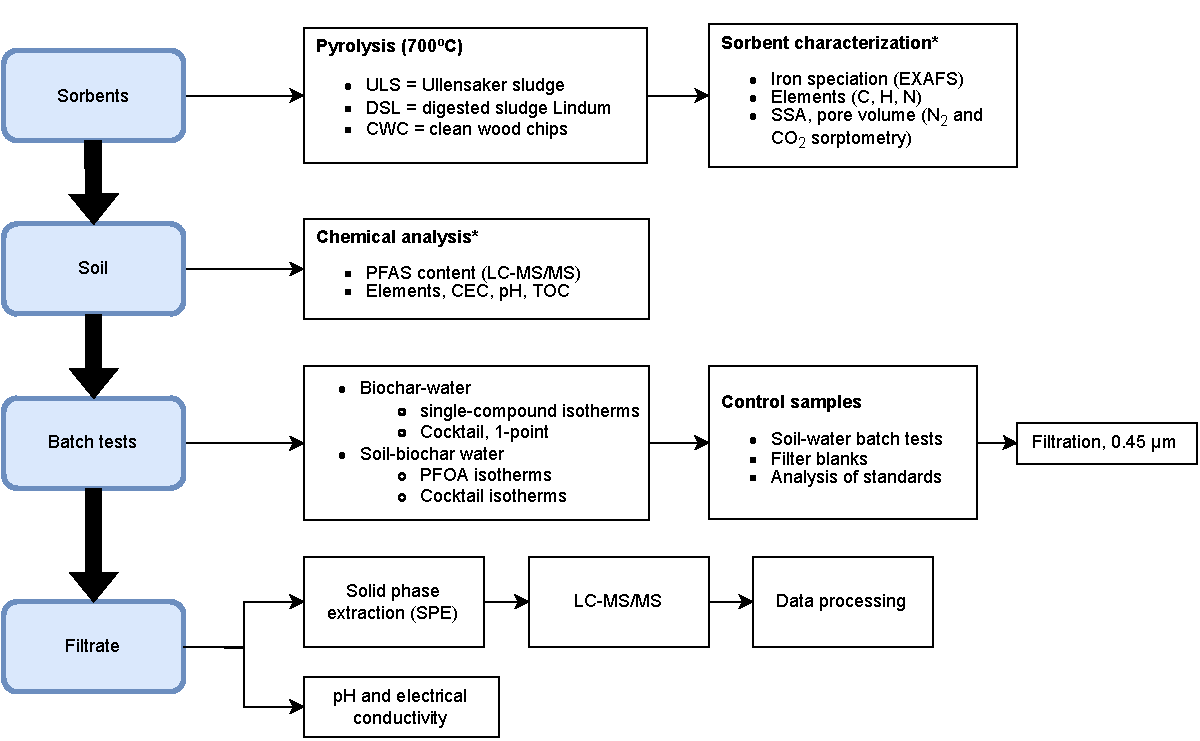
\includegraphics[width=\textwidth]{Diagrams/Methods-General_overview_methods.pdf}
    \caption{Overview of the methods conducted for this thesis. * = analyses conducted by commercial laboratories or that were delegated to project partners.}
    \label{fig:methodoverview}
\end{figure}

\section{Biochar sorbents}

\subsection{Feedstock}
Been banned with new guidelines and regulations but there is still much left in the unsaturated zone heavily contaminated with PFAS (what are the concentrations of the various PFASs?) NGI document? Firefighting training site at Gardermoen, Norway used these substances since 1989. Ullensaker sludge

Three feedstock types were selected as sorbents in the sorption experiments: Ullensaker Sludge (ULS), Digested Sludge Lindum (DSL) clean wood chips (CWC). ULS is raw sewage sludge from Ullensaker WWTP that has been dewatered. DSL is sludge from food waste and organic material that has been through anaerobic digestion (AD) to produce biogas, also referred to as digestate. Anaerobic digestion is performed at Lindum AS and produces methane (and other gases: 

\begin{equation}
\label{eq:AD}
    \ce{C_cH_hO_oN_nS_s + yH_2O -> xCH_4 + nNH_3 + xH_2S + (c-x)CO_2}
\end{equation}

which becomes commercial biogas fuel. The sewage sludge is dewatered, dried and pelletized before pyrolysis. CWC is made of clean, fresh softwood timber without additives that have been shredded, dried, and compressed into 8 mm pellets. The wood pellets are commercially available from Hallingdal trepellets (Kleivi næringspark, Ål).

\subsection{Pyrolysis}
CWC, ULS, and DSL biochars were produced by slow pyrolysis at 700 \textdegree C using ETIA technology by Biogreen\textsuperscript{\textcopyright} at Lindum AS (Drammen, Norway). \cref{tab:sorbents} summarizes the variables for pyrolysis of each biochar. The three biochars were produced as part of a larger study on the life cycle of waste based sorbents and was given as biochar samples to conduct the sorption experiments on for this thesis. The pyrolysis chamber is first electrically heated to stable PT. Feedstock pellets are added to a feeding container where a heated rotating screw (Spirajoule\textsuperscript{\textregistered}) transports the feedstock into and through the pyrolysis chamber at the programmed RT. The biochar is then transported to an external collection container where it is dispensed into sampling bags \cref{fig:biocharCollection}. \cref{fig:pellets} shows the pellets before and after pyrolysis. 

\begin{table}
\centering
\caption{Pyrolysis temperature (PT), residence time (RT) and feedstock for the biochars used in the sorption experiments.}
\label{tab:sorbents}
\begin{tabular}{llll}
\toprule
Biochar   & PT & RT & Feedstock \\
sorbent & (\textdegree C) & (min) \\
\midrule
CWC  & 700 & 20 & clean wood chips  \\
ULS & 700 & 40  & Ullensaker sludge\\
DSL & 700 & 20 & Digested sludge Lindum \\
\bottomrule
\end{tabular}
\end{table}

\begin{figure}
    \centering
    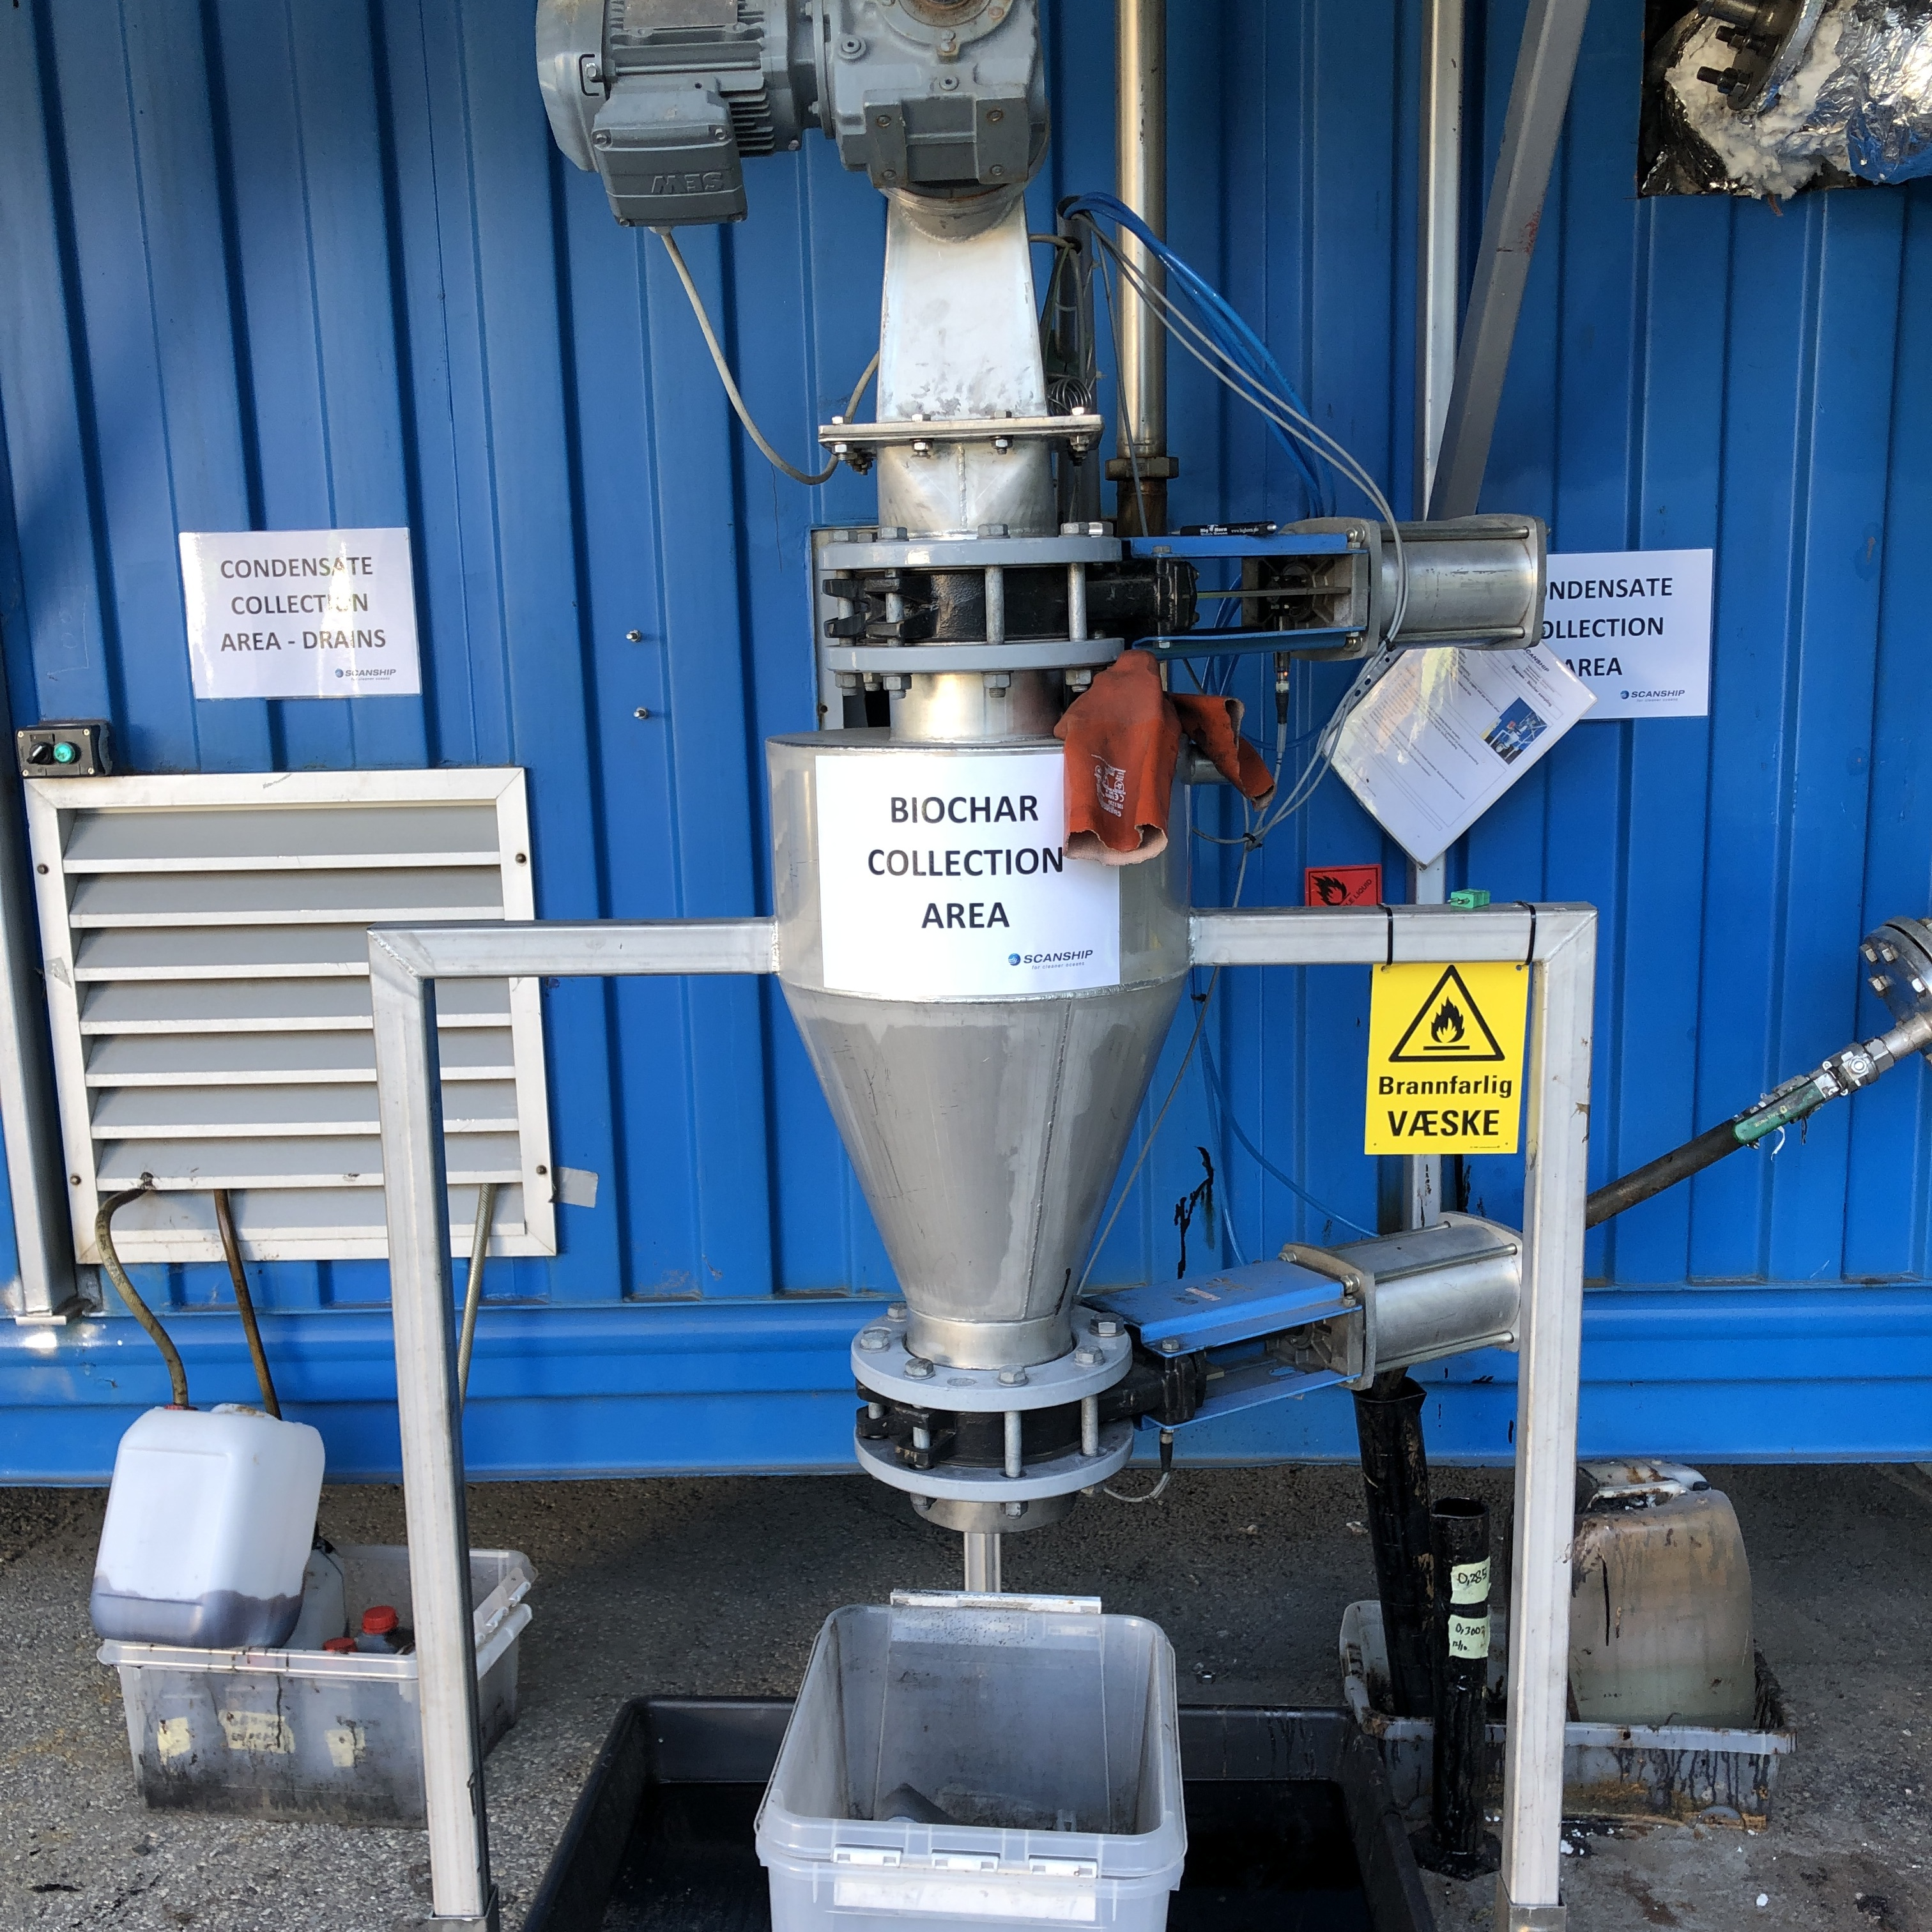
\includegraphics[width=0.6\linewidth,scale=0.6]{Bilder/Pyrolysis/BiocharCollection.jpg}
    \caption{Biochar collection area.}
    \label{fig:biocharCollection}
\end{figure}

\begin{figure}
    \centering
    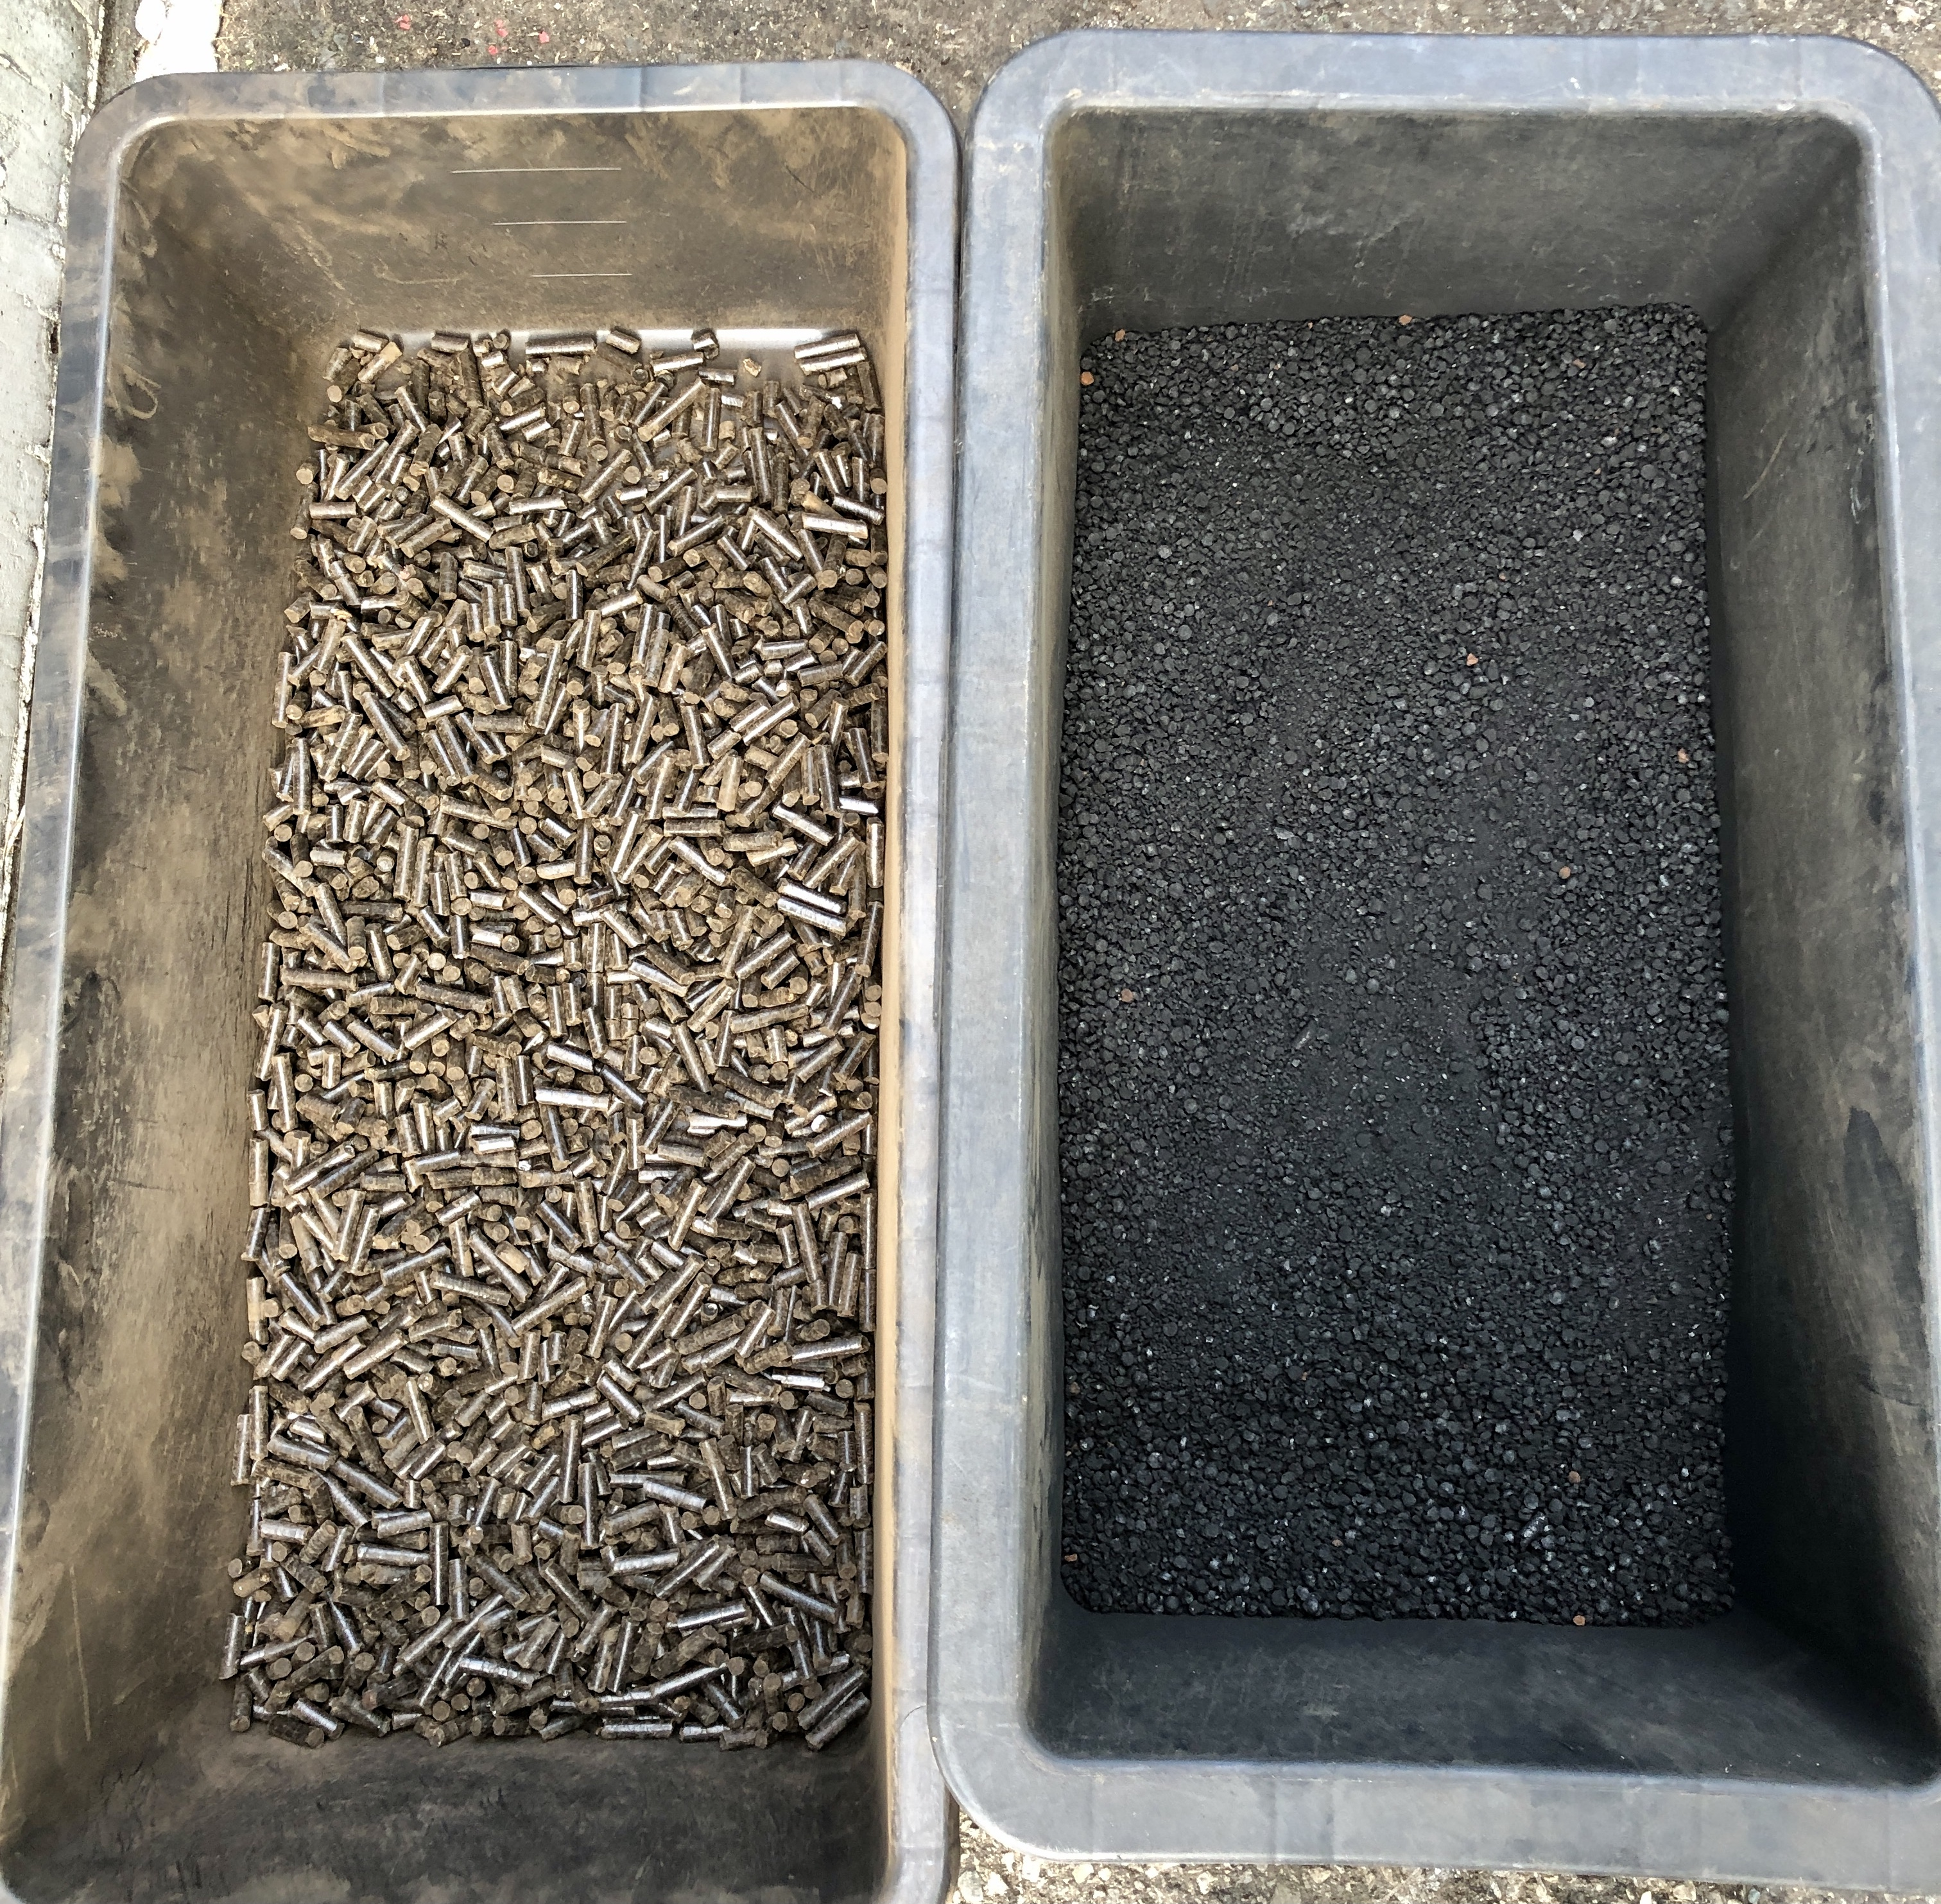
\includegraphics[width=0.6\linewidth,scale=0.6]{Bilder/Pyrolysis/Pellets.png}
    \caption{DSL feedstock pellets (left) and pyrolyzed pellets/biochar (right).}
    \label{fig:pellets}
\end{figure}

Syn-gas from pyrolysis is led through a condensing pipe that condenses into bio-oil at two points depending on boiling point. Syn-gas that does not condense at this point is led into a combustion chamber where a steady inflow of propane ensures a clean burning process of the remaining molecules.

\subsection{Biochar characterization}

\subsubsection{Surface area and pore volume}
Total specific surface area and pore volume were determined by $\mathrm{N_2}$ and $\mathrm{CO_2}$ gas sorptiometry by research partners at the Particle Engineering Research Center, University of Florida (Gainesville, USA) with a Quantachrome Autosorb 1 surface area analyzer according to the methods described by \cite{kwon2005}.  $\mathrm{N_2}$ sorptiometry was performed at the boiling point for liquid nitrogen (-195.8 \textdegree C). Due to slow diffusion at this low temperature, sorption of  $\mathrm{N_2}$ represents the largest pores of \textgreater 1.5 nm. $\mathrm{CO_2}$ sorptiometry was performed at 0 \textdegree C, and the higher temperature allows the gas to diffuse into smaller pores between 0.4-1.5 nm. $\mathrm{N_2}$ surface area was interpreted using Brunauer, Emmett and Teller (BET) theory, pore size and volume using Barret-Joyner-Halenda (BJH) theory, and $\mathrm{CO_2}$ surface area and pore volume were evaluated using density functional theory (DFT) theory . 

\subsubsection{Element analysis}
Elemental composition (total C, H and N) was performed by $\mathrm{NO_3}$ digestion and quantified with a Leco CHN-1000 from Leco Corporations (Sollentuna, Sweden), according to DIN 51732 by project partner.  

\subsubsection{Iron speciation}
Iron and copper speciation of DSL and ULS were analyzed by Fe K-edge X-ray absorption fine structures (EXAFS) at the synchrotron SOLEIL (Gif-sur-Yvette, France) (beamline SAMBA) by a project colleague at NGI. To prepare the biochars for analysis, each sample ($\sim$50 mg) was crushed with a mortar to a fine powder (250 \textmu m). The samples were mixed with boron nitride (BN, 300 mg) to a homogeneous powder and pelletized. BN matrix is used for sample dilution because it absorbs very little of the photon beam at the Fe K-edge. The biochar pellet was then analyzed by X-ray absorption spectroscopy.  

The overall principle of EXAFS is to determine structural composition of a sample by examining its X-ray absorption spectrum, which plots absorbance, $\mu x$, as a function of photon energy, $eV$ \citep{vlaica2004exafs}. The sample is submitted to an X-ray beam where a spectrophotometer measures the beam intensity going through the sample. The difference of intensity between before and after the sample is translated into an absorption coefficient, following Beer-Lambert's Law: 

\begin{equation}\label{eq:absorbance}
    \mu x = log \frac{I}{I_0}
\end{equation}

where $\mu x$ is a dimensionless absorbance coefficient ($AU$), $I$ is the transmitted light intensity and $I_0$ is the incident light intensity. The energy of the photon beam is determined by the angle of a crystal monochromator. The angle of the crystal monochromator is tuned so that the sample is submitted to a range of photon energies in which the absorption edges of the target element lie within \citep{vlaica2004exafs}. An adsorption K-edge occurs when the transmitted photon energy equals the energy required to excite a core electron, which is observed as a vertical jump (K) in $\mu x$ on the spectrum \citep{vlaica2004exafs}. The neighboring elements are interfering with the photon wave, which translates into oscillations on the absorption spectrum following the absorption edge. Each element has a different retrodiffusion coefficient, therefore the frequency and amplitude of oscillations in the absorption spectrum are (partially) determined by the type and number of neighboring atoms. The absorption edge energy and the oscillations thus contain information on the valency of the element and number and type of neighboring atoms, i.e., the element speciation. Fe(II) species will have K at a lower energy than Fe(III) species because a higher photon energy is required to excite an electron from the more electronegative Fe(III). In addition, the oscillations will differ depending on the Fe mineral. By interpreting the X-ray absorption spectrum, the different iron species present in the sample can be derived.

%%%%%%%%%%%%%%%%%%%%%%%%%%%%%%%%%%%%%%%%%%%%%%%%%%%%%%%%%%%%%%%%%%%%%%%%%%%%%%%%%%%%%%%%%%%%%%%%%%%%%%%%%%%%%%%

\section{Sorption experiments}
Effectiveness of PFCA removal by waste biochar was evaluated by batch shaking tests. The following section describes how the batch tests were prepared.

\subsection{Experiment preparations}
\subsubsection{Target compounds}\label{sec:PFCAanalytic}
6 perfluorinated carboxylic acids (PFCAs), perfluoropentanoic acid (PFPeA), perfluorohexanoic acid (PFHxA), perfluoroheptanoic acid (PFHpA), perfluorooctanoic acid (PFOA), perfluorononaoic acid (PFNA), perfluorodecanoic acid (PFDA), with perfluorinated carbon (PFC) units 4-9 respectively were selected as target compounds (TCs) for the batch test experiments in this thesis. See \cref{tab:PFCAs} for a list of all native PFCAs including their respective CAS numbers included in this thesis. 10 mL stock solutions were prepared for each TC by weighing the pure PFCA salts/liquid (\cref{tab:PFCAs}) on an analytical scale and dissolving them in methanol in volumetric flasks. Two spiking standards at a high (STD1) and low (STD2) concentration were prepared from the stock solution to be used for spiking the batch tests at various concentrations (\cref{apptab:standards}). The working standards were analyzed with LC-MS/MS of a 2-time diluted standard at an optimum concentration for the instrument calibration curve (10-20 \textmu g L\textsuperscript{-1}, \cref{appSec:IsothermSetup}) and all further calculations of spike dilutions were corrected with the measured standard concentrations.

\begin{table}
\centering
\caption{PFAS compounds investigated in this study. PFCs correspond to the number of perfluorinated carbon units in the chain. Note: PFCAs appear in dissociated form at environmentally relevant pH's due to low $pK_a$'s.}
\adjustbox{max width=\textwidth}{
\label{tab:PFCAs}
\begin{tabular}{@{}lcccclc@{}}
\toprule
\multicolumn{1}{c}{Chemical} & Acronym & Short & CAS number & Molecular structure & Stock form & Purity \\ \midrule
& & & & & &\\
\smash{\raisebox{4ex}{Perfluoropentanoic acid}}  & \smash{\raisebox{4ex}{PFPeA}} & \smash{\raisebox{4ex}{C5}} & \smash{\raisebox{4ex}{2706-90-3}} & \chemfig[atom style={scale=0.4}]{O=[:90](-[:30,,,1]OH)-[:150](-[:112.5]F)(-[:67.5]F)-[:210](-[:292.5]F)(-[:247.5]F)-[:150](-[:112.5]F)(-[:67.5]F)-[:210](-[:270]F)(-[:150]F)-[:210]F} & \smash{\raisebox{4ex}{liquid}} & \smash{\raisebox{4ex}{\textgreater 97 \%}} \\
& & & & & &\\
\smash{\raisebox{4ex}{Perfluorohexanoic acid}} & \smash{\raisebox{4ex}{PFHxA}}  & \smash{\raisebox{4ex}{C6}} & \smash{\raisebox{4ex}{307-24-4}} & \chemfig[atom style={scale=0.4}]{O=[:90](-[:30,,,1]OH)-[:150](-[:112.5]F)(-[:67.5]F)-[:210](-[:292.5]F)(-[:247.5]F)-[:150](-[:112.5]F)(-[:67.5]F)-[:210](-[:292.5]F)(-[:247.5]F)-[:150](-[:210]F)(-[:150]F)-[:90]F} & \smash{\raisebox{4ex}{liquid}} & \smash{\raisebox{4ex}{\textgreater 97 \%}} \\
& & & & & &\\
\smash{\raisebox{4ex}{Perfluoroheptanoic acid}} & \smash{\raisebox{4ex}{PFHpA}} & \smash{\raisebox{4ex}{C7}} & \smash{\raisebox{4ex}{375-85-9}} & \chemfig[atom style={scale=0.4}]{O=[:90](-[:30,,,1]OH)-[:150](-[:67.5]F)(-[:112.5]F)-[:210](-[:247.5]F)(-[:292.5]F)-[:150](-[:67.5]F)(-[:112.5]F)-[:210](-[:247.5]F)(-[:292.5]F)-[:150](-[:67.5]F)(-[:112.5]F)-[:210](-[:150]F)(-[:210]F)-[:270]F} & \smash{\raisebox{4ex}{crystalline}} & \smash{\raisebox{4ex}{\textgreater 99 \%}} \\
& & & & & &\\
\smash{\raisebox{4ex}{Perfluorooctanoic acid}} & \smash{\raisebox{4ex}{PFOA}}  & \smash{\raisebox{4ex}{C8}} & \smash{\raisebox{4ex}{335-76-2}}  & \chemfig[atom style={scale=0.4}]{O=[:90](-[:30,,,1]OH)-[:150](-[:67.5]F)(-[:112.5]F)-[:210](-[:247.5]F)(-[:292.5]F)-[:150](-[:67.5]F)(-[:112.5]F)-[:210](-[:247.5]F)(-[:292.5]F)-[:150](-[:67.5]F)(-[:112.5]F)-[:210](-[:247.5]F)(-[:292.5]F)-[:150](-[:90]F)(-[:150]F)-[:210]F} & \smash{\raisebox{4ex}{powder}} & \smash{\raisebox{4ex}{\textgreater 95 \%}} \\
& & & & & &\\
\smash{\raisebox{4ex}{Perfluorononaoic acid}}  & \smash{\raisebox{4ex}{PFNA}} & \smash{\raisebox{4ex}{C9}} & \smash{\raisebox{4ex}{375-95-1}} & \chemfig[atom style={scale=0.4}]{O=[:90](-[:30,,,1]OH)-[:150](-[:112.5]F)(-[:67.5]F)-[:210](-[:292.5]F)(-[:247.5]F)-[:150](-[:112.5]F)(-[:67.5]F)-[:210](-[:292.5])(-[:247.5]F)-[:150](-[:112.5]F)(-[:67.5]F)-[:210](-[:292.5]F)(-[:247.5]F)-[:150](-[:112.5]F)(-[:67.5]F)-[:210](-[:270]F)(-[:210]F)-[:150]F} & \smash{\raisebox{4ex}{crystalline}} & \smash{\raisebox{4ex}{\textgreater 97 \%}} \\
& & & & & &\\
\smash{\raisebox{4ex}{Perfluorodecanoic acid}}  & \smash{\raisebox{4ex}{PFDA}}  & \smash{\raisebox{4ex}{C10}} & \smash{\raisebox{4ex}{335-67-1}} & \chemfig[atom style={scale=0.4}]{O=[:90](-[:30,,,1]OH)-[:150](-[:112.5]F)(-[:67.5]F)-[:210](-[:292.5]F)(-[:247.5]F)-[:150](-[:112.5]F)(-[:67.5]F)-[:210](-[:292.5]F)(-[:247.5]F)-[:150](-[:112.5]F)(-[:67.5]F)-[:210](-[:292.5]F)(-[:247.5]F)-[:150](-[:112.5]F)(-[:67.5]F)-[:210](-[:292.5]F)(-[:247.5]F)-[:150](-[:210]F)(-[:150]F)-[:90]F} & \smash{\raisebox{4ex}{flakes}} & \smash{\raisebox{4ex}{\textgreater 98\%}} \\
& & & & & &\\ \bottomrule
\end{tabular}}
\end{table}

\subsubsection{Spike concentrations}
Sorption of PFAS to biochar follows the Freundlich sorption model, which means that sorption increases linearly until it is attenuated at higher concentrations \cref{eq:Freundlich}. Details on sorption models is provided in \cref{sec:data_analysis} The goal when designing the sorption isotherm experiments was to represent sorption across both the linear and non-linear region. To achieve detectable concentrations across this range, determination of appropriate spike concentrations was based on several factors: 1) Biochar-water partition coefficients ($K_{BC}$) for the TCs obtained from literature \cite{Xiao2017} \cref{tab:Kbc}, 2) biochar dose, 3), the LOQ of the analytical method, and 4) available pipetting volume range. The relationship between $K_{BC}~\mathrm{(L~g^{-1})}$, the sorbed concentration, $C_s~\mathrm{(\mu g~g^{-1})}$, and the freely dissolved aqueous concentration, $C_w~\mathrm{(\mu g~L^{-1})}$, expressed as:

\begin{align}
    \label{eq:Kbc1}
    K_{d} = \frac{C_s}{C_w}
\end{align}

was used to estimate the expected $C_w$. By rearranging \cref{eq:Kbc1},  $C_w$ is expressed as a function of the mass TA spiked and the estimated $K_d$:

\begin{align}
    \label{eq:Cw2}
    C_w=\frac{\frac{m_{PFAS}}{\left (\frac{m_{BC}\times K_{BC}}{V_w}\right)+1}}{V_w}
\end{align}

Where $m_{TA}$ is the mass PFAS spiked, $m_{BC}$ is the biochar dose, and $V_w$ is the volume of the sample matrix. Using \cref{eq:Cw2}, the lowest spike concentration for each isotherm was taken to be two times the method LOQ for the LC-MS/MS instrument at NTNU, Trondheim (\cref{apptab:LOQ}). The remaining points were spread evenly over a $10^4$ concentration interval. 

\begin{table}
\centering
\caption{Biochar-water distribution coefficients ($K_{BC}$) for PFCAs derived from \cite{XiaoSI2017}.} 
\label{tab:Kbc}
\begin{threeparttable}
    \begin{tabular}{@{}lcc@{}}
    \toprule
    \multicolumn{1}{l}{\begin{tabular}[l]{@{}l@{}}Compound\end{tabular}} &  \multicolumn{1}{c}{\begin{tabular}[c]{@{}c@{}}log $\mathrm{K_{BC}}$\\ \citep{XiaoSI2017}\end{tabular}} & \multicolumn{1}{c}{\begin{tabular}[c]{@{}c@{}}est. log $\mathrm{K_{BC}}$ \end{tabular}} \\ \midrule
    PFPeA & 4.16 & 4.16 \\
    PFHxA & 4.15 & 4.15 \\
    PFHpA & 4.49 & 4.49 \\
    PFOA & 4.76 & 4.76 \\
    PFNA & *4.89 & 4.89 \\
    PFDA & *5.09 & 5.09 \\ \bottomrule             
    \end{tabular}
\begin{tablenotes}
\item * not included in \citep{XiaoSI2017}, so the values are extrapolated from the shorter chain lengths.
\end{tablenotes}
\end{threeparttable}
\end{table}

Two preliminary batch tests were prepared to check how well the $K_d$ values selected from the literature corresponded to those for ULS and CWC. Further details about this analysis are provided in \cref{appSec:IsothermSetup}.

\subsubsection{Biochar}
A sub sample (100 g) was taken by random grab sampling from the bulk volume of the biochar produced during pyrolysis. The biochars were crushed using a ball mill (Retsch ISO 9001) with five balls at 50 rpm for 5 minutes and sieved into fine-powdered biochar (D \textless 1 mm) and transferred to LDPE zipper bags for storage (4 \textdegree C). 

\subsubsection{Soil}
The soil used for the sorption tests was an unaged sandy soil obtained from a remote field area 17 km from Uppsala, Sweden (59.733 N, 17.667 E). The carbon and nitrogen content in the soils was determined through dry combustion according to ISO10694 (1995) and ISO 13878 (1998), respectively using an elemental analyzer for macrosamples (TruMac ® CN, Leco corp, S:t Joseph, MI, USA).... pH according to...  The soil was characterized for total element concentrations, exchangeable ions, TOC and pH by... the methods... by research partner

The soil was dried at 100 \textdegree C for 24 h and crushed and sieved to \textless 2 mm.  The soil was screened for PFAS using a methanol extraction, solid phase extraction and quantification by liquid chromatography coupled with tandem mass spectrometry at NTNU (Trondheim, Norway) by a project partner (details for the SPE and LC-MS/MS procedures will be given in \cref{methods:instrAnalysis}), performed in triplicate.

\begin{figure}
    \centering
    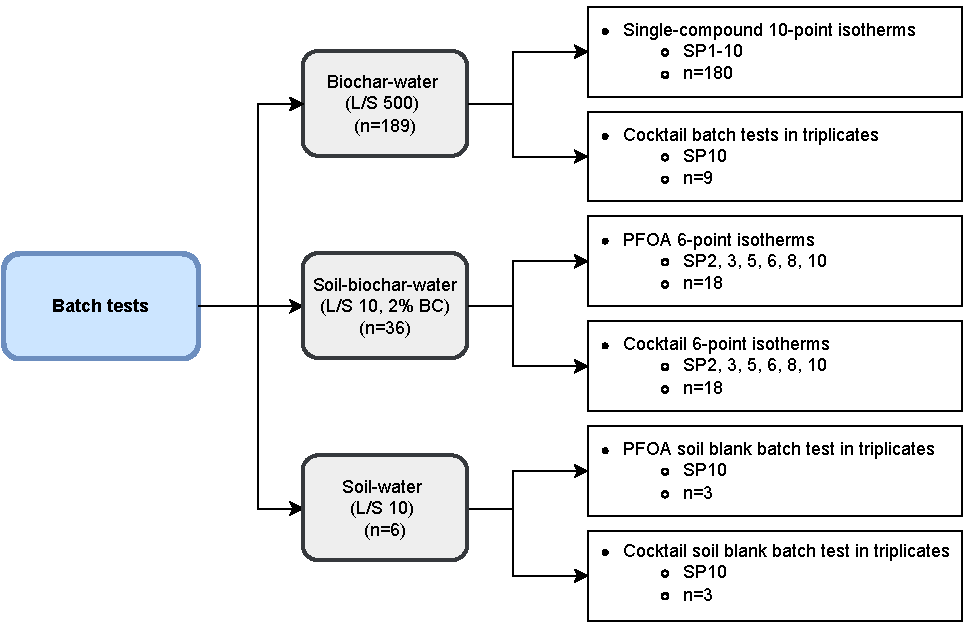
\includegraphics{Diagrams/Methods-Page-9.pdf}
    \caption{Overview of batch test samples for this thesis for the three biochars (ULS, DSL, CWC) and six TCs.}
    \label{fig:batchtests_flowchart}
\end{figure}

\begin{figure}
    \centering
    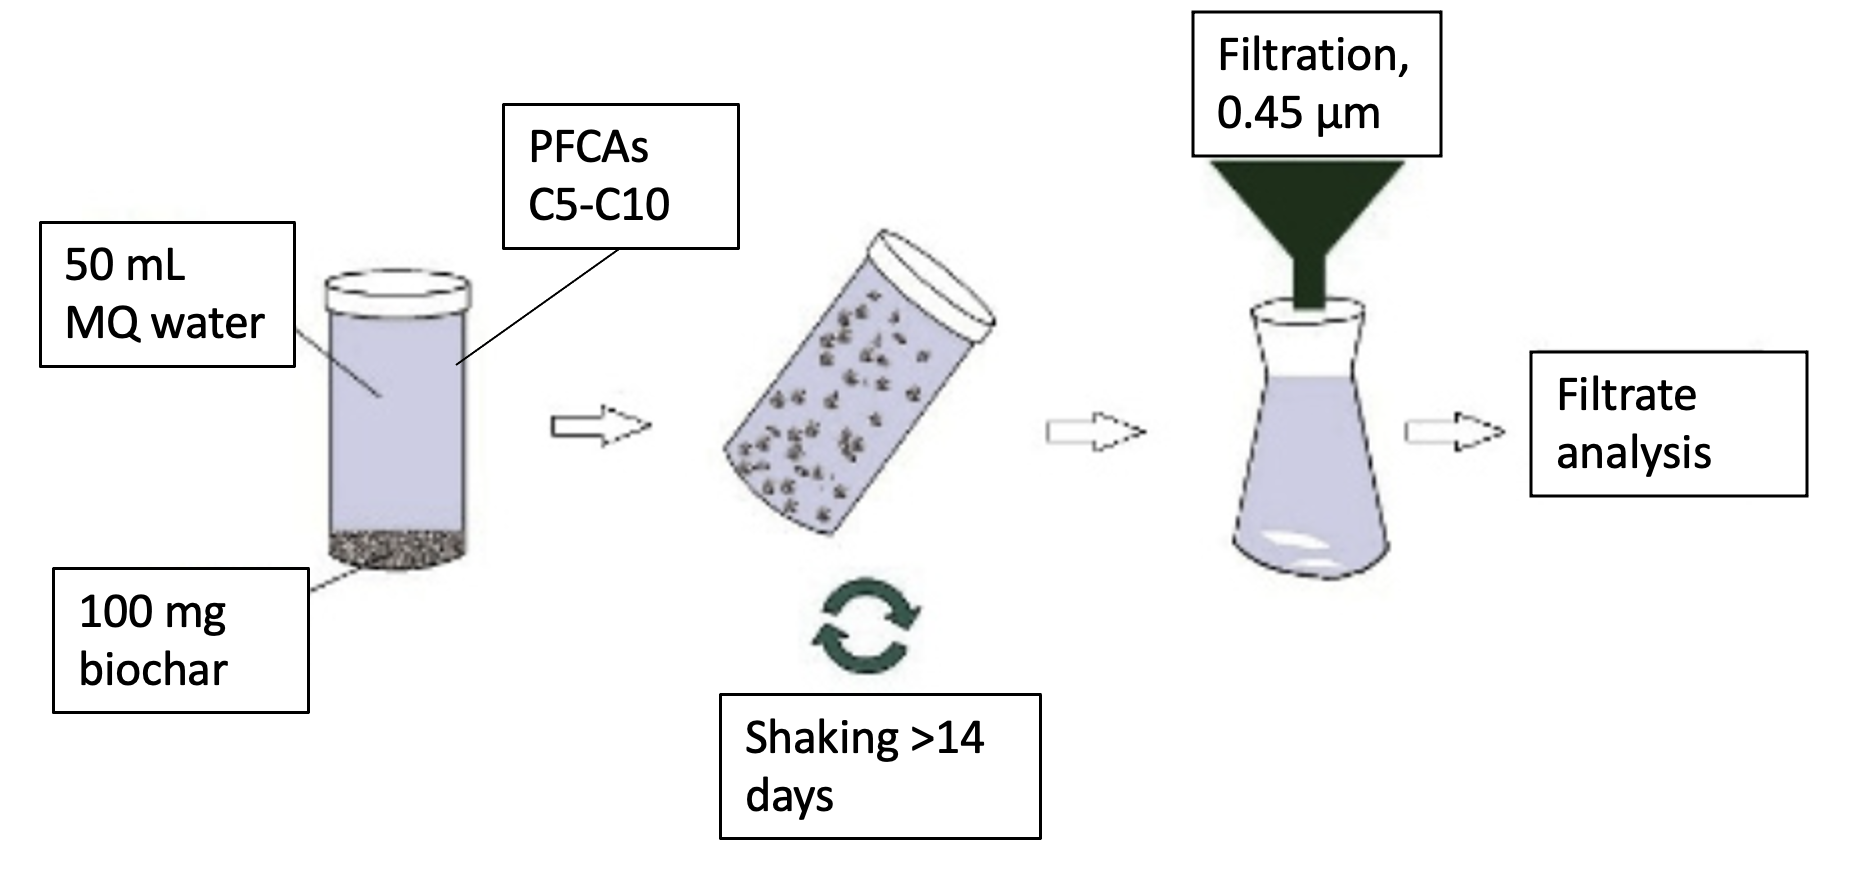
\includegraphics[width=\textwidth]{Diagrams/Batch_test.png}
    \caption{Batch test experimental procedure.}
    \label{fig:batchtest_setup}
\end{figure}

\begin{table}
    \caption{Spike concentrations (SC) in \textmu g L\textsuperscript{-1} used for the batch tests. MIX = cocktail spike concentration for biochar-water batch tests in triplicates, MIX-S = cocktail spike concentration for biochar-soil-water and soil-water batch tests.}
    \label{tab:spikeConcentrations}
    \adjustbox{max width=\textwidth}{%
    \begin{tabular}{lrrrrrrrrrrrr}
    \toprule
    \textbf{Compound} & \textbf{SC1} & \textbf{SC2} & \textbf{SC3} & \textbf{SC4} & \textbf{SC5} & \textbf{SC6} & \textbf{SC7} & \textbf{SC8} & \textbf{SC9} & \textbf{SC10} & \textbf{SC10-MIX} & \textbf{SC10-MIX-S} \\ \midrule
    PFPeA & 0.019 & 21 & 43 & 64 & 86 & 107 & 128 & 150 & 171 & 191 & 191 & 283\\
    PFHxA & 0.033 & 37 & 73 & 110 & 146 & 184 & 220 & 256 & 292 & 330 & 330 & 836 \\
    PFHpA & 0.012 & 11 & 25 & 38 & 52 & 65 & 79 & 92 & 106 & 117 & 117 & 153\\
    PFOA & 0.195 & 216 & 435 & 651 & 871 & 1 087 & 1 302 & 1 522 & 1 742 & 1 953 & 1 953 & 1 974\\
    PFNA & 0.141 & 156 & 313 & 471 & 625 & 784 & 942 & 1 097 & 1 255 & 1 409 & 1 409 & 2 310\\
    PFDA & 0.383 & 425 & 850 & 1 275 & 1 700 & 2 126 & 2 551 & 2 976 & 3 401 & 3 830 & 3 830 & 5 288\\ \bottomrule
    \end{tabular}}
\end{table}

\subsection{Batch tests}
An overview of the experimental setup for the batch test is given in \cref{fig:batchtests_flowchart} and an illustration of the overall batch test experiment procedure is in \cref{fig:batchtest_setup}. Details for the preparations of each batch test category are given in the subsections below. The batch tests were prepared with a liquid to solid mass ratio (L/S) of 500 for biochar and L/S of 10 for soil amended with 2\% biochar in accordance with CEN EN 12457. All PP tubes were rinsed three times with 50\% MeOH and dried prior to sample preparation to extract any potential PFAS contamination. The dry matter was added to pre-cleaned 50 mL PP centrifuge tubes and spiked with either individual PFCAs or a cocktail of all six TCs at the concentrations specified in \cref{tab:spikeConcentrations} to a final liquid volume of 50 mL. The standard concentrations were analytically verified to ensure accuracy of the data analysis (see \cref{appSec:IsothermSetup} for expected vs. analytical concentrations). The samples were assured to contain \textless 10\% MeOH, which is the upper limit for which methanol does not influence sorption (reference). The batch tests were shaken end-over-end (9 rpm) and/or agitated on a shaking table (160 rpm) in room temperature (20\textdegree C) for at least 14 days to reach equilibrium \citep{higgins2006sorption} before filtration through a 0.45 \textmu m Minisart\textsuperscript{\textregistered} regenerated cellulose syringe filter into PP tubes based on the methods described in \cite{Sorengard2019}. Loss of biochar to the walls of the syringe was quantified to maintain a full mass balance when analyzing the partitioning of the TCs between the solid and liquid phase and is in \cref{appSec:misclab}. Therefore, a 100\% mass balance was assumed when calculating partitioning between sorbent and water by subtracting the initial spike concentration from the measured concentration in the filtrates. by also correcting for loss to laboratory ware (reference). 

\subsubsection{Biochar-water batch tests}
100\textpm 4 mg biochar was weighed for the biochar-water batch tests. on an analytical scale and placed into pre-cleaned (50\% methanol) 50 mL PP tubes. The tubes were filled half up of Milli-Q water. In each tube, stock PFCA was pipetted using micro- (5-50 {\textmu}l and 200-1000 {\textmu}L) and milli pipettes (2-10 mL) into the char-water solution to make 10 dilutions for each of the 6 PFCAs in even intervals within the concentration points in \cref{tab:spikeConcentrations}. Some tubes were added Milli-Q water up to the 50 mL mark and some were weighed in order to control for the water amount being within \textpm 0.02 mL. The same ten concentrations were used to spike CWC, ULS and DSL batch tests. A cocktail batch test was prepared for the three biochars using the same relative amounts of each TC as the single-spike samples at SC10 (SC10-MIX), which was spiked directly into the sample tubes. The same dose biochar was used as for the other sorption isotherms. The cumulative CMC (critical micelle concentration) for the six PFCAs at SC10 was assured not to be an issue for the concentration range considered \citep{bhhatarai2011,ding2013physicochemical}.

\subsubsection{Soil-biochar-water batch tests}\label{sec:S-BC}
5\textpm 0.005 g soil and 0.1\textpm 0.0004 g biochar were weighed for each soil-BC-water batch test. A cocktail standard was prepared before spiking the samples using the same proportions at SC10 as for the biochar-water batch test. The difference between the two methods used to spike cocktail samples is a potential source of error for later comparison of sorption attenuation. 
The batch tests were prepared as 6-point isotherms within a 10\textsuperscript{4} concentration range with a L/S ratio of 10 in PP tubes, in accordance with CEN EN 12457 with modifications described in \citep{Hale2017fire,Kupryianchyk2016a}. L/S 10  is common in leaching tests for waste materials and soil according to the waste and shaken in an end-over-end shaker for \textgreater 14 days. 
centrifuged to remove as many particles from suspension as possible. Still, filtration required frequent filter change due to clogging (up to three times per sample).

\subsection{pH and electrical conductivity}
pH and conductivity was measured in a solution (1:5) of biochar and water, with pre-stirring (15 min) and letting the particles settle (\textgreater 24 hrs) before measurement (n=3). This is according to the standard method for measuring pH in soil. It is common to add CaCl\textsubscript{2} if the soil has a low ionic strength, but this was considered unnecessary in the presence of biochar as it contains a high amount of soluble ions. 

\subsection{Control samples}
To control for potential underestimation of $C_w$, filter blanks were prepared for each PFCA in triplicates at an optimum concentration range for the instrument (see \cref{sec:PFCAanalytic}) to correct for PFCA loss to the filter paper. 

%%%%%%%%%%%%%%%%%%%%%%%%%%%%%%%%%%%%%%%%%%%%%%%%%%%%%%%%%%%%%%%%%%%%%%%%%%%%%%%%%%%%%%%%%%%%%%%%%%%%%%%%%%%%%%%%%%%%%%%%%%%%

\section{Instrumental analysis} \label{methods:instrAnalysis}
PFAS quantitation in the filtrates were determined by liquid chromatography--tandem mass spectrometry (LC-MS/MS). Reversed phase solid phase extraction (SPE) was used as sample preparation method. The analyses were conducted at the Institute of Chemistry at NTNU (Trondheim, Norway).

% missing reconstitution step, update diagram
\begin{figure}
    \centering
    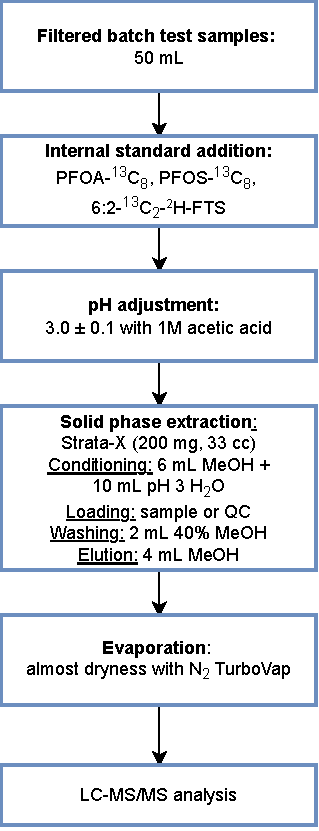
\includegraphics{Diagrams/Methods-Analytical_method.pdf}
    \caption{Schematic diagram of the analytical method applied for the determination of TCs in the batch test filtrates adapted from \cite{arvaniti2012diagram}.}
    \label{fig:analyticalMethod}
\end{figure}

\subsection{SPE}
SPE is a sample preparation method used to concentrate a large-volume sample to an extract that can be submitted for analyte quantitation by LC-MS/MS. The sample is passed through a cartridge with a porous sorbent polymer that strongly retains polar compounds (\textpi-\textpi bonding, hydrogen bonding and hydrophobic interaction). The sorbed analytes are then eluted with an appropriate solvent, evaporated, and finally reconstituted to the desired extract volume. All samples are spiked with a mix of internal standards (ISs) to compensate for variations in extraction percentages and instrumental response by the MS/MS detector \citep{arvaniti2014}. To minimize risk of contamination during laboratory work, working benches were cleaned with acetone and covered with aluminum foil. Sterilized PP tubes were used during all steps of the protocol.

Strata-X\textsuperscript{\textregistered} 200 mg/6mL cartridges supplied by Phenomenex were used for SPE of the TCs in the filtered water samples. The sorbent polymer was a surface modified styrene divinylbenzene (\cref{fig:StatPhase}) with 33 \textmu m average particle diameter and surface area of 800 m\textsuperscript{2} g\textsuperscript{-1}. The internal standards used were \textsuperscript{13}C\textsubscript{8}-perfluorooctanoic acid  (\textsuperscript{13}C\textsubscript{8}-PFOA), \textsuperscript{13}C\textsubscript{8}-potassium perfluorooctanesulfonate (\textsuperscript{13}C\textsubscript{8}-PFOS-K), and 6:2-\textsuperscript{13}C\textsubscript{2}-\textsuperscript{1}H,\textsuperscript{2}H-perfluorooctane sulfonate  (6:2 \textsuperscript{13}C\textsubscript{2}-FTS) where a working standard of the three isotopic PFAS was prepared in methanol at 1 ppm from 50 ppm analytical standard supplied by Sigma Aldrich.

The samples were adjusted to pH $\sim$3 with 800 \textmu L 1 M acetic acid. However, the samples containing soil needed addition of at least double the amount to reach the same pH. pH was tested for five randomly selected samples for each batch of 20 was with pH strips. All samples were then spiked with IS. SC1 and SC2 samples were spiked with 10 \textmu L IS and SC3-SC10 samples were spiked with 20 \textmu L IS--the difference in amount of IS for the two low-spike samples being due to a more concentrated extract needed for these samples to avoid signals below instrumental LOQ. Therefore, SC1 and SC2 samples were made to 0.5 mL extracts instead of 1 mL as for the rest. The samples were vortexed prior to SPE.

The cartridges were placed in individual slots with LC liners on a TLC chamber and conditioned with 6 mL MeOH and 10 mL pH 3 milli-Q water (acidified by 100\% acetic acid). MeOH was used for wetting to allow the mobile phase into the pores of the sorbent polymer in order to ensure maximum chromatographic retention. Low-pH water was used to protonate loan electrons on the polymer surface so that hydrophobic interaction with the analytes were maximized. The samples were loaded using glass pipettes and allowed to pass through the cartridges with gravity. The flow rate was adjusted by modifying the opening of the LC liners so that the sample exited the cartridge as individual droplets. 

After loading the samples, the cartridges were washed with 2 mL MeOH:MQ (40:60, \% v/v) in order to remove any matrix interferences. The cartridges were then dried with a vacuum pump at 20 mmHg until the sorbent mass was visible as dry powder. The analytes were eluted with 4 mL MeOH into 15 mL PP centrifuge tubes, and concentrated to almost dryness ($\le$0.5 mL) using TurboVap\textsuperscript{\textregistered} at 40 \textdegree C and nitrogen gas (N\textsubscript{2}) at 5 psi. The samples were reconstituted to 1 mL (0.5 mL for SCs 1 and 2) with MeOH and milli Q to a final solvent ratio of 50:50 \% v/v. The extracts were transferred to LC vials using glass pipettes and stored at -19 \textdegree C until analysis.

\begin{figure}
    \centering
    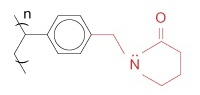
\includegraphics{Bilder/SPE_LCMS/mg_spe_strata-x.jpg}
    \caption{Sorbent polymer used for SPE, surface-modified styrene divinylbenzene.}
    \label{fig:StatPhase}
\end{figure}

\subsection{LC-MS/MS}
Liquid chromatography separates compounds in a mixture based on polarity by using a stationary phase that retards hydrophobic compounds while allowing more polar compounds to pass through faster along with the polar mobile phase. The compounds are then ionized by a strong voltage into fragment ions that are detected by a mass spectrometer that determines the mass of the transitions. Quantification of PFAS was determined by UPLC-MS/MS with an Acquity UPLC I-Class system connected to a Xevo TQ-S triple quadrupole mass spectrometer equipped with an ESI Z spray, both supplied by Waters (Milford, MA, USA). A Kinetex C18 column (30 x 2.1 mm, 1.3 \textmu m) serially connected to a Phenomenex C18 (2 x 2.1 mm i.d.) security guard (Torrance, CA, USA) was used for chromatographic separation. Mobile phases were A: 2 mM ammonium acetate in Milli-Q water (water phase) and B: pure MeOH (organic phase) that were supplied at a constant flow rate of 250 \textmu L min\textsuperscript{-1} to the LC column maintained at a temperature of 30 \textdegree C. The sample injection volume was 4 \textmu L. The run time for each sample was 6 minutes with an initial and final mobile phase gradient of 20:80 (A:B). Analytes were ionized by negative electrospray ionization (ESI-) and nitrogen was used as drying gas at the ionization source. Two ion transitions were monitored for each PFCA (\cref{tab:transitions}) within 60 s of the expected retention time for the compound. Peak integration was performed automatically by MassLynx software obtaining 12 points per peak and an average baseline peak width of 5 s. Data from UPLC-MS/MS was processed in MassLynx version 4.1 and quantification processing was performed with TargetLynx. Each peak was manually reviewed to remove peaks that were likely background noise as well as corrections for inconsistencies in peak base width. Complete instrument programming and parameters are summarized in \cref{appSec:LCMS}.

\begin{table}[tbh]
\centering
\caption{Ion transitions for the target analytes and internal standards in this study.}
\adjustbox{max width=\textwidth}{%
\begin{threeparttable}
\label{tab:transitions}
\begin{tabular}{ccccccl} \toprule
Compound &  Structure & Formula & M & Parent & Cone (V) & Transitions (CE)  \\ \midrule
& & & & & & \\
\multirow{2}{*}{PFPeA} &  \multirow{2}{*}{\chemfig[atom style={scale=0.5}]{O=[:90](-[:30,,,1]OH)-[:150](-[:112.5]F)(-[:67.5]F)-[:210](-[:292.5]F)(-[:247.5]F)-[:150](-[:112.5]F)(-[:67.5]F)-[:210](-[:270]F)(-[:150]F)-[:210]F}} & \multirow{2}{*}{$\mathrm{C_5HF_9O_2}$} & \multirow{2}{*}{264.05} & \multirow{2}{*}{262.97} & \multirow{2}{*}{20} & \multirow{2}{*}{262.97 $\rightarrow$ 219 (8)} \\
& & & & & & \\
& & & & & & \\
 &  &  &  &  &  &    \\
\multirow{2}{*}{PFHxA} &  \multirow{2}{*}{\chemfig[atom style={scale=0.5}]{O=[:90](-[:30,,,1]OH)-[:150](-[:112.5]F)(-[:67.5]F)-[:210](-[:292.5]F)(-[:247.5]F)-[:150](-[:112.5]F)(-[:67.5]F)-[:210](-[:292.5]F)(-[:247.5]F)-[:150](-[:210]F)(-[:150]F)-[:90]F}} & \multirow{2}{*}{$\mathrm{C_6HF_{11}O_2}$} & \multirow{2}{*}{314.05} & \multirow{2}{*}{312.97} & \multirow{2}{*}{10} & 312.97 $\rightarrow$ 118.95 (18) \\
 &  &  &  &  &  &   312.97 $\rightarrow$ 269 (8) \\
 & & & & & & \\
 & & & & & & \\
\multirow{2}{*}{PFHpA} &  \multirow{2}{*}{\chemfig[atom style={scale=0.5}]{O=[:90](-[:30,,,1]OH)-[:150](-[:67.5]F)(-[:112.5]F)-[:210](-[:247.5]F)(-[:292.5]F)-[:150](-[:67.5]F)(-[:112.5]F)-[:210](-[:247.5]F)(-[:292.5]F)-[:150](-[:67.5]F)(-[:112.5]F)-[:210](-[:150]F)(-[:210]F)-[:270]F}} & \multirow{2}{*}{$\mathrm{C_7HF_{13}O_2}$} & \multirow{2}{*}{364} & \multirow{2}{*}{362.96} & \multirow{2}{*}{6} & 362.96 $\rightarrow$ 119.00 (22) \\
 &  &  &  &  &  &   362.96 $\rightarrow$ 168.97 (18) \\
 & & & & & & \\
 & & & & & & \\
\multirow{2}{*}{PFOA} &  \multirow{2}{*}{\chemfig[atom style={scale=0.5}]{O=[:90](-[:30,,,1]OH)-[:150](-[:67.5]F)(-[:112.5]F)-[:210](-[:247.5]F)(-[:292.5]F)-[:150](-[:67.5]F)(-[:112.5]F)-[:210](-[:247.5]F)(-[:292.5]F)-[:150](-[:67.5]F)(-[:112.5]F)-[:210](-[:247.5]F)(-[:292.5]F)-[:150](-[:90]F)(-[:150]F)-[:210]F}} & \multirow{2}{*}{$\mathrm{C_8HF_{15}O_2}$} & \multirow{2}{*}{414.07} & \multirow{2}{*}{412.97} & \multirow{2}{*}{20} & 412.97 $\rightarrow$ 168.90 (18) \\
 &  &  &  &  &    & 412.97 $\rightarrow$ 369.00 (8) \\
 & & & & & & \\
 & & & & & & \\
\multirow{2}{*}{PFNA} &  \multirow{2}{*}{\chemfig[atom style={scale=0.5}]{O=[:90](-[:30,,,1]OH)-[:150](-[:112.5]F)(-[:67.5]F)-[:210](-[:292.5]F)(-[:247.5]F)-[:150](-[:112.5]F)(-[:67.5]F)-[:210](-[:292.5])(-[:247.5]F)-[:150](-[:112.5]F)(-[:67.5]F)-[:210](-[:292.5]F)(-[:247.5]F)-[:150](-[:112.5]F)(-[:67.5]F)-[:210](-[:270]F)(-[:210]F)-[:150]F}} & \multirow{2}{*}{$\mathrm{C_9HF_{17}O_2}$} & \multirow{2}{*}{464.08} & \multirow{2}{*}{462.99} & \multirow{2}{*}{20} & 462.99 $\rightarrow$ 219 (16) \\
 &  &  &  &  &    & 462.99 $\rightarrow$ 419 (10) \\
  & & & & & & \\
  & & & & & & \\
\multirow{2}{*}{PFDA} &  \multirow{2}{*}{\chemfig[atom style={scale=0.5}]{O=[:90](-[:30,,,1]OH)-[:150](-[:112.5]F)(-[:67.5]F)-[:210](-[:292.5]F)(-[:247.5]F)-[:150](-[:112.5]F)(-[:67.5]F)-[:210](-[:292.5]F)(-[:247.5]F)-[:150](-[:112.5]F)(-[:67.5]F)-[:210](-[:292.5]F)(-[:247.5]F)-[:150](-[:112.5]F)(-[:67.5]F)-[:210](-[:292.5]F)(-[:247.5]F)-[:150](-[:210]F)(-[:150]F)-[:90]F}} & \multirow{2}{*}{$\mathrm{C_{10}HF_{19}O_2}$} & \multirow{2}{*}{514.09} & \multirow{2}{*}{513.1} & \multirow{2}{*}{10} & 513.10 $\rightarrow$ 219.01 (18) \\
 &  &  &  &  &    & 513.10 $\rightarrow$ 269.04 (16) \\ 
 & & & & & & \\
 & & & & & & \\ \midrule
 \multicolumn{7}{c}{\textit{Internal standards (IS)}} \\ \midrule
  & & & & & & \\
 \multirow{2}{*}{PFOA \textsuperscript{13}C\textsubscript{8}} & \multirow{2}{*}{\chemfig[atom style={scale=0.5}]{O=[:90](-[:30,,,1]OH)-[:150](-[:67.5]F)(-[:112.5]F)-[:210](-[:247.5]F)(-[:292.5]F)-[:150](-[:67.5]F)(-[:112.5]F)-[:210](-[:247.5]F)(-[:292.5]F)-[:150](-[:67.5]F)(-[:112.5]F)-[:210](-[:247.5]F)(-[:292.5]F)-[:150](-[:90]F)(-[:150]F)-[:210]F}} & \multirow{2}{*}{$\mathrm{^{13}C_8HF_{15}O_2}$} & \multirow{2}{*}{422.01} & \multirow{2}{*}{420.9} & \multirow{2}{*}{16} & 420.90 $\rightarrow$ 171.86 (16) \\
 &  &  &  &  &    & 420.90 $\rightarrow$ 222.84 (16) \\ 
 & & & & & & \\
 & & & & & & \\
  \multirow{2}{*}{PFOS \textsuperscript{13}C\textsubscript{8}} & \multirow{2}{*}{\chemfig[atom style={scale=0.5}]{F-[:67.5](-[:292.5]F)(-[:30]S(=[:300]O)(-[:30,,,1]OH)=[:120]O)-[:150](-[:67.5]F)(-[:112.5]F)-[:210](-[:247.5]F)(-[:292.5]F)-[:150](-[:67.5]F)(-[:112.5]F)-[:210](-[:247.5]F)(-[:292.5]F)-[:150](-[:67.5]F)(-[:112.5]F)-[:210](-[:247.5]F)(-[:292.5]F)-[:150](-[:90]F)(-[:150]F)-[:210]F}} & \multirow{2}{*}{$\mathrm{^{13}C_8HF_{17}O_3}S$} & \multirow{2}{*}{507.06} & \multirow{2}{*}{506.9} & \multirow{2}{*}{56} & 506.90 $\rightarrow$ 79.87 (46) \\
 &  &  &  &  &    & 506.90 $\rightarrow$ 171.85 (32) \\ 
 & & & & & & \\
 & & & & & & \\ 
 \multirow{2}{*}{6:2 FTS \textsuperscript{13}C\textsubscript{2}} & \multirow{2}{*}{\chemfig[atom style={scale=0.5}]{O=[:60]S(=[:60]O)(-[:330,,,1]OH)-[:150]-[:210]-[:150](-[:67.5]F)(-[:112.5]F)-[:210](-[:247.5]F)(-[:292.5]F)-[:150](-[:67.5]F)(-[:112.5]F)-[:210](-[:247.5]F)(-[:292.5]F)-[:150](-[:67.5]F)(-[:112.5]F)-[:210](-[:270]F)(-[:210]F)-[:150]F}} & \multirow{2}{*}{$\mathrm{C_{6}^{13}C_2H_{5}F_{13}O_3S}$} & \multirow{2}{*}{432} & \multirow{2}{*}{432.96} & \multirow{2}{*}{26} & 432.96 $\rightarrow$ 411.959 (24) \\
 &  &  &  &  &    & 432.96 $\rightarrow$ 81.901 (30) \\ 
 & & & & & & \\
 & & & & & & \\ \bottomrule
\end{tabular}
\begin{tablenotes}
\item CE = collision energy
\item V = cone voltage
\end{tablenotes}
\end{threeparttable}}
\end{table}

\subsection{Quality assurance and quality control}
Accurate mass spectrometric quantitation was performed using the matrix-matched calibration method. Details about the quality control samples are in \cref{tab:QC}.

\subsubsection{Calibration curves}
A 10-point calibration curve ranging from 0.01 to 50 ppb was prepared in methanol. The results demonstrated a satisfactory regression coefficient ($r^2 > 0.98$) for each analyte. This solvent blank calibration curve is used to derive analyte concentrations in samples not taken through the SPE protocol since they do not experience a matrix effect. A matrix matched calibration curve was used for MS quantitation of the samples brought through SPE. 

During calculations of results, only \textsuperscript{13}C\textsubscript{8}-PFOA was used because it had the most similar retention time as the target analytes. 

\begin{table}[htb]
\caption{Quality assurance and quality controls.}
\centering
\adjustbox{max width=\textwidth}{%
\begin{threeparttable}
\label{apptab:QC}
\begin{tabular}{lcccccc}
\toprule
\multicolumn{1}{c}{Code} & \begin{tabular}[c]{@{}c@{}} Sample \\ matrix\end{tabular} & \begin{tabular}[c]{@{}c@{}}TA (addition \\ pre-extraction)\end{tabular} & \begin{tabular}[c]{@{}c@{}}IS (addition \\ pre-extraction)\end{tabular} & \begin{tabular}[c]{@{}c@{}}TA (addition \\ post-extraction)\end{tabular} & \begin{tabular}[c]{@{}c@{}}IS (addition\\  post-extraction\end{tabular} & \multicolumn{1}{c}{\begin{tabular}[c]{@{}c@{}}Solvent\\ (MQ:MeOH)\end{tabular}} \\ \midrule
Procedural blank & NO &  & \checkmark &  & & 50:50 \\ \hline
Blank 1 & YES &  & \checkmark &  & & 50:50 \\ 
Blank 2 & YES &  & \checkmark &  & & 50:50 \\ \hline
Spike 2.5 ppb & YES & \checkmark & \checkmark &  & & 50:50 \\ 
Spike 25 ppb & YES & \checkmark & \checkmark &  & & 50:50 \\ 
Spike 50 ppb & YES & \checkmark & \checkmark &  &  & 50:50\\ \hline
Matrix matched 2.5 ppb & YES &  &  & \checkmark & \checkmark & 50:50\\
Matrix matched 25 ppb & YES &  &  & \checkmark & \checkmark & 50:50\\
Matrix matched 50 ppb & YES &  &  & \checkmark & \checkmark & 50:50\\ \hline
Solvent blank\tnote{*} & NO & & & & & 0:100\\
Calibration 0 ppb & NO &  &  & \checkmark & \checkmark & 0:100 \\ 
Calibration 0.01 ppb & NO&  &  & \checkmark & \checkmark & 0:100\\
Calibration 0.05 ppb & NO&  &  & \checkmark & \checkmark & 0:100\\
Calibration 0.1 ppb & NO&  &  & \checkmark & \checkmark & 0:100\\
Calibration 0.2 ppb & NO&  &  & \checkmark & \checkmark & 0:100\\
Calibration 0.5 ppb & NO&  &  & \checkmark & \checkmark & 0:100\\
Calibration 1 ppb & NO&  &  & \checkmark & \checkmark & 0:100\\
Calibration 2 ppb & NO&  &  & \checkmark & \checkmark & 0:100\\
Calibration 5 ppb & NO&  &  & \checkmark & \checkmark & 0:100\\
Calibration 10 ppb\tnote{*} & NO &  &  & \checkmark & \checkmark & 0:100\\
Calibration 25 ppb & NO&  &  & \checkmark & \checkmark & 0:100\\
Calibration 50 ppb & NO&  &  & \checkmark & \checkmark & 0:100\\ \bottomrule
\end{tabular}
\begin{tablenotes}
\item[*] Injected every 15-20 samples
\item TA = target analytes, IS = internal standard
\end{tablenotes}
\end{threeparttable}}
\end{table} %table with quality control parameters

\subsubsection{Blanks}
Contamination that may arise during preparation of samples and from laboratory materials was evaluated through the analysis of sample and procedural blanks. One procedural blank was prepared by spiking IS directly into the cartridge and eluting with methanol, continuing SPE from this point. Contamination from test tubes, reagents or other introductions of contamination will show up on the instrument results from this QA. Two blank samples were prepared by bringing 50 mL pH 3 MQ water (sample matrix) spiked with IS through the extraction protocol. Sample blanks determine any interferences caused by the the matrix itself. During analysis, solvent blanks (100 \% MeOH) and a standard mixture of TAs at 10 ppb were injected every 15-20 samples to monitor potential cross contamination, carryover, and assuring maintenance of sensitivity. A MeOH:Milli-Q (50:50; v/v) 0.1 \% formic acid wash solution was used to clean the injection needle before and after each injection.

\subsubsection{Pre- and post- extraction spiked matrix samples}
QA/QC pre- and post-extraction matrix spike samples were prepared in triplicates at a concentration interval covering the expected concentration range of the test samples (2.5, 25 and 50 ppb). A working standard of target analytes (C5-C10) was prepared at 1 ppm in MeOH for spiking the samples. Pre-extraction matrix spikes were prepared by spiking IS and TA standard at 2.5, 25 and 50 ppb in 50 mL sample matrix. These were taken through the protocol in the same manner as the test samples. Matrix matched samples were prepared by taking 50 mL sample matrix through the SPE protocol and spiking with 2.5, 25 and 50 ppb TA and IS post-extraction. Concentration of TAs was determined with the resulting matrix matched calibration curve. 

\subsubsection{Absolute recovery, relative recovery and matrix effect calculations}
Recovery (R), relative recovery (RR) and matrix effects (ME) were calculated for each TA by comparing the pre- and post-extraction matrix spike signals. R and RR were assessed by the the following equations:

\begin{equation}
    \label{eq:Recovery}
    \mathrm{\% AR  = 100 \% \times \left ( \frac{A_{ss}}{A_{se}} \right ) }
\end{equation}

\begin{equation}
    \label{eq:relativeRecovery}
    \mathrm{\% RR = \frac{\frac{A_{ss}}{A_{is}}-\frac{A_{b}}{A_{is}}}{\frac{A_{se}}{A_{is}}-\frac{A_{b}}{A_{is}}}\times 100 \% }
\end{equation}

where 100 \% indicates recovery of all analytes. Matrix effects is assessed by the following equation:

\begin{equation}
    \label{eq:ME}
    \mathrm{\% ME = 100 \% \times \left(\frac{A_{se} - A_b}{A_{cc}}\right )-1 }
\end{equation}

where ME \textgreater 0\% indicates ion enhancement, and ME \textless 0\% = ion suppression. Matrix effects (MEs, \%) during measurements were assessed and estimated as X, X, X, X, X, X for PFPeA, PFHxA, PFHpA, PFOA, PFNA, and PFDA, respectively.

Where: \newline
\newline
\begin{tabular}{p{1cm}p{20cm}}
    \textit{A}   & peak area of chromatogram signal, \\
    \textit{ss}  & spiked sample (pre-extraction matrix spike), \\
    \textit{se}  & spiked extract (post-extraction matrix matched), \\
    \textit{is}  & internal standard, \\
    \textit{b}   & solvent blank, \\
    \textit{cc}  & calibration curve solvent spike \\
\end{tabular} \\

%%%%%%%%%%%%%%%%%%%%%%%%%%%%%%%%%%%%%%%%%%%%%%%%%%%%%%%%%%%%%%%%%%%%%%%%%%%%%%%%%%%%%%%%%%%%%%%%%%%%%%%%%%%%%%%%%%%%%%%%%%%

\section{Data analysis}\label{sec:data_analysis}
Chromatogram analysis and peak integration for PFAS quantification were carried out using MassLynx version and TargetLynx versions 4.1.  Raw data handling was conduced using Microsoft Excel (v.16.58). Statistical analysis and plotting were carried out using R software (v.4.1.2) and RStudio IDE (2022.02.0-443).

\subsection{Adsorption models}
A sorption isotherm is determined experimentally by preparing batch tests with a set water:soil ratio and spiking the system with increasing doses of the contaminant. A regression line is fitted by plotting the aqueous versus the sorbed concentration can be used to evaluate which sorption model that is most suitable for the system. Sorption of organic contaminants like PFAS by biochar is most best expressed using the Freundlich sorption isotherm model . Langmuir dual-mode are other relations used to describe adsorption. This study uses the Freundlich relation to describe the equilibrium distribution of PFAS between biochar, soil and water. "The Freundlich relation differs from that of Langmuir in that it does not consider all sites on the adsorbent surface to be equal but rather adsorption becomes progressively more difficult as more and more adsorbate accumulates. Furthermore, it is assumed that, once the surface is covered, additional adsorbed species can still be accommodated. In other words, multilayer adsorption is predicted by this relation" \citep{vanloon2017Ch14}

Langmuir assumes sorption sites are finite and adsorption is limited to monolayer coverage, a sorption maximum is reached, reversible process. Langmuir assumptions will not work in the presence of soil
Sorption quantified by determination of partition coefficient, $K_d$

\citep{Li2019} 

Linear: sorption increases proportionally with adsorbate concentration according to the following linear expression:
\begin{equation}\label{linear}
C_s = K_d \times C_w
\end{equation}

Langmuir: assumes constant sorption free energy (ideal monolayer coverage, identical sites, no interaction between sorbates)
Freundlich: assumes log distribution of sorption free energies, more empiric, often better fit and comparison with literature

\citep{du2014adsorption}: Langmuir model usually describes the adsorption isotherms of PFOS and PFOA well, so need to explain why we chose Freundlich. Monolayer sorption is not realistic. 

Limitation of the Freundlich model is that it does not predict an adsorption maximum. 
Freundlich relation is good for modeling the equilibrium distribution at low concentrations of the organic solute and small molecules \citep{vanloon2017Ch14}
Freundlich isotherm/relation: 
Expression:
\begin{equation} \label{eq:Freundlich}
    C_s = K_F \times (C_{w})^{n_F}
\end{equation}

Where $C_s$ is amount sorbed in \textmu g kg\textsuperscript{-1}, $K_F$ is the Freundlich partition coefficient in L/kg, $C_{w}$ is the equilibrium aqueous concentration in mg/L and n is the exponent of non-linearity. Taking the log of each side of \cref{eq:Freundlich} gives a linear expression:

\begin{equation} \label{eq:FreundlichLinear}
    \log C_s = \log K_F + n_F \times \log C_{w}
\end{equation}

Plotting the linear form in \cref{eq:FreundlichLinear}, the intercept is $log~K_F$ and the slope is n. 

Modeling sorption is complicated in the presence of soil since partition behavior between soil and water and biochar and water must be considered all together. Sorption to soil only is most often represented by the linear expression:

\begin{equation} \label{eq:KD}
    C_s = \frac{K_d}{C_{w}}
\end{equation}

Where $C_s$ = quantity sorbed per unit mass (\textmu g kg\textsuperscript{-1}), $C_{aq}$ =  equilibrium aqueous concentration (\textmu g L\textsuperscript{-1} and $K_d$ is the partition constant between the solid and aqueous phase. A new mass balance for the partitioning between water, soil and sorbent is obtained by building on the Freundlich equation (\cref{eq:Freundlich}) (mass PFAS, m ng\textsuperscript{-1} or \textmu g and mass soil or sorbent, M kg\textsuperscript{-1}). The mass balance between the three phases can be deduced:

\begin{equation} \label{eq:massBalance1}
    m_{tot} = m_{aq} + m_{s} + m_{bc}
\end{equation}

\begin{equation} \label{eq:massBalance2}
     m_{tot} = C_{aq}V_{aq} + C_sM_s + C_{bc}M_{bc}
\end{equation}

\begin{equation} \label{eq:massBalance3}
     m_{tot} = C_{aq}V_{aq} + K_dC_{aq}M_s + K_{F}C_{aq}^{n_F}M_{bc}
\end{equation}
 
Fitting \cref{eq:massBalance3} to the Freundlich equation yields:

\begin{equation} \label{eq:FreundFit}
    m_{tot} - C_{aq}V_{aq} - K_dC_{aq}M_s = K_{F}C_{aq}^{n_F}M_{bc}
\end{equation}

and get the partitioning of PFAS in the biochar (bc) expressed on the left hand side, and the aqueous PFAS concentration on the right hand side of \cref{eq:FreundFit}. To get the linear Freundlich expression log of each side is performed:

\begin{equation} \label{eq:FreundLinSoil1}
   \log (m_{tot} - C_{aq}V_{aq} - K_dC_{aq}M_s) = \log (K_{F}C_{aq}^{n_F}M_{bc})
\end{equation}

Further modifications are made to simplify to the Freundlich linear expression as y = b + ax:

\begin{equation} \label{eq:FreundLinSoil2}
    \log (m_{tot} - C_{aq}V_{aq} - K_dC_{aq}M_s) = \log K_{F} + \log C_{aq}^{n_F} + \log M_{bc}
\end{equation}

\begin{equation} \label{eq:FreundLinSoil3}
    \log (m_{tot} - C_{aq}V_{aq} - K_dC_{aq}M_s) = \log K_{F} + n_F \times \log C_{aq} + \log M_{BC}
\end{equation}

\begin{equation} \label{eq:FreundLinSoil4}
    \log (m_{tot} - C_{aq}V_{aq} - K_dC_{aq}M_s) - \log M_{BC} = \log K_{F} + n_F \times \log C_{aq}  
\end{equation}

\cref{eq:FreundLinSoil4} can be plotted using $\log C_{aq}$ on the x axis and $\log (m_{tot} - C_{aq}V_{aq} - K_dC_{aq}M_s) - \log M_{bc}$ on the y axis for each point on the isotherm. The slope derived from linear regression is $n_F$ and the intercept is $K_F$. Using the Freundlich model, sorption capacity is expressed in terms of \(n\) and affinity is expressed in terms of \(K_F\). 

\newpage

%Lab analysis

\newpage

\part{Results and discussion}
\chapter{Results and discussion}\label{chap:Results&Disc}
\section{PFCA sorption}
\subsection{Biochar-water sorption isotherms}
\cref{fig:sorption_isotherms} shows the sorption isotherms for PFPeA, PFHxA, PFHpA, PFOA, PFNA and PFDA on CWC, ULS and DSL biochars. The points generated from the batch tests were fitted using the Freundlich model (\cref{eq:FreundlichLinear}). For all compounds, the sorption isotherm for ULS was visibly higher than DSL, followed by CWC. The Freundlich sorption coefficients ($\log~K_F$), linearity coefficients ($n_F$), and correlation coefficients ($r^2$) are presented in \cref{tab:summary_stats_single}. 

Based on measurements made in this study, sorption is strongest for the two sludge chars. This was unexpected. Possible mechanisms that could account for these findings will be discussed in this chapter. Research on the sorption of PFAS to sewage sludge is relatively new. To the best of this author's knowledge, there is no current literature available that demonstrates partitioning coefficients for PFAS to other sewage sludge biochars that are comparable with the ones found in this study. However, comparisons can be made between the $\log~K_F$s found in this thesis, and commercially-produced activated carbons (AC) reported in previous studies. Sorption coefficients in this study (5.12-5.73) are equivalent to, or higher than, values for $\log~K_F$ of PFOA to AC found in other literature: 5.60 \citep{Kupryianchyk2016b}, 4.45 \citep{hansen2010sorption}, and 4.74-5.42 \citep{silvani2019can}. 

The slope ($n_F$) of the linear regression equation obtained from the $\log~C_ws$ versus $\log~C_ss$ concentration points, represents how linear the isotherm is within the concentration intervals achieved (\cref{sec:models}). All BC single isotherms have $n_F<1$. This indicates that the concentration interval achieved shows some degree of attenuation (\cref{tab:summary_stats_single}. This is consistent with other studies where sorption to biochar has $n_F$-values, typically, around 0.3-0.7 \citep{Cornelissen2005}. The slopes that have $n_F>1$ (PFHxA-DSL: n=1.11 and PFHpA-ULS: 1.08) are not statistically higher than 1 (standard error $\pm$ 0.11 for both). For the short-chain compounds (PFPeA and PFHxA), correlations were poor. Results for these insignificant isotherms have not been reported. 

\begin{figure}[tb]
    \centering
    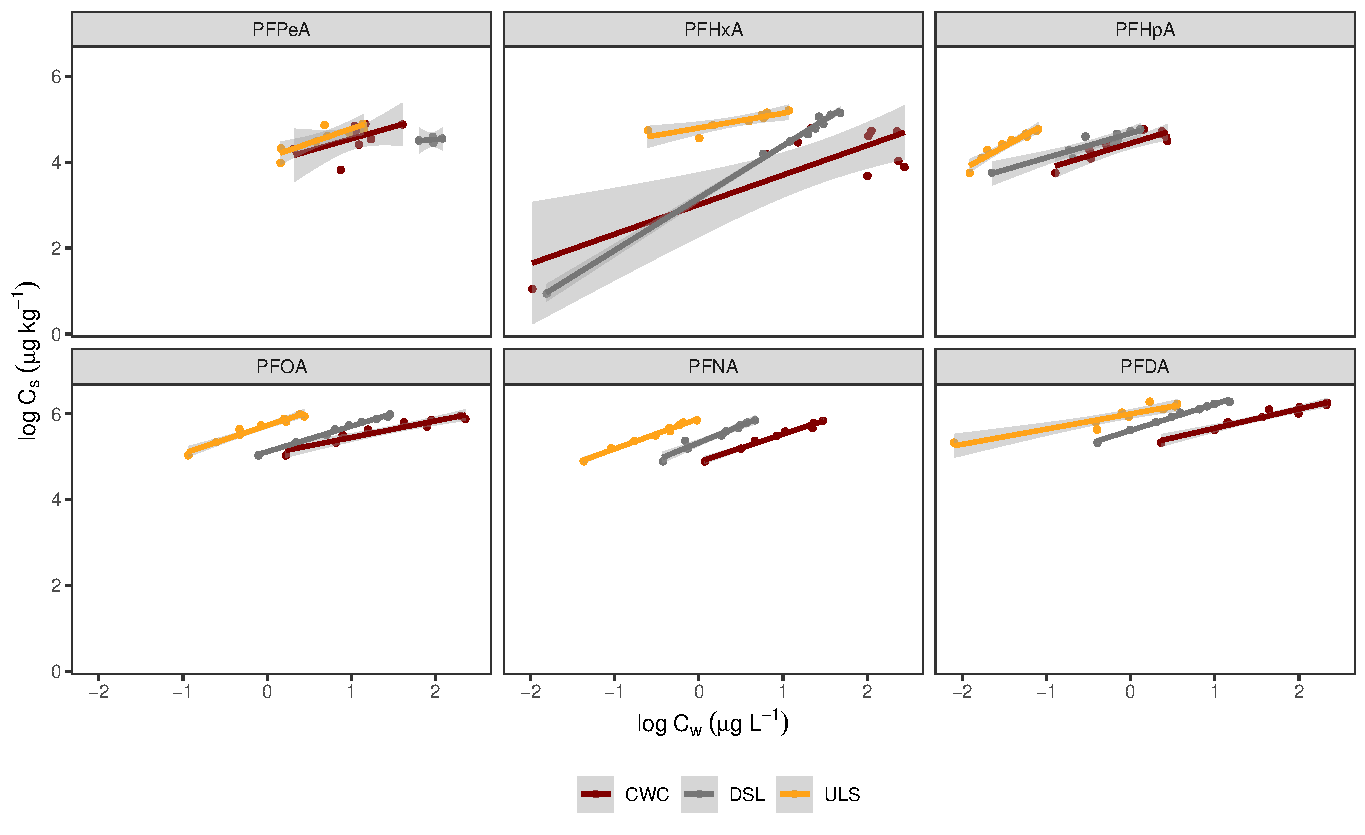
\includegraphics[width=\textwidth]{R/figs/Sorption_isotherms_single_BC.pdf}
    \caption{Freundlich sorption isotherms for PFPeA, PFHxA, PFHpA, PFOA, PFNA and PFDA in batch tests with three different biochars. Lines are obtained by linear regression.}
    \label{fig:sorption_isotherms}
\end{figure}

\begin{table}
\caption{Freundlich sorption coefficients and linear regression statistics for the BC-single isotherms in CWC, ULS and DSL (n=9). The error is presented as standard error. All $K_F$ data are in units of $\mathrm{(\mu g/kg)/(\mu g/L)^{n_F}}$.}
\centering
\adjustbox{max width=\textwidth}{%
\begin{threeparttable}
\label{tab:summary_stats_single}
\begin{tabular}{lllllllllllll} \toprule
PFCA & \multicolumn{4}{c}{ULS} & \multicolumn{4}{c}{DSL} & \multicolumn{4}{c}{CWC} \\ \cmidrule(l){2-5} \cmidrule(l){6-9} \cmidrule(l){10-13}
 & $\log~K_{F,BC}$ & $n_{F,BC}$ & $r^2$ & $p$ & $\log~K_{F,BC}$ & $n_{F,BC}$ & $r^2$ & $p$ & $\log~K_{F,BC}$ & $n_{F,BC}$ & $r^2$ & $p$ \\ \midrule
PFPeA & 4.10 ± 0.13 & 0.67 ± 0.16 & 0.74 & ** &  &  &  & $>$0.05 &  &  &  & $>$0.05 \\
PFHxA & 4.80 ± 0.06 & 0.34 ± 0.09 & 0.72 & ** & 3.30 ± 0.15 & 1.11 ± 0.11 & 0.93 & *** &  &  & & $>$0.05 \\
PFHpA & 5.98 ± 0.17 & 1.08 ± 0.11 & 0.93 & *** & 4.67 ± 0.06 & 0.57 ± 0.09 & 0.86 & *** & 4.44 ± 0.05 & 0.59 ± 0.11 & 0.80 & ** \\
PFOA & 5.73 ± 0.02 & 0.65 ± 0.05 & 0.95 & *** & 5.12 ± 0.02 & 0.60 ± 0.02 & 0.99 & *** & 5.06 ± 0.08 & 0.39 ± 0.05 & 0.90 & *** \\
PFNA & 5.89 ± 0.02 & 0.71 ± 0.03 & 0.99 & *** & 5.33 ± 0.03 & 0.80 ± 0.07 & 0.94 & *** & 4.88 ± 0.04 & 0.65 ± 0.04 & 0.98 & *** \\
PFDA & 6.00 ± 0.04 & 0.35 ± 0.05 & 0.86 & *** & 5.61 ± 0.02 & 0.61 ± 0.02 & 0.99 & *** & 5.22 ± 0.07 & 0.45 ± 0.04 & 0.94 & *** \\ \bottomrule
\end{tabular}
\begin{tablenotes}
\item Significance codes: *** $<$ 0.001, ** $<$ 0.01
\item Insignificant regressions (p $<$ 0.05) have been removed
\end{tablenotes}
\end{threeparttable}}
\end{table}

\subsection{Effects of PFCA physicochemical properties on sorption}
\begin{landscape}


\begin{figure}[tb]
    \centering
    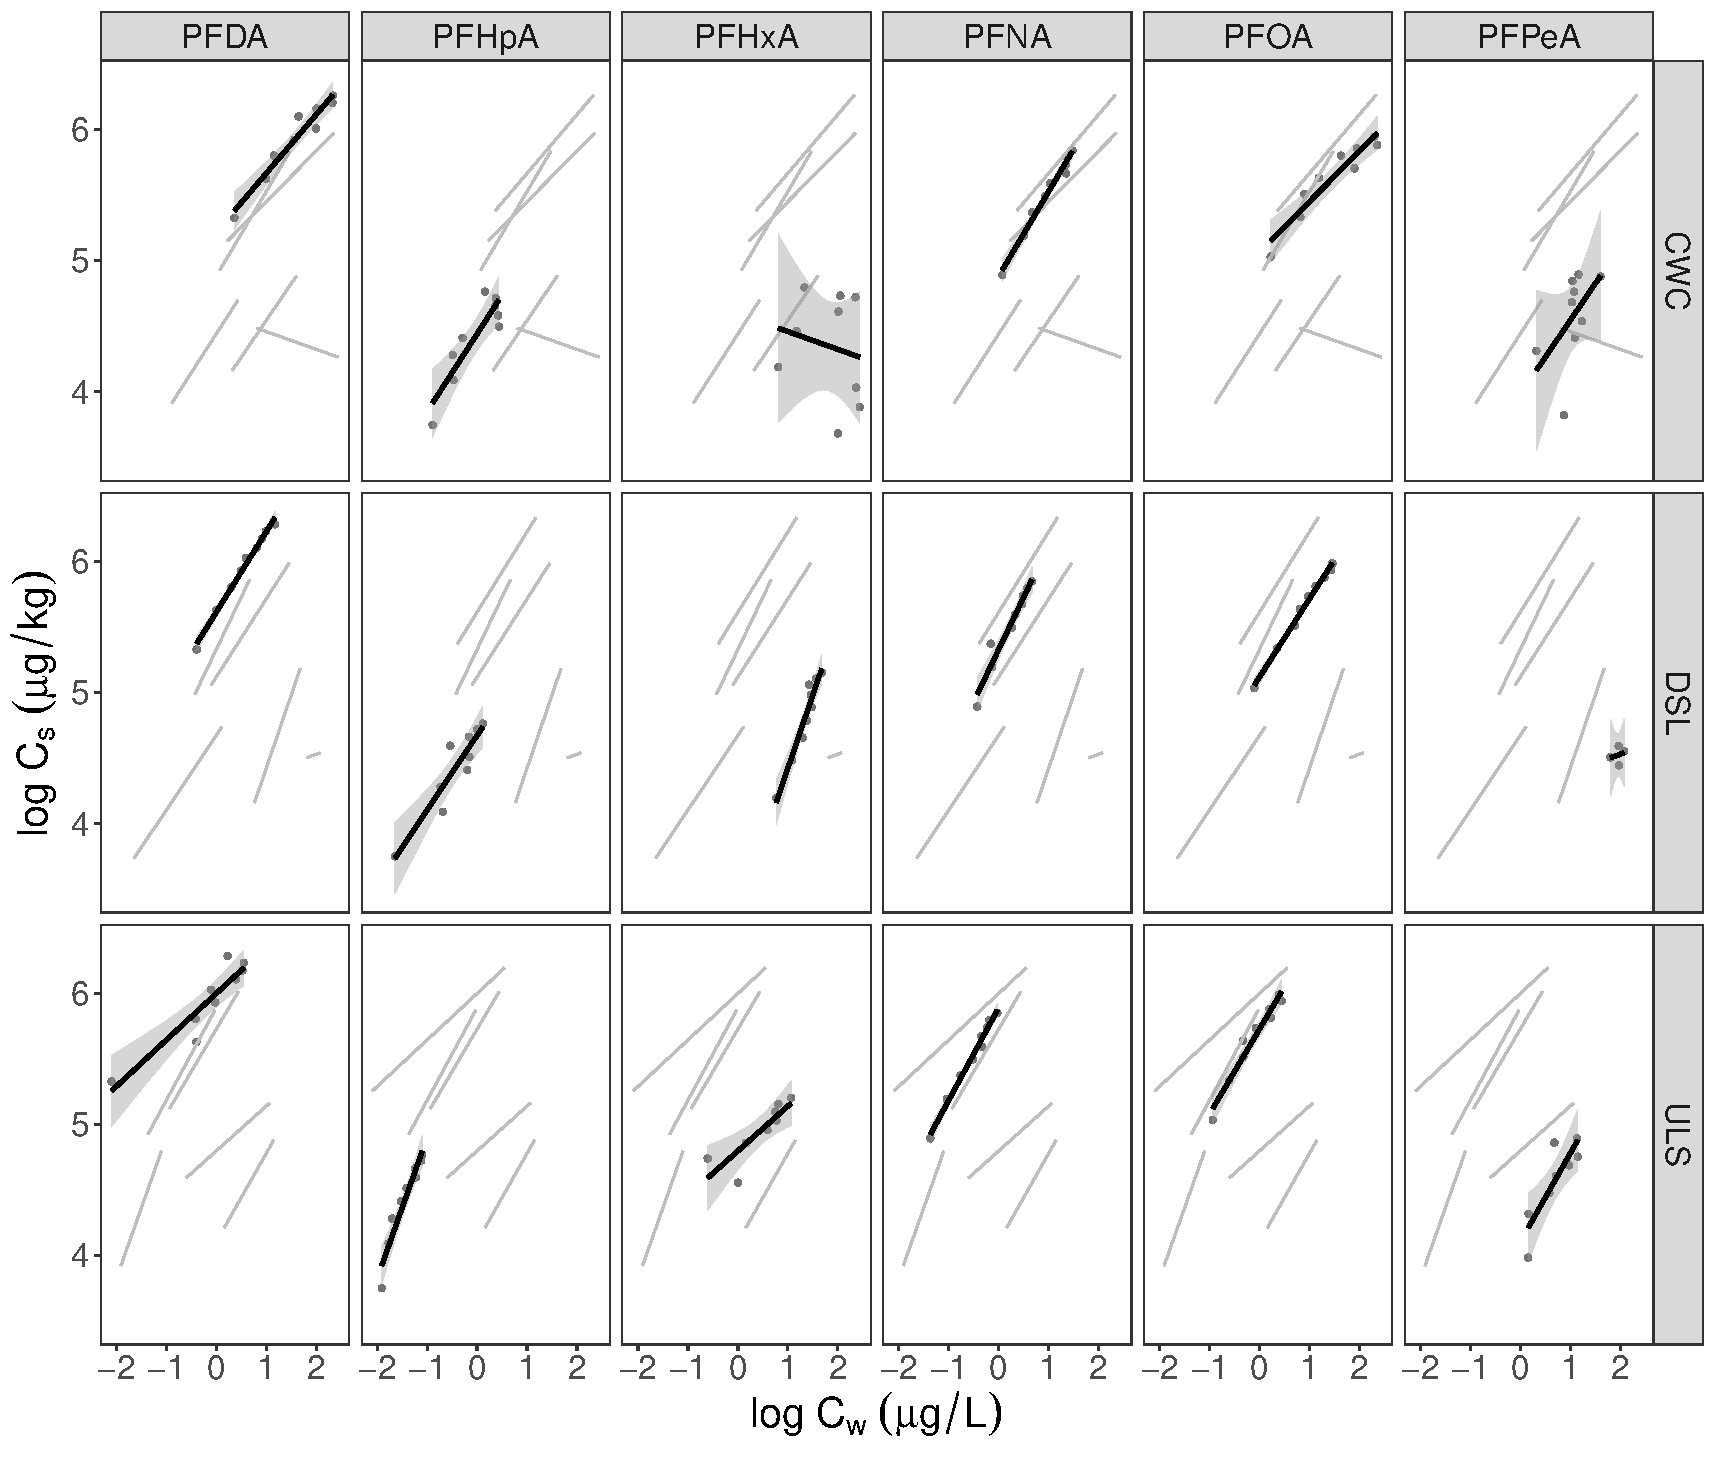
\includegraphics[height=0.8\textheight]{R/figs/BC_facet_isotherm.pdf}
    \caption{Single-compound Freundlich sorption isotherms for PFPeA, PFHxA, PFHpA, PFOA, PFNA and PFDA. Lines are obtained by linear regression. For comparison across chain length, the shaded gray lines are the isotherms from the other compounds with the same sorbent.}
    \label{fig:sorption_isotherms_all}
\end{figure}

\end{landscape} 
\subsubsection{Effects of PFCA chain length}
\Cref{fig:sorption_isotherms_all} shows sorption isotherms for the single-compound batch tests for CWC, ULS and DSL. The Freundlich coefficients ($\log~K_F$) reported are in units of $\mathrm{(\mu g/kg)/(\mu g/L)^{n_F}}$. Sorption to ULS increased in the order: PFPeA (CF4) $<$ PFHxA (CF5) $<$ PFOA (CF7) $<$ PFHpA (CF6) $<$ PFNA (CF8) $<$ PFDA (CF9) where $\log~K_F$ ranged from 4.10$\pm$0.13 to 6.00$\pm$0.04 . Sorption to DSL increased in the order: PFHxA (CF5) $<$ $<$ PFHpA (CF6) $<$ PFOA (CF7) $<$ PFNA (CF8) $<$ PFDA (CF9) where $\log~K_F$ ranged from 3.30$\pm$0.15 to 5.61$\pm$0.02. Sorption to CWC increased in the order: PFPeA (CF4) $<$ PFHpA (CF6) $<$ PFHxA (CF5) $<$ PFNA (CF8) $<$ PFOA (CF7) $<$ PFDA (CF9), where $\log~K_F$ ranged from $\log~K_F$ 3.98$\pm$0.36 to 5.22$\pm$0.07. Insignificant ($p>0.05$) isotherms have not been reported. Poor correlations for the isotherm regressions were achieved for the short-chain PFCAs (PFPeA, PFHxA, and PFHpA) when sorption isotherms were derived. This can be attributed to poor sorption affinity to biochar. All Freundlich coefficients are listed in \cref{tab:summary_stats_single}. 

The sorption of PFAS increased with greater fluorinated chain length. A statistically significant relationship between $\log~K_F$ and CF\textsubscript{2} chain length was found for all three biochars (p$<$0.05) to PFOA, PFNA, and PFDA (\cref{fig:chainlength}) in accordance with previous studies \citep{Sorengard2019, fabregat2022examining, ahmed2020per}. There was a difference of 1.2-1.9 $\log~K_F$ units between the longest and the shortest PFCA chain (PFDA and PFPeA). This relationship suggests that hydrophobic interactions play a major role in sorption. For every CF\textsubscript{2} moiety, hydrophobic interactions between condensed aromatic structures in the biochar matrix increases, contributing to stronger sorption. 

Several mechanisms can explain why perfluorinated carboxylic acids increase in hydrophobicity with increasing chain length: 1) Due to a high molecular surface of the perfluorinated tail, a high cavity formation energy is needed to dissolve the compounds in water \citep{Arp2006}. For this reason, the compounds tend to be pushed towards water-solid interfaces, such as a biochar surface. For this reason, dissolution becomes decreasingly entropically favorable as chain length increases\citep{sigmund2022sorption}. 2) Compared to a hydrocarbon chain, the perfluorinated chain is capable of the lowest van der Waals dispersive forces per molecular surface area \citep{du2014adsorption}. The result is that PFAS has a much weaker attraction to water molecules when these are in the water cavity than hydrophobic organic compounds. For this reason, PFASs are both oil- and water repellent.  Generally, water cavity formation energy and van der Waals interactions have been considered insignificant for sorption of short-chain PFAS to solid phases (\textless C6) \citep{du2014adsorption}. They are, however, significant for long-chained PFCs (\textgreater C6) \citep{du2014adsorption} which corresponds with the chain length dependency found in this study.

\begin{figure}[tbh]
    \centering
    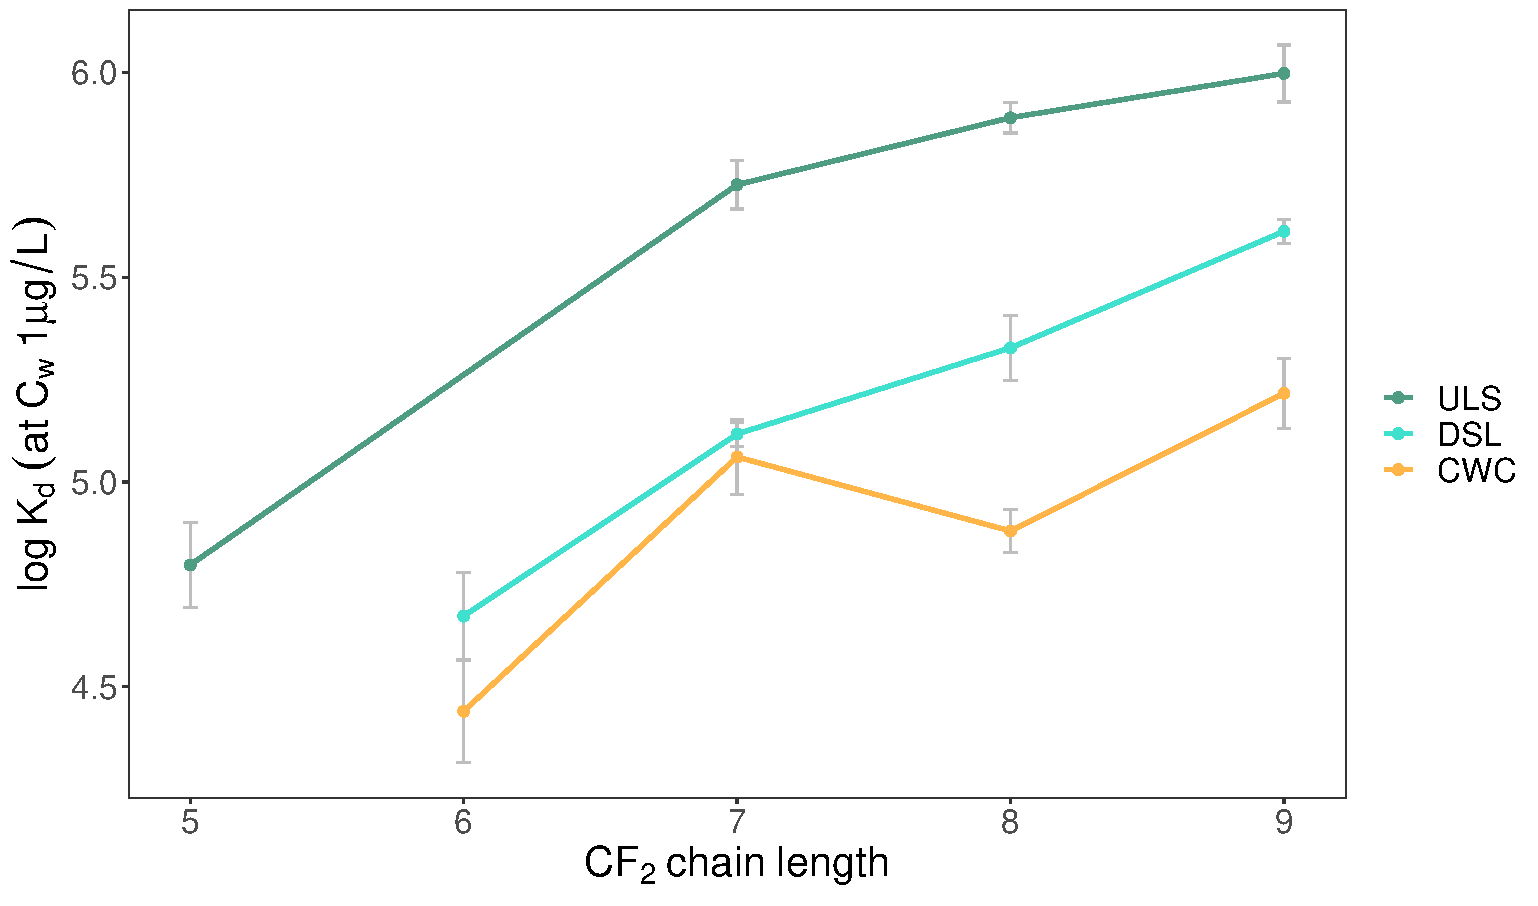
\includegraphics[width=0.7\textwidth]{R/figs/chain_length_Kd1ugL_plot.pdf}
    \caption{Relationship between $\log~K_F$ and chain length. Linear regression coefficients for ULS: $r^2$ = 0.92, $p$ = 0.04, DSL: $r^2$ = 0.98, $p$ = 0.01, CWC: $r^2$ = 0.68, $p$ = 0.17. Error bars are the propagated error of $\log~K_F$ and $n_F$.}
    \label{fig:chainlength}
\end{figure}

\subsubsection{PFAS functional groups} 
With the positive correlation between chain-length and PFCA sorption found in this study (\cref{fig:chainlength}), electrostatic interactions by the negatively charged carboxylate functional group seem to be of lesser importance. However, the effect of the charge-assisted polar head, especially for short-chain PFAS, cannot be disregarded. PFAS can engage simultaneously in hydrophobic interactions (perfluorinated chain) and in electrostatic interactions (attraction and repulsion), with both surface functional groups and dissolved ions (head) \citep{zhang2013sorption,sigmund2022sorption}. The different electrostatic interactions (cation bridging, biochar surface attraction and repulsion) are discussed more in depth in \cref{sec:inorganic}.

\cite{zhang2021sorption} found that sorption increased in the order PFBA $<$ PFBS $<$ PFOA $<$ PFOS for granular activated carbon and softwood-derived biochar. The difference between the PFSA and PFCA groups is that PFSAs have one more perfluorinated carbon than PFCAs, which have their terminal carbon bonded as a carboxylate (COO\textsuperscript{-}) instead of an additional $\mathrm{CF_2}$ moiety. If one compares PFHpS to PFOA, which both have the same number of $\mathrm{CF_2}$ moieties, perfluorinated sulfonic acid still sorbs better. Researchers attribute this to: 1) A difference in molecular size because the sulfonate moiety is slightly larger than the carboxylate moiety. This results in a greater cavity formation energy for PFSAs. Hence, in water saturated conditions, the functional group is pushed towards water extremities \citep{yin2022insights,sigmund2022sorption}. In batch shaking experiments, the water extremities would be the biochar surfaces or labware. 2) Sulfonic acid is a stronger acid than carboxylic acid. This results in a stronger ionic interaction to positive charges of mineral phases in biochar ash \citep{arvaniti2015review}. 

%%%%%%%%%%%%%%%%%%%%%%%%%%%%%%%%%%%%%%%%%%%%%%%%%%%%%%%%%%%%%%%%%%%%%%%%%%%%%%%%%%%%%%%%%%%%%%%%%%%%%%%%%%%%%%%%%%%%%%%%%%%%%%%%%%%%%%%%%%%%%%%%%%%%%%%%%%%%%%%%%%%%%%%%%%%%%%%%%%%%%%%%%%%%%%%%%%%%%%%%%%%%%%%%%%%%%%%%%%%%%%%%%%%%%%%%%%%%%%%%%%%%%%%%%%%%%%%%%%%%%%%%%%%%%%%%%%%%%%%%%%%%%%%%%%%%%%%%%%%%%%%%%%%%%%%%%%%%%%%%%%%%%%%%%%%%%%%%%%%%%%%%%%%%%%%%%%%%%%%%%%%%%%%%%%%%%%%%%%%%%%%%%%%%%%%%%%%%%%%%%%%%%%%%%%%%%%%%%%%%%%%%%%%%%%%%%%%%%%%%%%%%%%%%%%%%%%%%%%%%%%%%%%%%%%%%%%%%%%%%%%%%%%%%%%%%%%%%%%%%%%%%%%%%%%%%%%%%%%%%%%%%%%%%%%%%%%%%%%%%%%%%

\section{The effect of biochar properties on sorption}
In this section, the distribution coefficients derived for ULS, DSL and CWC biochars will be considered in relation to the following BC characteristics in an attempt to gain insight into possible sorption mechanisms: main elements (C, H, O, N), trace elements (Ca and Fe), surface area (\acrshort{SA}), and pore volume (\acrshort{PV}). In comparing sorbent properties and sorption coefficients for each biochar feedstock, PFOA, PFNA and PFDA have been used because they exhibited the best sorption isotherms. The Freundlich coefficients ($\log~K_F$) have been normalized to 1 $\mathrm{\mu g~L^{-1}}$ which is used as the distribution coefficient ($K_d$) in this discussion. Conducting multivariate analyses between biochar $K_d$ and the different supporting parameters for the biochar samples was desirable,  but not statistically valid due to there being no degrees of freedom with only 3 samples. Therefore, the discussion on the effects of biochar properties on sorption will be limited to discerning trends with SA, PV, C, Ca and Fe. 

\subsection{Surface area and pore volume}\label{sec:SAPV}

\begin{table}
\centering
\caption{Surface area (SA), pore volume (PV), element content (C, O, H, N), and ratios for the biochars evaluated in the laboratory experiments.}
\adjustbox{max width=\textwidth}{
\label{tab:SAPV}
\begin{tabular}{lcccccccccccc}
\toprule
Biochar & \multicolumn{2}{l}{N\textsubscript{2} sorption} & \multicolumn{2}{l}{CO\textsubscript{2} sorption} & \multicolumn{4}{l}{Elemental content} & \multicolumn{3}{c}{Element ratio} \\
sorbent & \multicolumn{2}{l}{(pores \textgreater 1.5 nm)} & \multicolumn{2}{l}{(pores 0.4-1.5 nm)} & & & & & & \\ \cmidrule(l){2-3} \cmidrule(l){4-5} \cmidrule(l){6-9} \cmidrule(l){10-12} 
& BET SA  & BJH PV  & DFT SA & DFT PV & C & O & H & N & O/C & H/C & N/C \\
& ($\mathrm{m^2~g^{-1}}$) & (cm\textsuperscript{3} g\textsuperscript{-1}) & ($\mathrm{m^2~g^{-1}}$) & (cm\textsuperscript{3} g\textsuperscript{-1}) & (\%) & (\%) & (\%) & (\%) & & & \\ \midrule
CWC & 323 & 0.017 & 683 & 0.186 & 91.4 & 5.50 & 1.01 & 0.69 & 0.06 & 0.01 & 0.008 \\
ULS & 128 & 0.126 & 165 & 0.047 & 29.6 & 57.1 & 1.24 & 1.13 & 1.9  & 0.04 & 0.04 \\
DSL & 110 & 0.111 & 87  & 0.027 & 13.5 & 61.4 & 1.05 & 0.82 & 4.6  & 0.08 & 0.06 \\ \bottomrule
\end{tabular}}
\end{table}

\subsubsection{Pore size distribution between 0.4-1.5 nm}
\cref{tab:SAPV} shows the total surface area (SA, m\textsuperscript{2}/g) and pore volume (PV, cm\textsuperscript{3}/g) for the three biochars used in the sorption experiments in this study. SA of CWC biochar (683 m\textsuperscript{2} g\textsuperscript{-1}) was $\sim$six times higher than that of ULS and DSL biochars (165 and 87  m\textsuperscript{2} g\textsuperscript{-1}, respectively), and PV followed the same pattern. Previous research has postulated that large internal surface areas and pore volumes are desirable for strong sorption of organic contaminants because they increase the fraction of active sorption sites \citep{ahmed2020per,Hale2016}. The high SA and PV of CWC suggests that this biochar has the highest fraction of active sites compared to ULS and DSL biochars within the micropore range ($\le$ 2 nm). However, for SA and PV, the pore size distribution (PSD) of pores available for CO\textsubscript{2} adsorption (0.4-1.5 nm), shown in \cref{fig:PZD_small}, makes clear that nearly 80\% of the SA, and 60\% of the PV of CWC biochar, are located in pores smaller than 0.6 nm. These are referred to as ultra micropores \citep{bardestani2019experimental}. To find out whether PFCAs can be absorbed into these ultra micropores, \cref{tab:molecsize} lists effective cross-sectional diameter ($D_{eff}$) and maximum diameter ($D_{max}$) of each PFCA (the definitions of $D_{eff}$ and $D_{max}$ are illustrated in \cref{fig:molecularSize}). PFCAs C5-C10 range from 0.45-0.72 nm ($D_{eff}$) to 0.96-1.54 nm ($D_{max}$). Since the respective perfluorinated chains are too large and rigid to enter, most pores ($<$ 0.6 nm) turned out to be inaccessible to the PFCA molecules \citep{yu2009sorption}. In addition, pores that are too small make it difficult for the compounds to adjust their shape to the pore walls in order to be able to come close enough to sorb to the biochar surface. This is why they can get stuck in a cross-sectional position that blocks the pores for diffusion of new sorbates. 

Maximum sorption is achieved when the molecular dimensions of PFAS match the pore size and shape of the sorbent \citep{Hale2016}. Since the \acrshort{PSD} within the CO\textsubscript{2}-range is dominated by ultra micropores, sorption of PFPeA, PFHxA, and PFHpA is only possible if the congeners enter the pores at the exact right angle. PFOA, PFNA, and PFDA will experience size exclusion as their molecules are too large to sorb into the biochar pores in any direction (\cref{tab:molecsize}). This means that sorption of PFAS in the CO\textsubscript{2}-range is insignificant, and cannot explain the differences in the $\log~K_F$ obtained for the biochar feedstocks, especially since strongest sorption was measured for long-chain PFCAs.

\begin{figure}[htb]
    \centering
    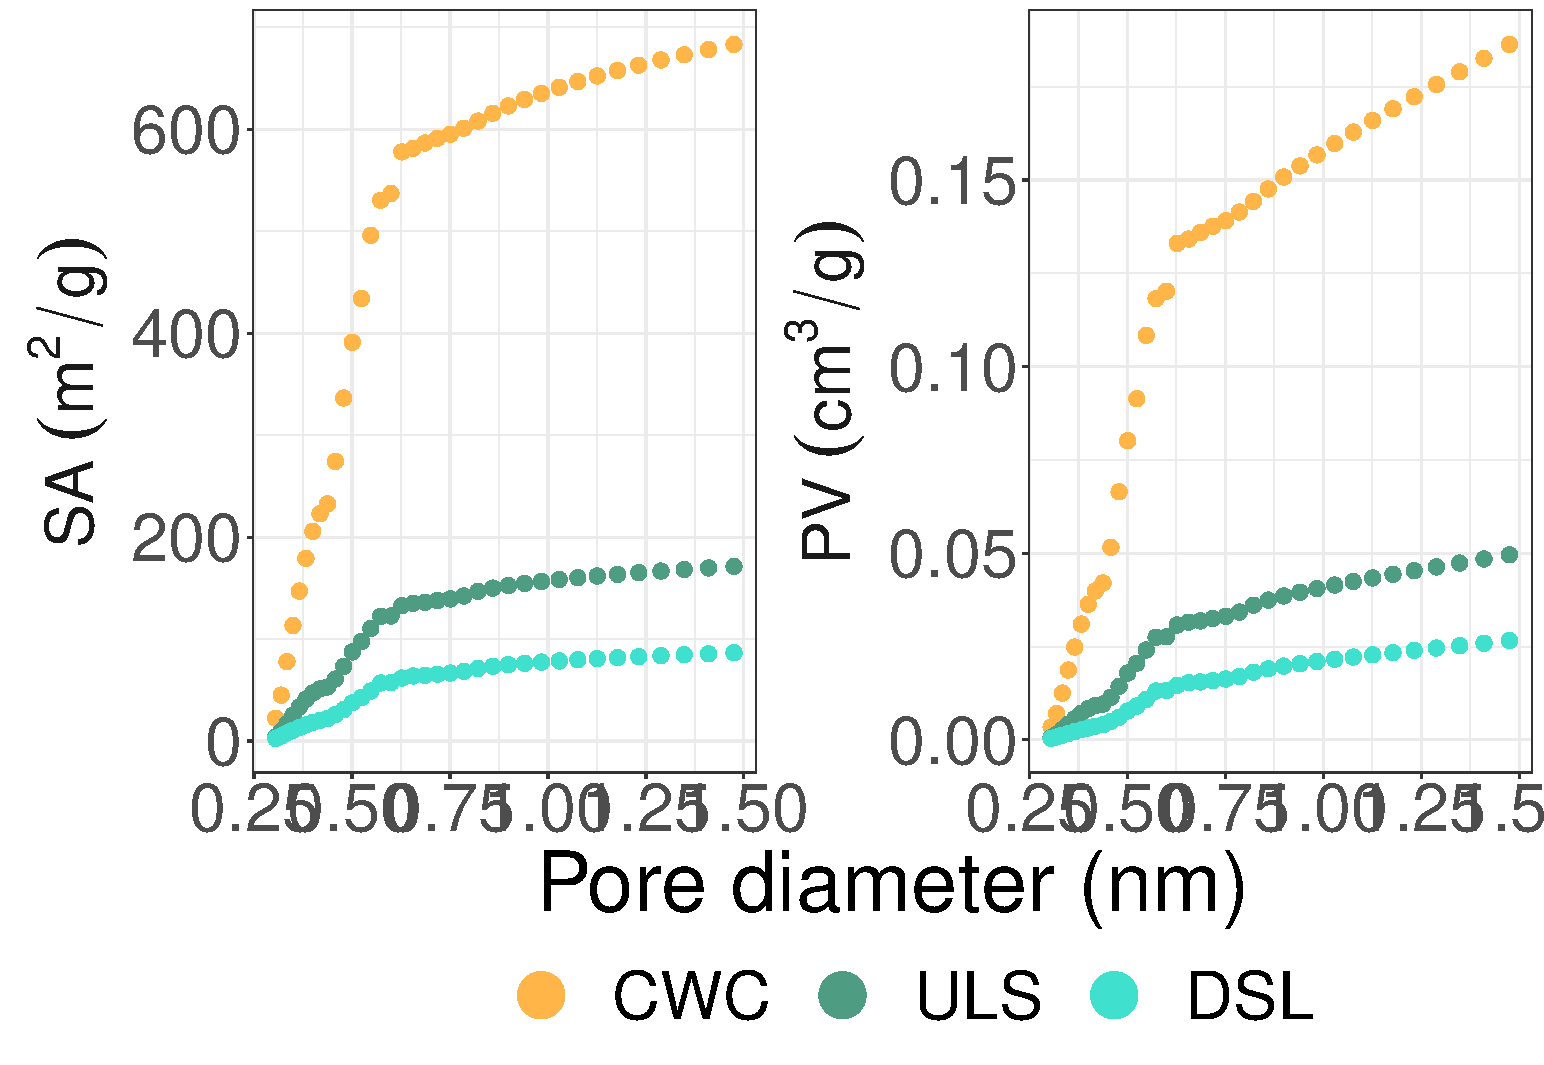
\includegraphics[width=\textwidth]{R/figs/PZD_SA_PV_small_plot.pdf}
    \caption{Cumulative pore size distribution for 0.4-1.5 nm-sized pores using DFT with (a) surface area (SA) and (b) pore volume (PV).}
    \label{fig:PZD_small}
\end{figure}

\begin{table}
\caption{Effective cross-sectional diameter ($D_{eff}$) and maximum diameter ($D_{max}$) of TCs interpolated and extrapolated by linear regression from calculations performed by \cite{inoue2012size} on PFOA and other PFCAs with chain lengths 11-18.}
\centering
\begin{threeparttable}
\label{tab:molecsize}
\begin{tabular}{lcrr}
\toprule
Compound & Chain & $D_{eff}$ & $D_{max}$ \\ 
& length & (nm) & (nm) \\ \midrule
PFPeA & 5  & 0.45  & 0.96  \\
PFHxA & 6  & 0.50  & 1.08  \\
PFHpA & 7  & 0.56  & 1.19  \\
PFOA\textsuperscript{*} & 8 & 0.61 & 1.36 \\
PFNA & 9 & 0.67 & 1.42  \\
PFDA & 10 & 0.72 & 1.54  \\ \bottomrule                                    
\end{tabular}
\begin{tablenotes}
\item \textsuperscript{*} Value from \cite{inoue2012size}
\end{tablenotes}
\end{threeparttable}
\end{table}

\begin{figure}
    \centering
    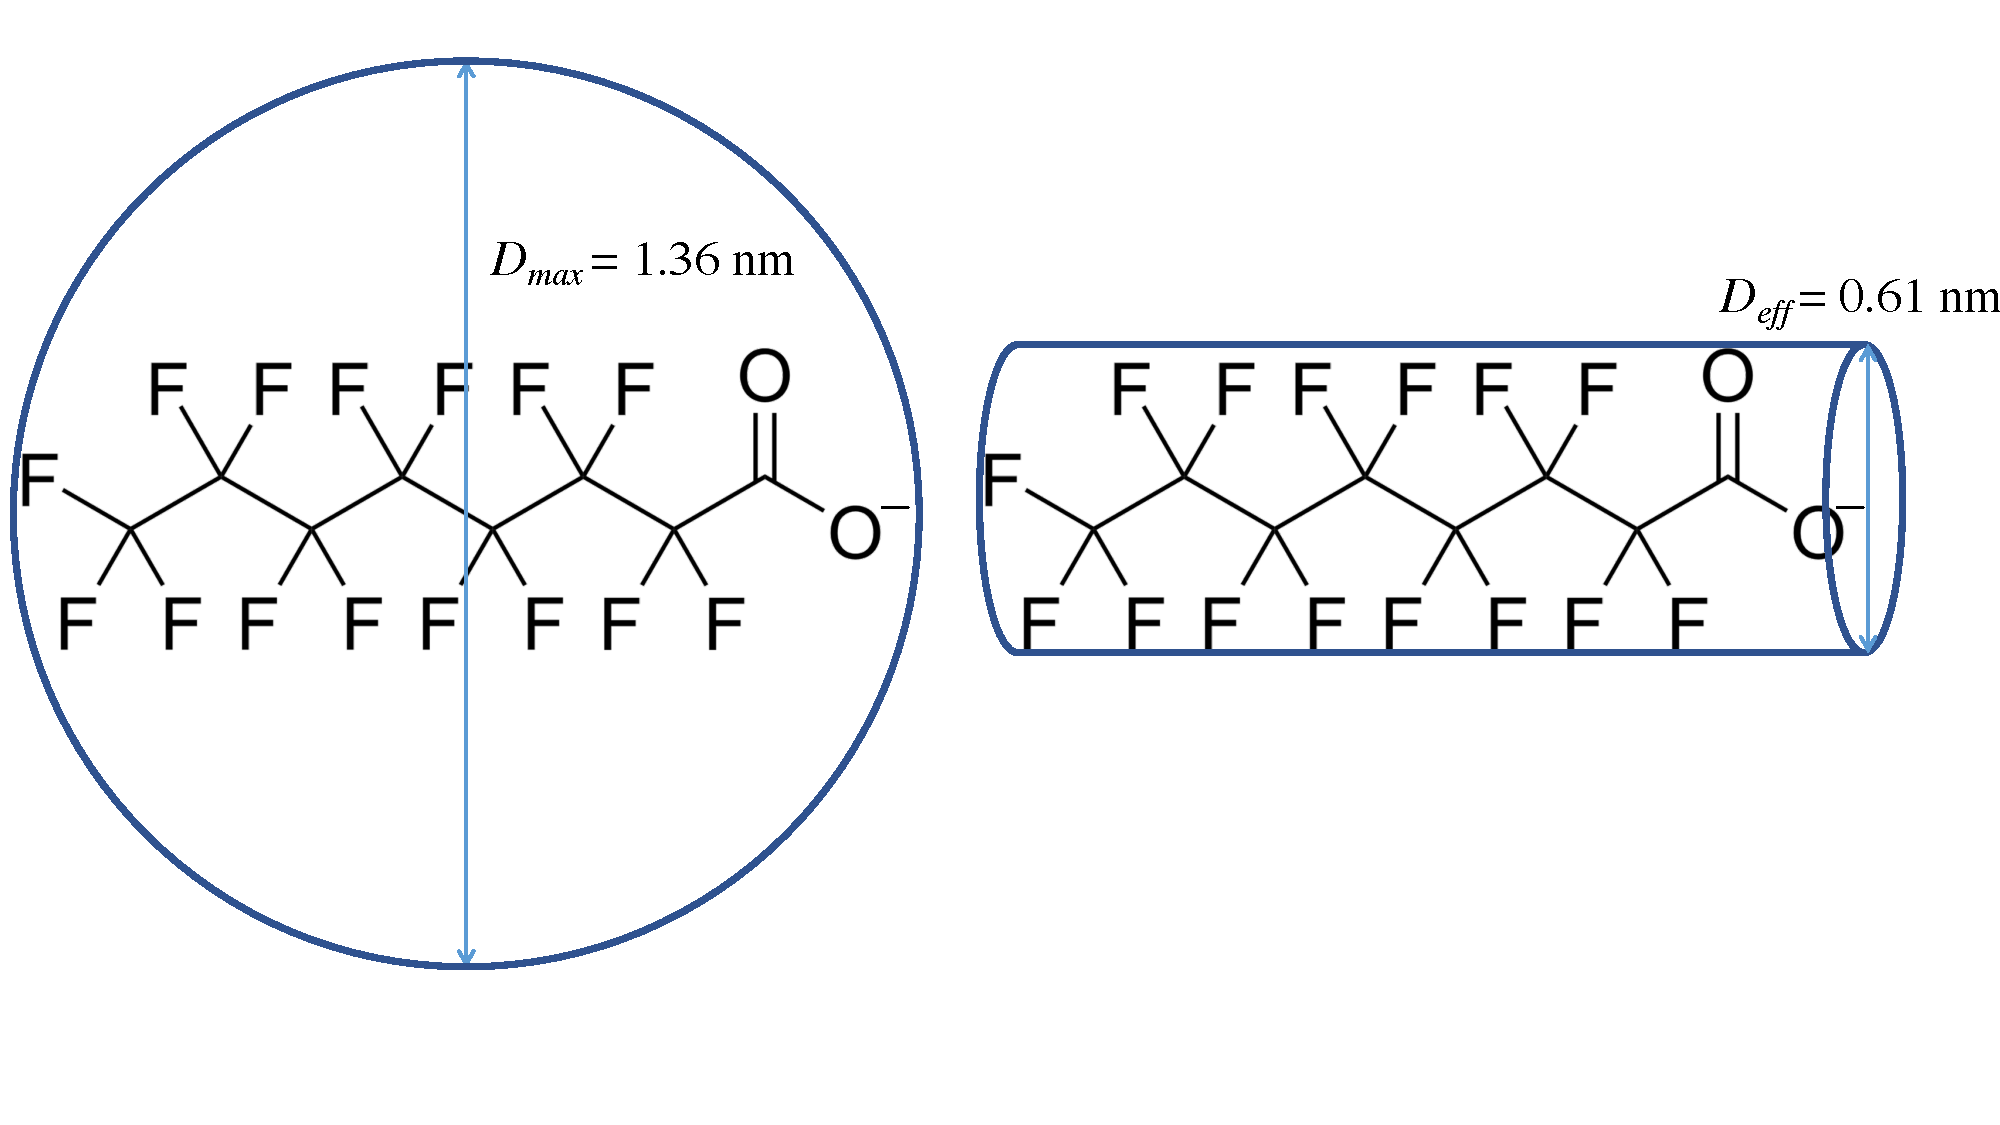
\includegraphics[width=0.8\textwidth, trim={0 2cm 0 0},clip]{Diagrams/Molecular_size.pdf}
    \caption{Effective cross-sectional diameter ($D_{eff}$) and maximum diameter ($D_{max}$) of PFOA.}
    \label{fig:molecularSize}
\end{figure}

\subsubsection{Pore size distribution for pores $>$1.5 nm}
CWC biochar had the largest cumulative SA (323 m\textsuperscript{2} g\textsuperscript{-1}), but the lowest PV (0.017 cm\textsuperscript{3} g\textsuperscript{-1}) for pores $>$1.5 nm. ULS biochar had slightly larger SA than DSL biochar (128 versus 110 m\textsuperscript{2} g\textsuperscript{-1}), as well as a slightly larger PV (0.126 versus 0.111 cm\textsuperscript{3} g\textsuperscript{-1}). In addition, the pore size distributions in \cref{fig:PZD_large} show remarkable differences in how SA and PV are distributed with increasing pore diameters between CWC biochar and the sludge biochars. For CWC biochar, SA and PV are almost exclusively allocated to pores between 1.5-3 nm. By contrast, SA and PV for the ULS and DSL biochars increase steadily up to a maximum pore size of 35 nm. Since ULS biochar has only slightly larger porosity compared to DSL biochar (\cref{fig:PZD_large}), the higher carbon content in ULS biochar (30 \% versus 14 \%) than DSL biochar indicates that more hydrophobic interactions are possible for ULS biochar. The difference in carbon content between ULS and DSL biochars is the most plausible explanation for why ULS biochar sorbs better than DSL biochar.. 

Apart from SA and PV, carbon content has, in previous literature, been a good predictor of sorption affinity to PFAS \citep{Hale2016, Cornelissen2005}. 

Three important conclusions can be drawn from this information: 1) CWC biochar has pores that are predominantly too small to accommodate PFCA, 2) CWC biochar has much lower PV for pores $>$1.5 nm, and this greatly restricts pore filling mechanisms, and 3) ULS biochar has a higher PV, SA and C-content than DSL biochar. This probably explains why ULS biochar is a better sorbent than DSL. In this study, the most plausible explanation for why CWC biochar is the weakest sorbent among the three biochars is that CWC biochar consists almost exclusively of micropores, whereas the ULS and DSL biochars have many more pores in the mesopore range (2-50 nm). This means that high porosity, and sufficiently large pores, are the two most important parameters that regulate high sorption capacity, and that a carbon-rich pore wall enhances sorption by increasing hydrophobic interactions. 

\begin{figure}[htb]
    \centering
    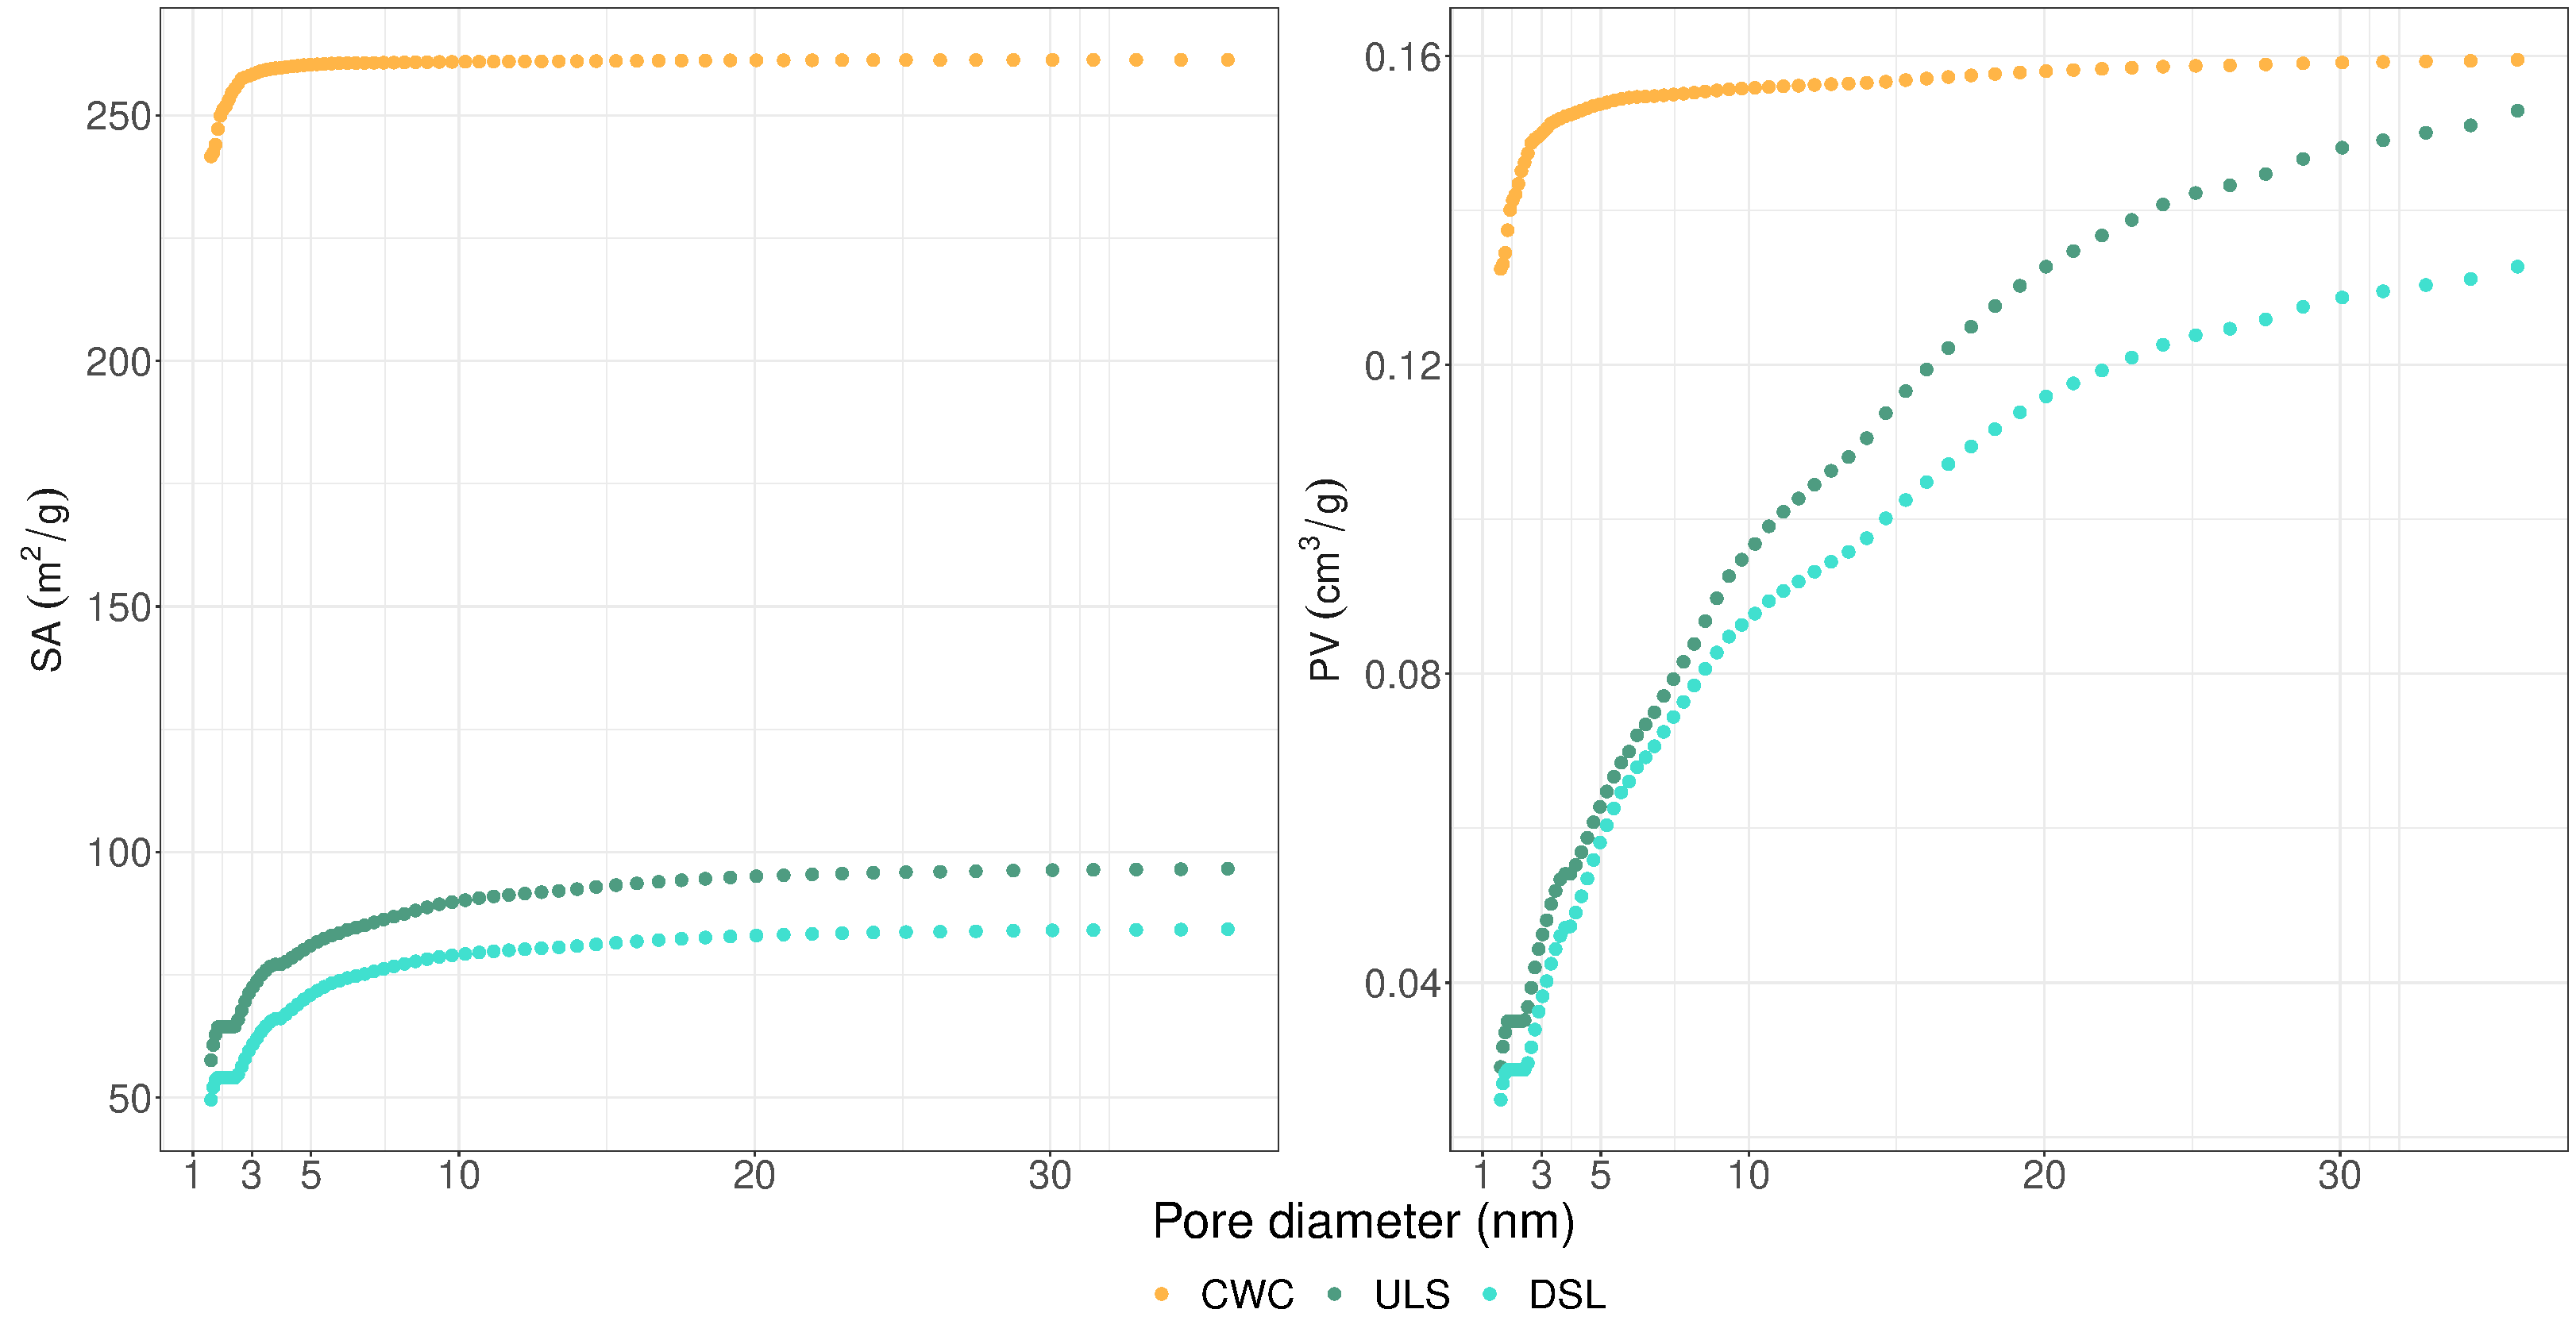
\includegraphics[width=\textwidth]{R/figs/PZD_SA_PV_plot_large.pdf}
    \caption{Cumulative pore size distribution for pores $>$ 1.5 nm using DFT theory with (a) surface area (SA) and (b) pore volume (PV).}
    \label{fig:PZD_large}
\end{figure}

\subsection{Biochar surface chemistry}
A higher carbon fraction is commonly used as an indicator of biochar aromaticity and, thereby, gives biochar a higher possibility for hydrophobic interactions \citep{Cornelissen2005}. The higher sorption of PFCAs to the ULS and DSL biochars stand in contrast to findings in previous literature that consistently report that higher C-content is a good predictor for increased sorption \citep{fabregat2022examining}. However, previous PFAS sorption studies have been conducted on activated biochar and charcoal, more carbon-rich and porous feedstocks than biochar from sewage sludge \citep{Sormo2021, zhang2021sorption}. Despite lower carbon contents in the ULS and DSL biochars, this study supports previous literature that concluded that the importance of electrostatic interaction to sorption is secondary to the hydrophobic effect. 

Surface hydrophobicity and degree of carbonization can be described by O/C, H/C, and N/C ratios \citep{chun2004compositions}. As reported previously, the O/C ratio of CWC (0.06) is within the same range as non-activated biochars pyrolyzed at 700\textdegree C \citep{LehmannAndJoseph2015, chun2004compositions,kupryianchyk2016biochar}. By contrast, the high oxygen content of DSL and ULS (61.4 and 57.1 \% respectively) results in increased O/C ratios of 4.6 and 1.9 respectively (\cref{tab:SAPV}). The difference between the O/C ratio \textless 1 for CWC compared to ratios \textgreater 1 for ULS and DSL indicate a significantly different degree of carbonization between the two feedstock types. At the same time, H/C ratios for all three biochar feedstocks are similar, and are within the same range reported in previous literature \citep{chun2004compositions,kupryianchyk2016biochar}. 

A higher O/C and N/C ratio---indicative of more polar functional groups (hydroxyl, carbonyl, metal-containing groups, amines and amides)---has proven to be beneficial for PFAS sorption \citep{du2014adsorption,fabregat2022examining}. Researchers suggest several mechanisms related to surface polar groups that may contribute to enhanced sorption. First, basic functional groups such as amines have high $pK_a$s and are protonated at environmentally relevant pH levels, providing anion exchange capacity and electrostatic attraction to the carboxylic acid heads \citep{deng2010removal}. Basic sites in \textpi-electron-rich, carbon-rich materials are important for PFAS sorption \citep{saeidi2020understanding}. N/C ratios for ULS and DSL are one order of magnitude higher than CWC. A high nitrogen/carbon (N/C) ratio can be indicative of more amine groups in the periphery of the condensed carbon structure. The positive charge on the nitrogen-containing functional groups can interact electrostatically with the PFCA carboxylate group. In addition, it is possible that they also engage in weak non-specific electrostatic interactions with the negative dipole of the CF-chain \citep{xiao2011effects}. The latter mechanism could explain the positive chain-length dependency on sorption seen for the sewage sludge biochars (\cref{fig:chainlength}), in addition to the low SA/PV/C ratio discussed in the previous section. Sewage sludge contains a homogeneous mixture of proteins and inorganic nutrients that will denaturate in some form during thermal treatment. To the author's knowledge, no data exists on how speciation of nitrogen changes during pyrolysis. Even though a higher N/C ratio is only an indication for nitrogen functional groups, the presence of amines is likely.

\begin{table}
\centering
\caption{Mean pH ($\pm$ standard error) measurements for the different batch test slurries (n=3) where S is soil and BC/S/L is the biochar:soil:liquid ratio.}
\label{tab:pHcond}
\begin{tabular}{lcc}
\toprule
Biochar & \multicolumn{1}{c}{pH} & BC/S/L\\ \midrule
ULS   & 7.10 ± 0.03 & 1/0/500\\
DSL   & 7.31 ± 0.01 & 1/0/500\\
CWC   & 7.36 ± 0.04 & 1/0/500\\
ULS+S & 7.18 ± 0.01 & 1/50/500\\
DSL+S & 7.14 ± 0.00 & 1/50/500\\
CWC+S & 7.09 ± 0.03 & 1/50/500\\
S     & 7.08 ± 0.03 & 0/1/10\\
\bottomrule
\end{tabular}
\end{table}


\subsubsection{Solution and biochar surface chemistry \label{sec:inorganic}} 
Solution chemistry, pH, and the composition of elements other than C, O, H and N, may provide further insight into how the pore walls of CWC, ULS and DSL differ from one another, as well as how these elements can influence sorption. pH varied little across sample types with an average pH of 7.18 $\pm$ 0.02 (\cref{tab:pHcond}). Therefore, pH levels for the biochar-water batch tests slurries have only been used to discuss expected surface charges. In the environment, the carboxylic functional group of PFCAs is negatively charged due to the strong electron-withdrawing fluorine atoms \citep{goss2008pKa}. Surface charges for biochar are pH-dependent, and are usually negatively charged at a neutral pH \citep{zhang2013sorption}. This was the case for the batch tests in the present study. However, point-of-zero charge measurements for the biochars did not become available in time for incorporation in this discussion. Therefore, a net negative biochar surface is assumed, but not confirmed \citep{saeidi2020understanding}.

In this study, highest sorption was seen for the biochars that had the highest composition of elements other than C, O, H, and N. CWC biochar contained only 1.4\% of other elements, whereas the sludge biochars, ULS and DSL, contained substantially more (10.9\% and 23.2\% respectively). A table with the total biochar elemental composition is given in \cref{appSec:elements}. Some of these elements are commonly found as freely dissolved ions. Since dissolved ions were not analyzed, we can only assume that, by and large, the alkalis (K and Na), and earth alkalis (Mg and Ca), are present as dissolved cations that originate from the biochar ashes. It is likely that Fe is predominantly incorporated in the biochar matrix. Iron speciation will be further discussed in \cref{sec:Fe}. The higher content of other elements than C, H, O, and N in ULS and DSL biochars suggests that sorption of PFCAs onto the sludge chars were likely influenced by the presence of charged species, both in the solution, as well as on the biochar surface. Coexisting inorganic ions complicate the sorption behavior of PFCAs because sorption can both be suppressed and enhanced by different electrostatic mechanisms \citep{du2014adsorption}. This will be discussed below. 

Sorption can be suppressed by electrostatic repulsion of the carboxylate group on PFCA by the negatively charged biochar surface, or by competitive sorption of anions to positive BC sites \citep{sigmund2022sorption}. Electrostatic repulsion explains why $K_F$-values were lowest for the shorter-chain PFCAs (\cref{tab:summary_stats_single}). The repulsion effect becomes weaker for the longer-chain PFCAs where the hydrophobic effect become more dominant. Electrostatic repulsion is reduced at lower pH because more negative BC sites are protonated, a process called surface-charge neutralization \citep{zhang2013sorption}. This allows for PFCA anion- \textpi-bond interaction with biochar \citep{sigmund2022sorption}. Sorption can be enhanced through electrostatic attraction to positively charged BC functional groups, and by divalent cation bridging \citep{du2014adsorption}. Cation bridging is the electrostatic linking of negatively charged PFCAs to negatively charged biochar surfaces by means of a divalent ion that acts as a "bridge" between them \citep{sigmund2022sorption}. Ca\textsuperscript{2+} and Mg\textsuperscript{2+} are common divalent ions present in biochar ash that contribute to bridging. The composition of Ca\textsuperscript{2+} and Mg\textsuperscript{2+} was three to six times higher in the sludge biochars when compared to CWC biochar (\cref{tab:BC_mainElements}. 

Bridging has been shown to be an important sorption mechanism in, for example, sediments, mineral materials, and black carbon \citep{higgins2006sorption}. Apart from bridging between the BC surface and PFAS functional groups, divalent ions can chain individual PFAS molecules together \citep{wang2011}. This creates an even more hydrophobic complex that can sorb more strongly to biochar. For this reason, more frequent formation of divalent cation bridges for the ULS and DSL biochars is expected. Although sorption \textit{capacity} has not been measured directly, the above mechanisms for PFAS interaction with charged and polar functional groups may be contributors to the higher sorption found for the more heterogeneous, mineral-rich matrices of sewage sludge biochars.

In this study, the positive correlation between $\log~K_F$ and chain length for all three biochars (\cref{fig:chainlength}) indicates that electrostatic interactions play a minor role for sorption to these biochars. If electrostatic interactions played an equally important role as hydrophobic interactions, sorption across differing PFCA chain lengths would be more similar. 

\begin{table}
\centering
\caption{Composition of a selection of elements in the biochar samples in g/kg.}
\label{tab:BC_mainElements}
\begin{tabular}{lrrrrrrrr} \toprule
 & Ca & Fe & K & Mg & Na & P & S & Si \\ \midrule
CWC & 8 & 0.1 & 4.0 & 0.9 & 0.05 & 0.4 & 0.09 & 0.2 \\
DSL & 26 & 180 & 3.7 & 4.7 & 1.8 & 8.0 & 7.2 & 0.6 \\
ULS & 21 & 23 & 6.8 & 5.3 & 2.4 & 45 & 2.9 & 1.7 \\ \bottomrule
\end{tabular}
\end{table}

\subsubsection{Iron speciation\label{sec:Fe}}
Due to a lack of corresponding reference compounds for some of the EXAFS signals, no satisfying fit was obtained for the iron species present in sewage sludge biochar samples. This suggests that iron is not only present as iron oxides. The Fe K-edge XANES spectra (\cref{appFig:valence}) and EXAFS spectra (\cref{appFig:Fe_species}) show that DSL and ULS are similar in valence and speciation. They consist mainly of reduced forms of Fe (Fe(II)), and DLS is slightly more reduced than ULS. Total Fe concentration is especially high for DSL (180 mg/kg, \cref{tab:BC_mainElements}), making up as much as 18\% of its matrix (3.3\% and 0.01\% for ULS and CWC respectively). The Fe concentration will therefore significantly affect the surface morphology of DSL. PFAS has been shown to form inner-sphere complexes via covalent metal-ligand bonds (Fe-carboxylate) by means of the following reaction \citep{du2014adsorption}:

\begin{equation}
    \mathrm{\equiv Fe-OH_2^+ ~ + ~ CF_3(CF_2)_nCOO^- \rightarrow ~ \equiv Fe-OOC(CF_2)_nCF_3 ~+~ H_2O}
\end{equation}

The triple bond represents chelation of Fe to the biochar matrix. Point of zero charge (PZC) for Fe(oxyhydr)oxides, such as ferrihydrite and goethite, are around 7, similar to the solution pH measured for the water-biochar systems (see \cref{sec:inorganic}). The iron species are expected to be neutral for the systems analyzed, and will likely not be one of the dominating sorption mechanisms for PFCA. 

%%%%%%%%%%%%%%%%%%%%%%%%%%%%%%%%%%%%%%%%%%%%%%%%%%%%%%%%%%%%%%%%%%%%%%%%%%%%%%%%%%%%%%%%%%%%%%%%%%%%%%%%%%%%%%%%%%%%%
%%%%%%%%%%%%%%%%%%%%%%%%%%%%%%%%%%%%%%%%%%%%%%%%%%%%%%%%%%%%%%%%%%%%%%%%%%%%%%%%%%%%%%%%%%%%%%%%%%%%%%%%%%%%%%%%%%%%%
%%%%%%%%%%%%%%%%%%%%%%%%%%%%%%%%%%%%%%%%%%%%%%%%%%%%%%%%%%%%%%%%%%%%%%%%%%%%%%%%%%%%%%%%%%%%%%%%%%%%%%%%%%%%%%%%%%%%%

\section{Sorption attenuation by soil and PFCA cocktail}
This section discusses sorption attenuation for the different batch test categories that were prepared (\cref{fig:batchtests_flowchart}). The categories are: 

\begin{itemize}
    \item \textbf{BC-single}: biochar-water spiked with single PFCAs
    \item \textbf{BC-mixed}: biochar-water spiked with a PFCA cocktail
    \item \textbf{BC-soil-PFOA}: soil-biochar-water spiked with single PFOA only
    \item \textbf{BC-soil-mixed}: soil-biochar-water spiked with a PFCA cocktail
    \item \textbf{Soil-single}: soil-water spiked with single PFCAs
    \item \textbf{Soil-mixed}: soil-water spiked with a PFCA cocktail
\end{itemize}

\Cref{subfig:C10} shows how much $K_d$ is suppressed by the presence of soil and/or a mixture of PFCAs at the highest spike point, SC10. A description of considerations that were taken for the determination of $K_d$ values in soil is in \cref{appSec:Sorption}, \cref{appsec:attenuation}. The difference in $\log~K_d$ between BC single and the other sample types is directly related to how much sorption was attenuated by the presence of soil and/or other PFCAs. As visualized by the order of the colored points, attenuation increased in the following order: BC-single (reference) $>$ BC-soil-single $>$ BC-mixed $\sim$ BC-soil-mixed $>$ soil-single and soil-mixed. Attenuation factors ($AF$) were calculated for each category:

\begin{equation} \label{eq:$AF$}
    AF = \frac{K_{BC-single}}{K_{BC-x}}
\end{equation}

where $K_{BC-single}$ is the expected sorption, and $K_{BC-x}$ is the measured partition coefficient for the mixed, soil-mixed, or soil-single batch tests. In \cref{subfig:$AF$}, the $AFs$ for PFOA, PFNA, and PFDA have been plotted for each biochar. $AFs$ ranged from 3-10 for BC-S-PFOA, 6-140 for BC-mix, and 8-138 for BC-S-mix (\cref{tab:attenuation}). The cocktail consisted of 18\% PFOA, 21\% PFNA, and 49\% PFDA (\cref{tab:spikeConcentrations}). Since the concentrations for each compound was different, and nearly 50\% of the cocktail was PFDA, PFNA and PFOA, likely were overwhelmed, showing that PFDA  a trend for attenuation with chain length cannot be derived. These factors are very high due to five other compounds added at similar concentrations with a total concentration of 10 mg/L. It was difficult to evaluate any trends in $AF$s between biochar samples or PFCA chain lengths, but PFDA does not seem to be overwhelmed... 

Since the $AFs$ varied widely within each category, mean and median values for each category were calculated to evaluate trends. BC-S-PFOA: mean = 6, median = 4, BC-mix: mean = 43, median = 29, and BC-S-mix: mean = 59, median = 49. Thus, attenuation for the cocktail samples was one to two orders of magnitude higher than attenuation by soil alone. The presence of soil with a cocktail caused additional attenuation of 27\% ($\mathrm{AF_{soil} = 59-43 = 16}$. These $AFs$ are in the same range as in previous literature where it was established that sorption was attenuated by a factor of 10 for phenanthrene by means of adding other PAHs \citep{Cornelissen2006}, 32 for a mixture of DDT \citep{hale2009sorption}, and 100-500 for sulfamethazine (SMT) in soil after \cite{Teixido2013}. The high attenuation for sulfamethazine seen by \cite{Teixido2013} is in the same order as the $AFs$ found in the present study. Sorption of both SMT (a structure  that consists of a sulfonamide functional group that links two aromatic rings with nitrogen-substitutions, methyls and an amine), and PFAS to biochar seems to be more affected by the presence of soil than does sorption of the hydrophobic organic contaminants (HOCs), phenanthrene and DDT. Though speculative, and taking into account that sorbents and conditions vary, this could indicate that HOCs can more easily penetrate the humic acid pore blockages than can PFAS and SMT. A hypothesis that could explain this is that SMT and PFAS are more similar in hydrophobicity as humic acids. This means that they share a level playing field in the competition for sorption sites. However, since humus is larger than PFAS, pores remain non-penetrable. A more extensive determination of structure-property relationships and attenuation would be needed to confirm this hypothesis. 

As a final note, one cannot know if the $AFs$ derived after 14 days in the present study would be reduced given increased soil-BC-mix and BC-water-mix contact times such as were seen by \cite{hale2009sorption} who found that attenuation of DDT disappeared ($AF$ = 1) after 26 months. A sorption capacity test would have to be conducted to determine if sorption sites for CWC, ULS, and DSL biochars truly were saturated and at equilibrium after 14 days for BC-mix without soil. Or whether diffusion and occupation of all sorption sites would increase with increased contact time. 

To the best of the author's knowledge, there are no existing attenuation factors for sewage sludge biochar to PFAS. Attenuation depends mainly on two factors: 1) sediment-BC contact time, and 2) concentration of cocktail. Since it was shown that soil did not contribute to further suppressed sorption, sorbents can, without difficulty, be amended to soil with low TOC (1.3\%), such as the present one \citep{Sormo2021}.


\begin{table}
\centering
\caption{Attenuation factors ($AF$) calculated as $K_{BC_single}/K_{BC_x}$ and respective $\log~K_d$-values at SC10.}
\label{tab:attenuation}
\begin{tabular}{llrrrrrr} \toprule
Compound & type & \multicolumn{2}{c}{CWC} & \multicolumn{2}{c}{DSL} & \multicolumn{2}{c}{ULS} \\ \cmidrule(l){3-4} \cmidrule(l){5-6} \cmidrule(l){7-8}
 &  & $\log~K_d$ & $AF$ & $\log~K_d$ & $AF$ & $\log~K_d$ & $AF$ \\ \midrule
PFOA & BC-mix & 2.84 & 6 & 3.17 & 23 & 4.13 & 29 \\
PFNA & BC-mix & 2.33 & 109 & 3.03 & 140 & 4.40 & 29 \\
PFDA & BC-mix & 2.95 & 9 & 3.60 & 32 & 5.09 & 9 \\ \addlinespace \hline \addlinespace
PFOA & BC-S-mix & 2.73 & 8 & 3.24 & 19 & 3.47 & 134 \\
PFNA & BC-S-mix & 2.68 & 48 & 3.33 & 71 & 3.73 & 138 \\
PFDA & BC-S-mix & 2.91 & 10 & 3.67 & 27 & 4.16 & 78 \\ \addlinespace \hline \addlinespace
PFOA & BC-S-PFOA & 3.19 & 3 & 3.98 & 4 & 4.61 & 10 \\ \bottomrule
\end{tabular}
\end{table}


\begin{figure}
    \centering
        \begin{subfigure}[]{\linewidth}
            \centering
            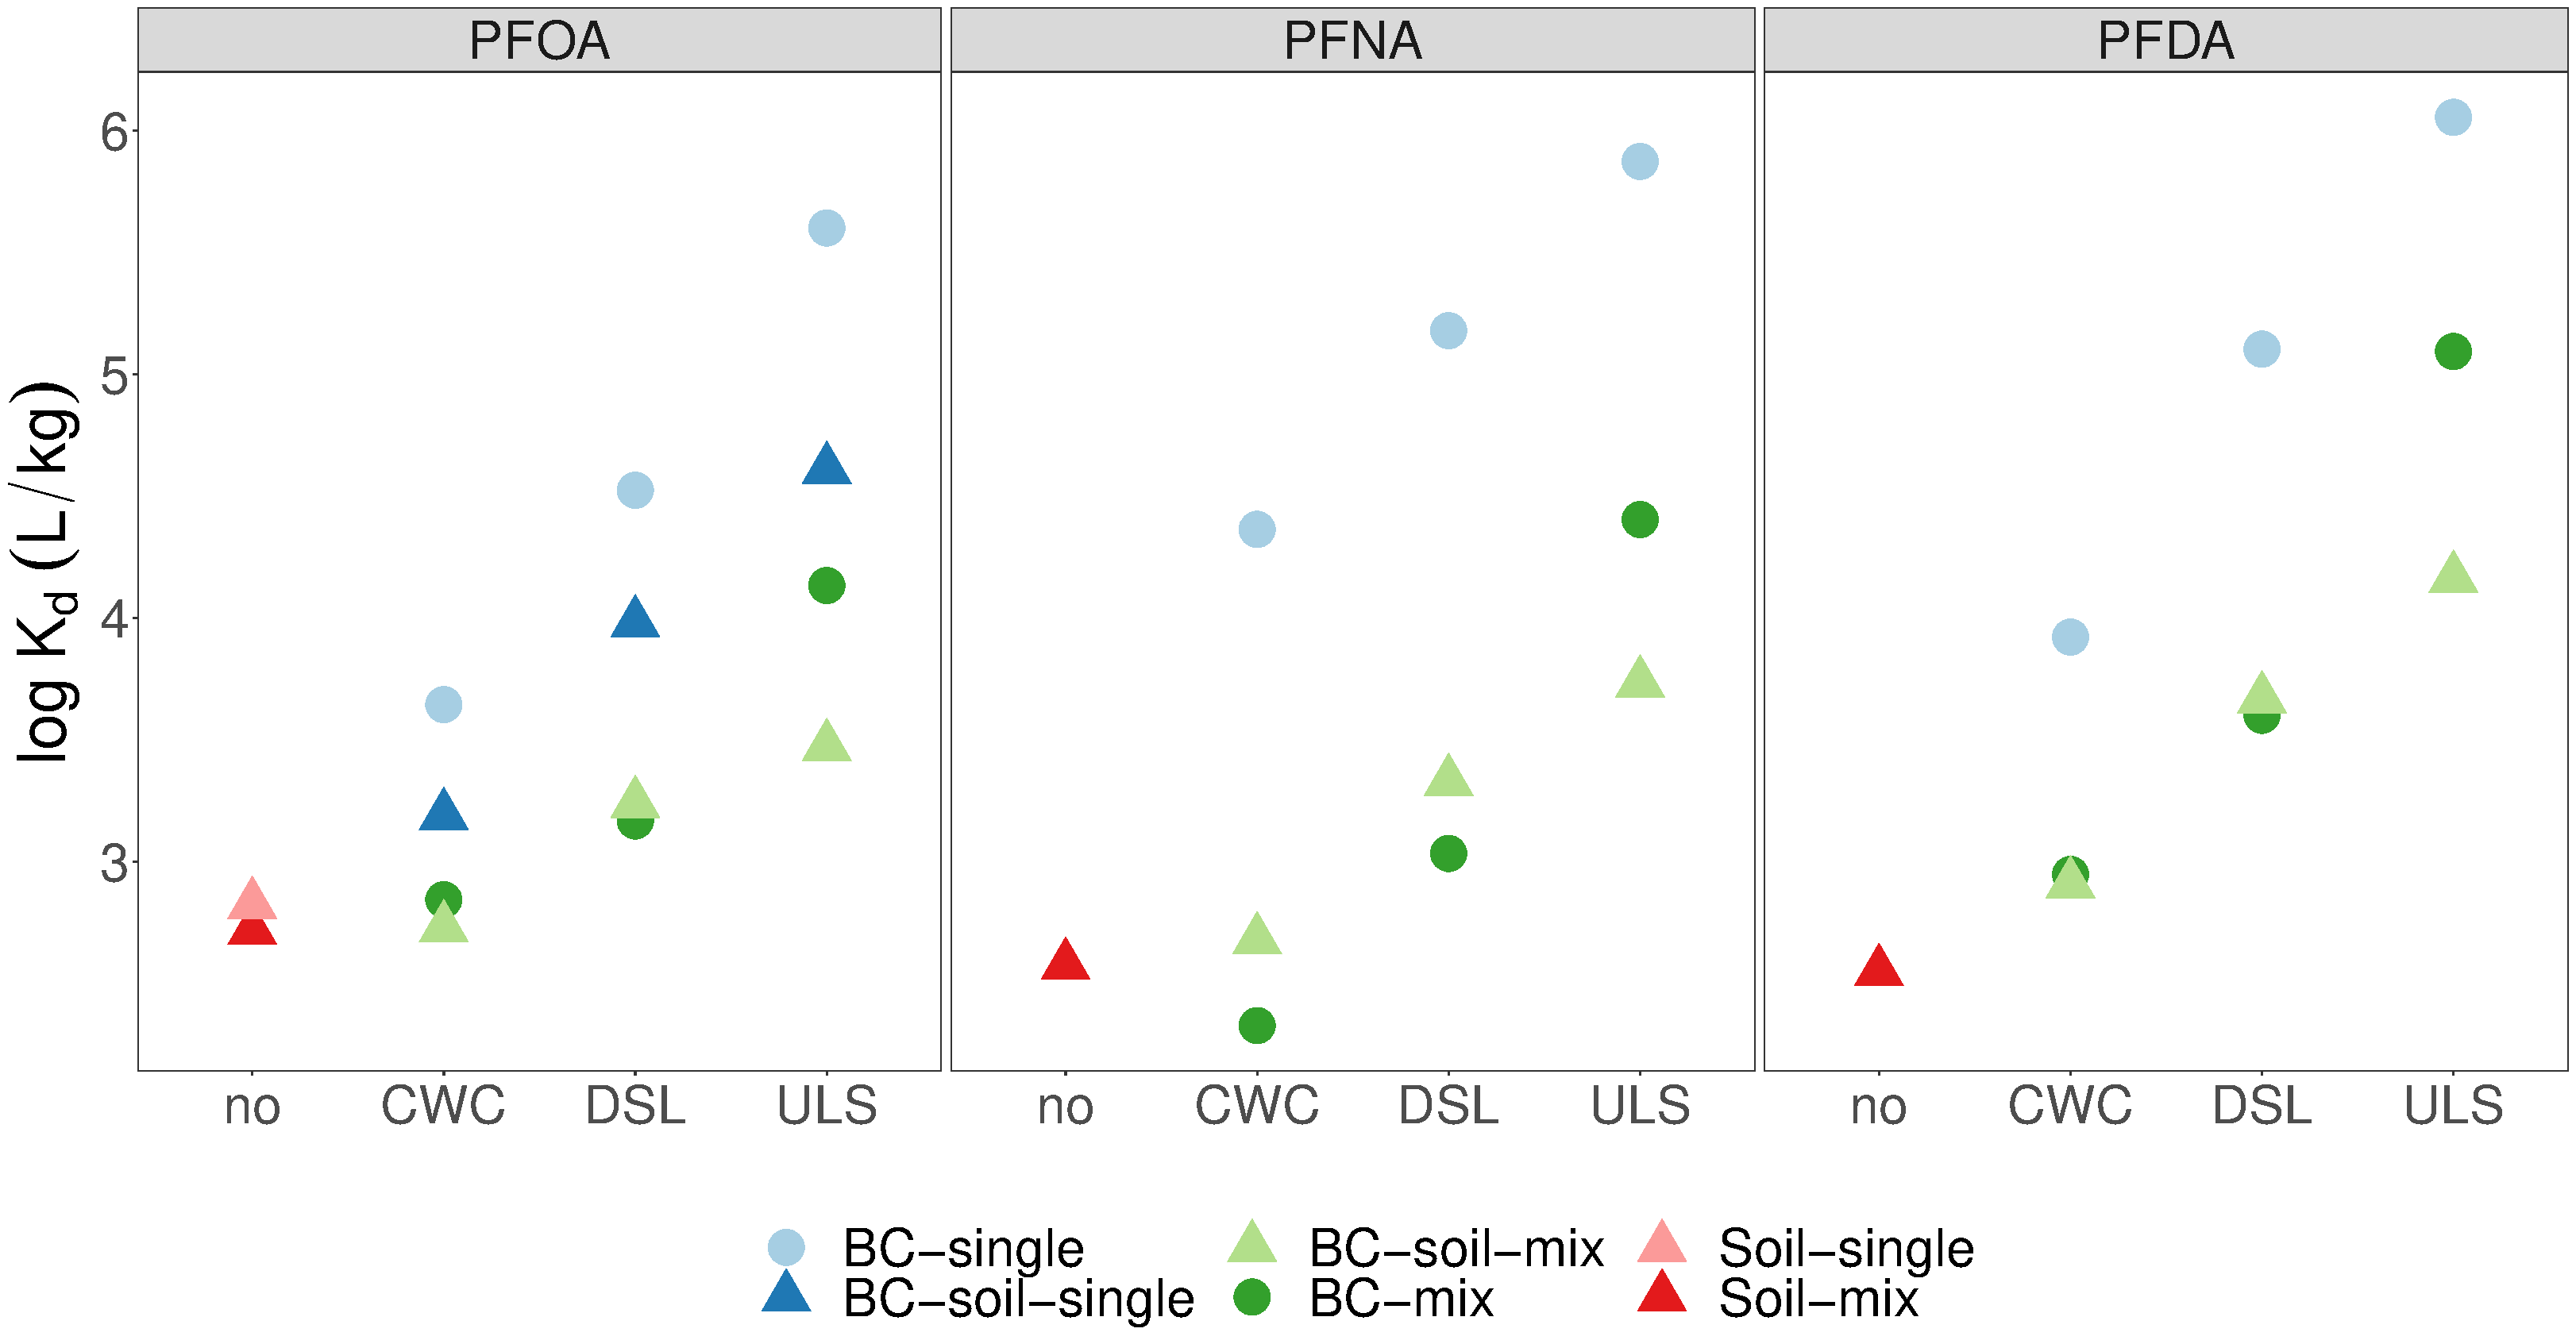
\includegraphics[width=0.75\textwidth]{R/figs/C10.pdf}
            \subcaption{$\log~K_d$ for PFOA, PFNA, and PFDA spiked at SC10 (1 953, 1 409, and 3 830 \textmu g L\textsuperscript{-1} respectively) for the different biochar feedstocks (CWC, DSL, ULS) and soil-only (no biochar). $\log~K_d$ for BC single (light blue circles) are the predicted sorption by biochar.}
            \label{subfig:C10}
        \end{subfigure}
        \begin{subfigure}[]{\linewidth}
            \centering
            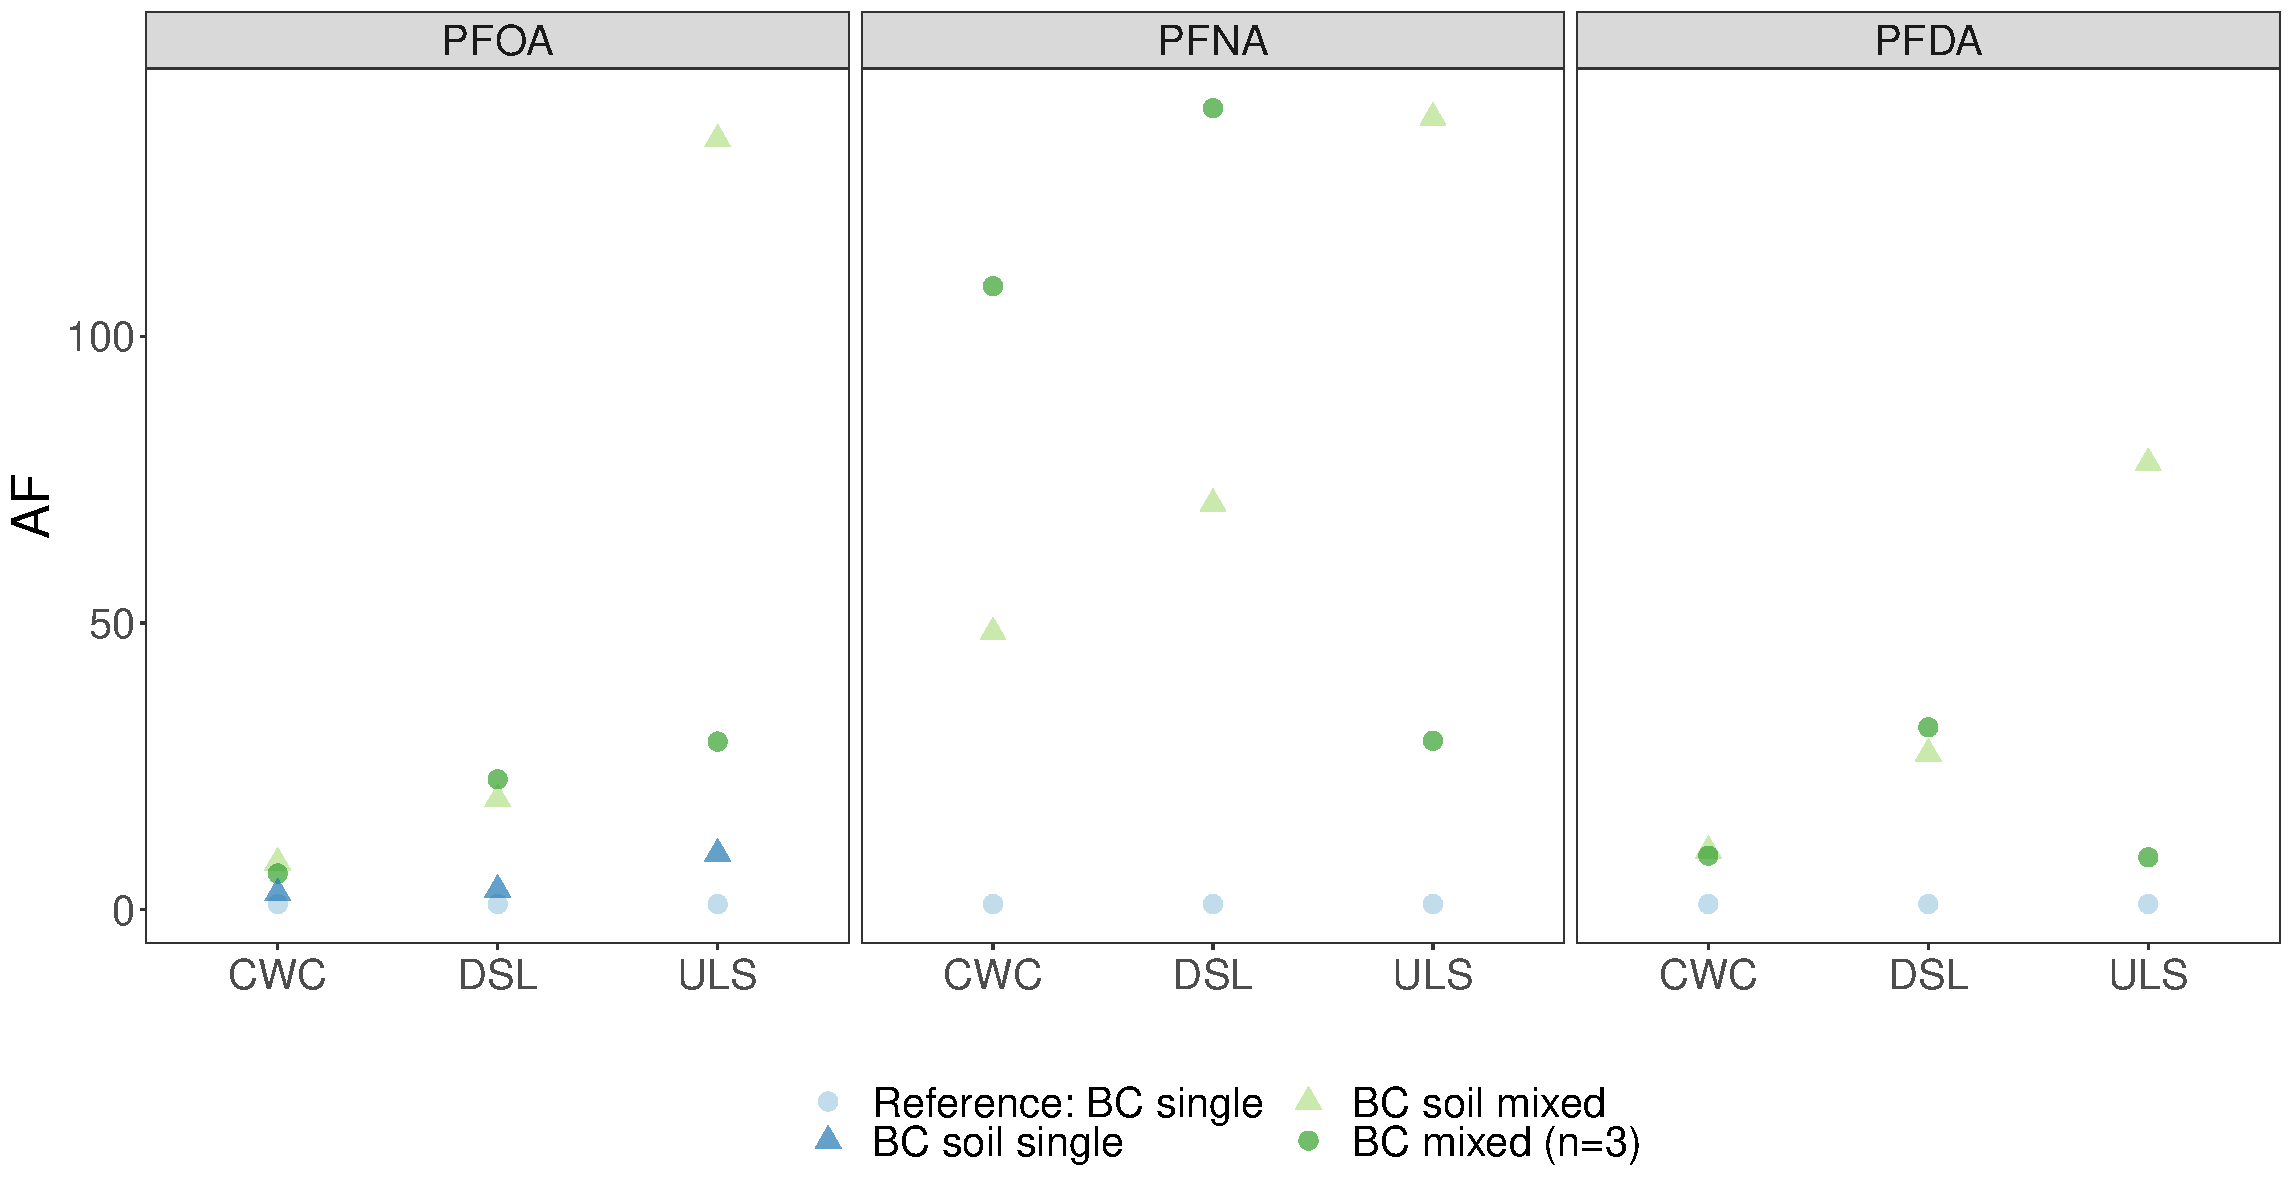
\includegraphics[width=0.75\textwidth]{R/figs/Attenuation_factors_C10_OND.pdf}
            \subcaption{Attenuation factors ($AF$) at SC10 for PFOA, PFNA, and PFDA calculated as $K_{d,BC single}/K_{d,x}$ where $K_{d,x}$ are batch test categories. See \cref{tab:spikeConcentrations} for spike concentrations used for each PFCA in the single-spike and cocktail-spike batch tests.}
            \label{subfig:$AF$}
        \end{subfigure}  
    \caption{Reduction in \textbf{(a)} $\log~K_d$ at SC10 and \textbf{(b)} attenuation factors at SC10.}
    \label{fig:C10_AF}
\end{figure}

\subsection{Sorption attenuation of PFOA isotherms}
\cref{fig:PFOA_attenuation} shows the effect of attenuation on the PFOA isotherms for BC soil single, and BC soil mixed. The isotherms were spiked with the same $C_i$ as BC single. But only six of the ten points were selected for the attenuation isotherms (\cref{sec:S-BC}. For all biochars, BC single has the highest sorption, followed by BC soil single, and BC soil mixed. This trend gives a good indication of the order of factors that influence attenuation, and is consistent with the results discussed in the previous section. The isotherms have similar $C_s$ concentrations, but varying $C_w$, depending on sample type. Due to pore blocking and competitive sorption by natural organic matter and natural compounds, more sorbate in solution is needed to push the same number of molecules onto the solid phase in the presence of soil, an effect that can be further enhanced by the presence of both soil and a cocktail since this isotherm has the highest $C_w$ and lowest $C_s$. This particular quality is due to the fact that PFCAs with longer chain lengths (PFNA and PFDA) have an advantage over PFOA when competing for sorption sites \citep{Sormo2021}. Supported by the trends in \cref{fig:C10_AF}, the cocktail attenuation effect is more significant than attenuation by soil. Parallel isotherms mean that attenuation is the same across the whole concentration range, as, for instance, between BC-single and BC-soil-single for ULS. For some isotherms, attenuation is minimal at low concentrations and increases with increasing spike concentration. This is the case for the DSL isotherms, and can be explained by the non-linear sorption at higher concentrations. So, when spike concentration increases, sorption attenuation also increases. 

\cite{siriwardena2019influence} measured attenuation factors for PFOA to two granulated activated carbons (GAC), one coal-based and one coconut-based. GAC is an adsorption media with extremely high internal surface area. It is produced from organic material such as coconut shells, coal, peat, or wood. The coal-based carbon had an $AF$ of 3.3 and the coconut-based carbon had an $AF$ of 1.7 in the presence of the co-contaminants, kerosene, ethanol, and trichloroethylene. The cumulative initial concentration used was 4.1 mg/L, half the total concentration spiked in the present study. $AFs$ of 23 and 29 for PFOA, in BC-mix for DSL and ULS respectively, (\cref{tab:attenuation}) are slightly higher than those found by \cite{siriwardena2019influence}. 

\begin{figure}[htb]
    \centering
    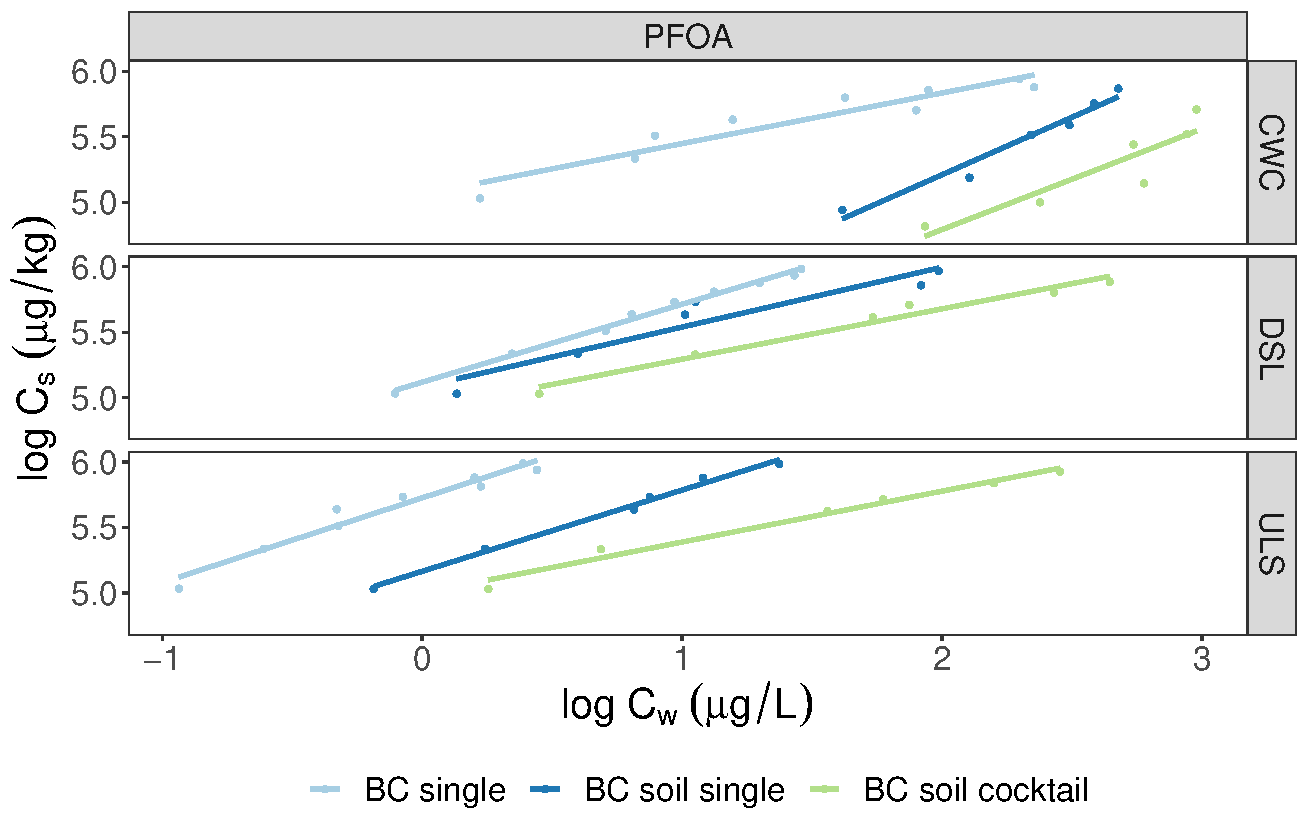
\includegraphics[width=0.8\textwidth]{R/figs/Attenuation_isotherms_PFOA.pdf}
    \caption{Sorption isotherm comparison for PFOA single-compound spike in biochar (BC single), single-compound spike in soil-biochar (BC soil single), and PFOA spiked in a cocktail in soil-biochar showing attenuation by soil and competing congeners.}
    \label{fig:PFOA_attenuation}
\end{figure}

\subsection{Freundlich sorption non-linearity}\label{sec:non-linearity}
The non-linear sorption isotherms for PFOA in \cref{fig:PFOA_nonlinear} show how sorption is attenuated at higher concentrations, and how attenuation changes in the presence of soil and soil with other PFCAs. The resulting Freundlich coefficients ($\log~K_F$ and $n_F$) for PFOA are given in \cref{tab:PFOA_Freundlich}, and the remaining compounds are in \cref{appSec:Sorption}\cref{apptab:summary_stats_all}. Two general conclusions can be drawn from these figures: 1) attenuation is higher in the presence of soil, and even higher when soil and cocktail are added together. And 2) the concentration intervals for some of the isotherms were too narrow (average $\Delta~\log~C_w$ = 1.3) to properly determine representative Freundlich coefficients for a wider concentration range. Therefore, conversion of $\log~K_F$ to either higher or lower units can be expected to be associated with greater uncertainty.

Both concentration intervals and $n_F$ should be considered together in order to predict the sorption capacity of biochars. \Cref{fig:nonlinear_OND} shows the non-linear BC-single isotherms for PFOA, PFNA and PFDA, where the degree of non-linearity is more easily visualized than the $n_F$-values alone. For example, \cref{fig:nonlinear_OND} shows that the CWC biochar isotherms have more attenuation than DSL and ULS biochars, and that $C_w$s have measurements across a wider concentration range. These findings are consistent with lower $\log~K_F$s found for CWC. \cref{fig:nonlinear_OND} also shows that the isotherms for PFNA-DSL and PFNA-ULS are nearly linear, and span aqueous concentrations only within the same order of magnitude. Higher spike concentrations, or lower BC dosages, should have been used to get isotherms that cover the regions of attenuated sorption for these biochars and compounds. What is significant is that this suggests that sludge biochars have higher sorption capacities than CWC.

The concentration range achieved for $C_w$ for the sorption isotherms was an average of 1.3 $\log$ units, in contrast to the desired concentration range over 4 $\log$ units. Poor signals were achieved for the SC1 points, and as a result were removed from the data analysis. This resulted in the spike concentration interval being reduced to two orders of magnitude (\cref{tab:spikeConcentrations}). In retrospect, spike concentrations at each $\log$ unit should have been selected instead of spreading the ten concentrations evenly across the concentration range. The CWC isotherms had the widest concentration intervals for $C_w$. This can be accounted for by the fact that CWC is the weakest sorbent of the three biochars studied.  

Electrostatic interactions between PFCAs and sediment can contribute to enhancing saturation of adsorption sites as well as intermolecular electrostatic repulsion between individual molecules \citep{higgins2006sorption,yin2022insights}. \cite{yin2022insights} presents two main explanations for why sorption of PFCAs to biochar is non-linear: 1) successive saturation of adsorption sites, and 2) the complex composition of biochar with negative, positive and neutral charges within same matrix. 

\begin{table}
\caption{Freundlich distribution coefficients and standard errors for the PFOA isotherms. Freundlich coefficients for the soil samples are the collective partition coefficients for soil and biochar because $K_d$ for soil alone was not accurate enough. All $K_F$ data are in units of $\mathrm{(\mu g/kg)/(\mu g/L)^{n_F}}$.}
\centering
\adjustbox{max width=\textwidth}{%
\begin{threeparttable}
\label{tab:PFOA_Freundlich}
\begin{tabular}{lllllll} \toprule
\multicolumn{1}{c}{Compound} & \multicolumn{1}{c}{Biochar} & \multicolumn{1}{c}{type} & \multicolumn{1}{c}{$\log~K_F$} & \multicolumn{1}{c}{$n_F$} & \multicolumn{1}{c}{$r^2$} & \multicolumn{1}{c}{$p$} \\ \midrule
PFOA & CWC & BC-S-mix  & 3.25 ± 0.48 & 0.77 ± 0.18 & 0.82 & * \\
PFOA & CWC & BC-S-sing & 3.45 ± 0.21 & 0.88 ± 0.09 & 0.96 & ** \\
PFOA & CWC & BC-sing    & 5.06 ± 0.08 & 0.39 ± 0.05 & 0.90 & *** \\
PFOA & DSL & BC-S-mix  & 4.91 ± 0.06 & 0.39 ± 0.03 & 0.97 & *** \\
PFOA & DSL & BC-S-sing & 5.08 ± 0.10 & 0.46 ± 0.08 & 0.90 & * \\
PFOA & DSL & BC-sing    & 5.12 ± 0.02 & 0.60 ± 0.02 & 0.99 & *** \\
PFOA & ULS & BC-S-mix  & 5.00 ± 0.05 & 0.39 ± 0.03 & 0.98 & *** \\
PFOA & ULS & BC-S-sing & 5.16 ± 0.03 & 0.62 ± 0.03 & 0.99 & *** \\
PFOA & ULS & BC-sing    & 5.73 ± 0.02 & 0.65 ± 0.05 & 0.95 & *** \\ \bottomrule
\end{tabular}
\begin{tablenotes}
\item Significant codes: *** $\sim$ 0.001, ** $\sim$ 0.01, * $\sim$ 0.05
\end{tablenotes}
\end{threeparttable}}
\end{table}

\begin{figure}
    \centering
    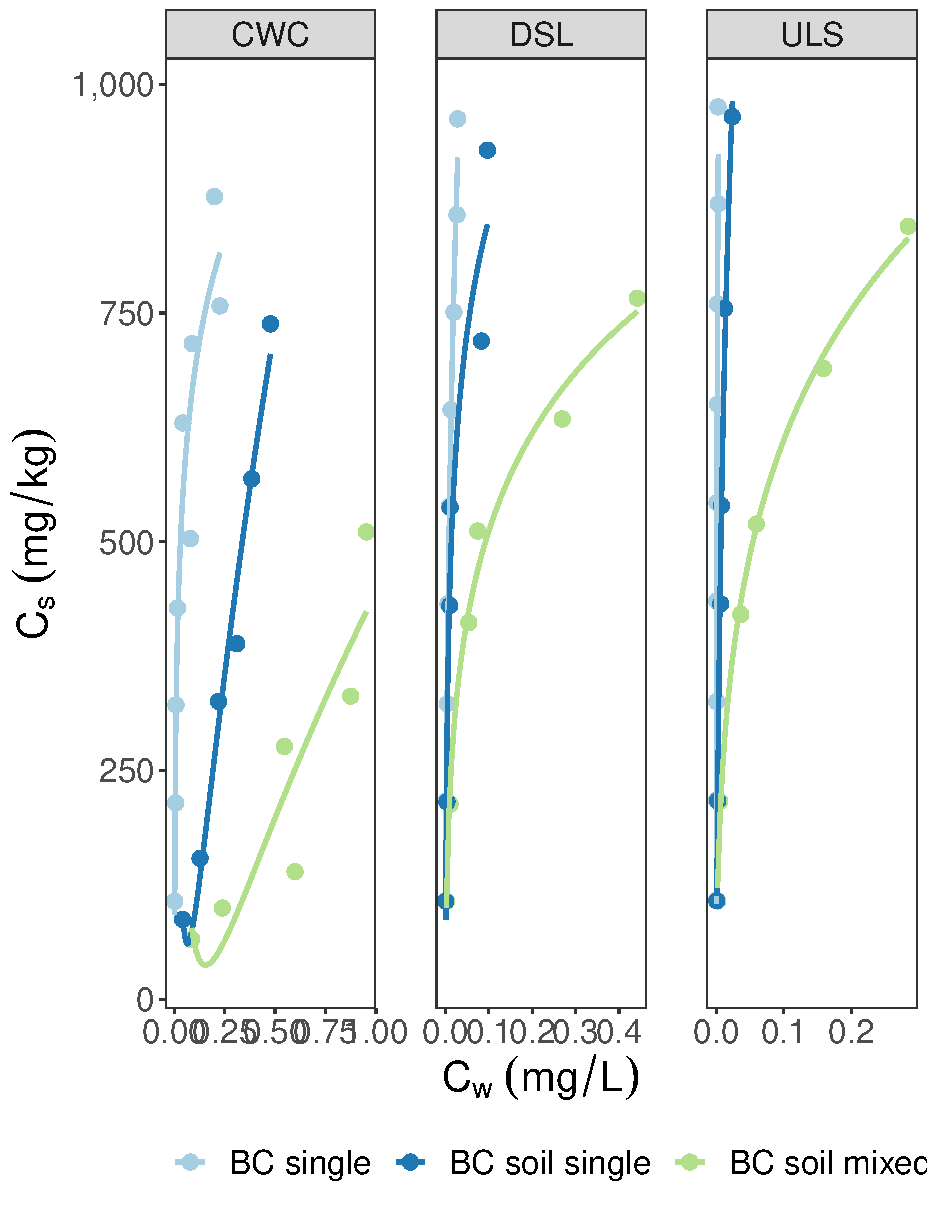
\includegraphics[width=0.8\textwidth]{R/figs/PFOA_linear.pdf}
    \caption{Non-linear sorption isotherms for PFOA in the BC-single, BC-mixed and BC-soil-mixed batch tests. Lines are fitted by a polylogarithmic function.}
    \label{fig:PFOA_nonlinear}
\end{figure}

\begin{figure}
    \centering
    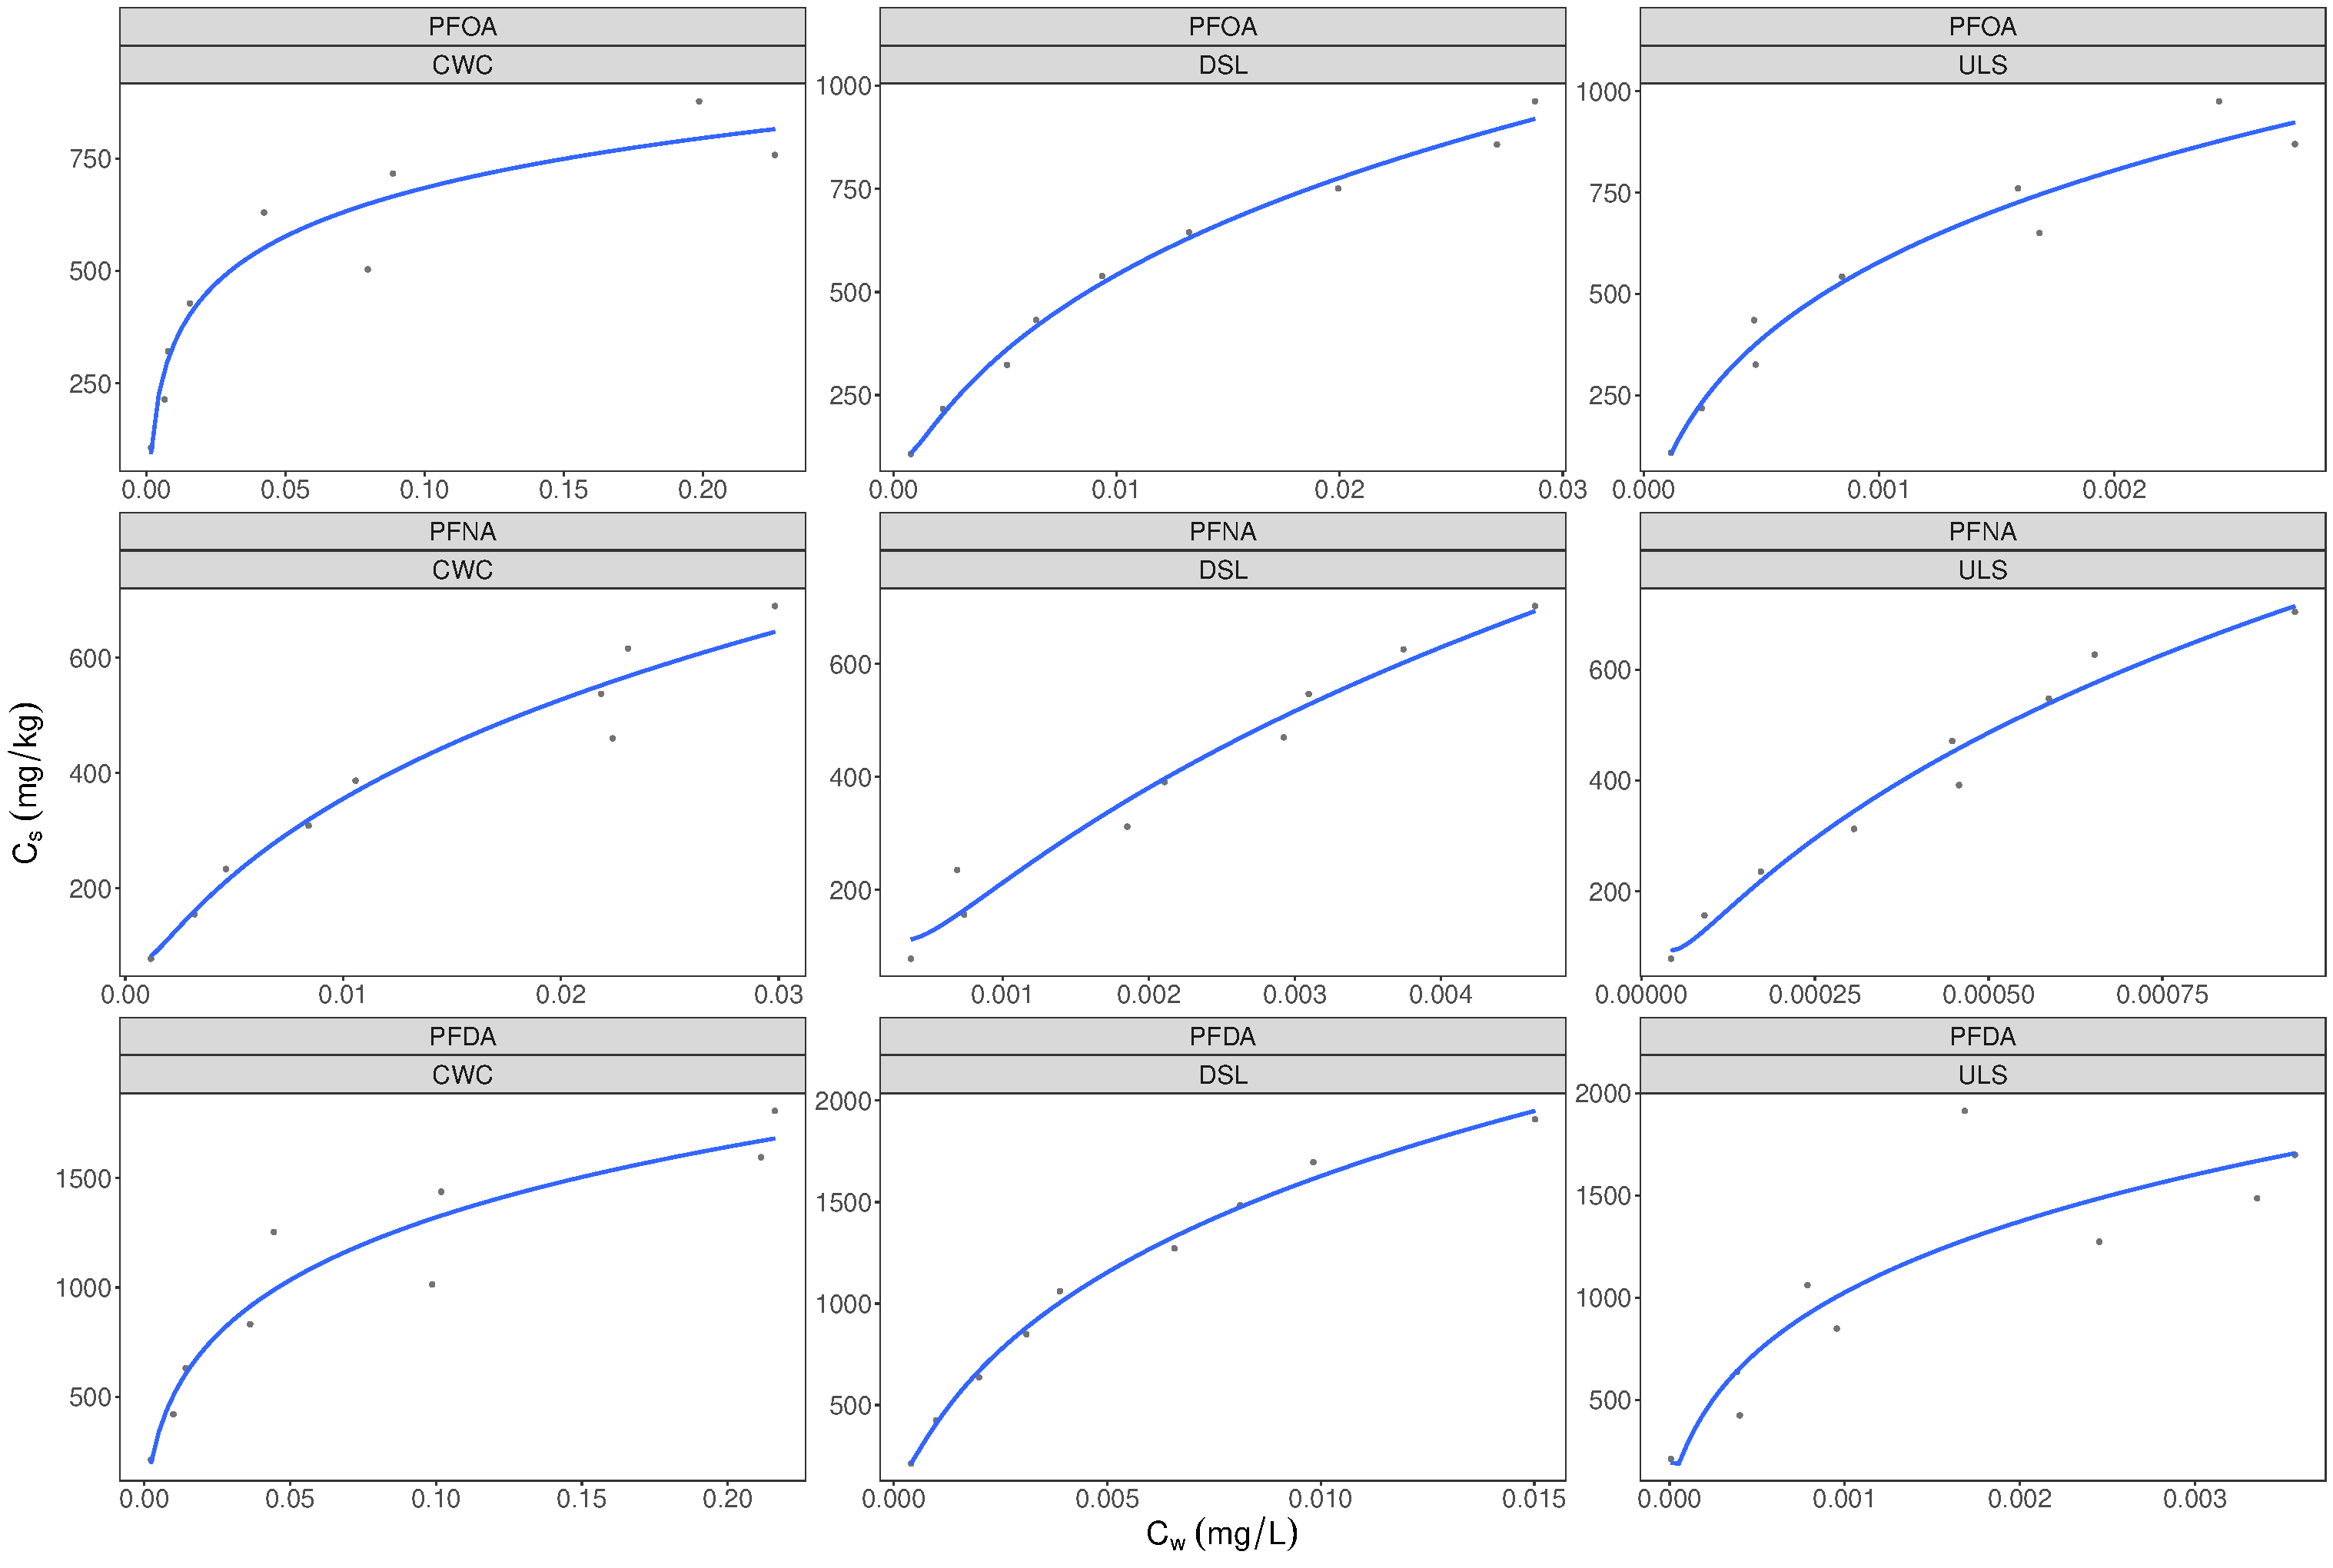
\includegraphics[width=\textwidth]{R/figs/BC_single_attenuation.pdf}
    \caption{Plots showing sorption attenuation by the presence of other PFCAs with increasing spiked concentrations. Lines are fitted by a polylogarithmic function.}
    \label{fig:nonlinear_OND} 
\end{figure}

\subsection{Attenuation by organic matter} 
Colored filtrate and humus aggregation seen during analysis of the soil batch tests indicate that sorption of organic matter (OM) to biochar is likely (see \cref{sec:S-BC}. Large humic acids (300-600 nm) clog the pores, preventing diffusion of PFAS \citep{Cornelissen2006,kluvcakova2018size}. Furthermore, the size of the organic molecules is a critical factor, as humic molecules, whose size is similar to that of PFAS, represent the greatest competition to PFAS in terms of diffusion \citep{du2014adsorption}. By the co-existence of OM and dissolved organic carbon (DOC), sorption attenuation occurs by a combination of competitive and weaker sorption of PFAS to OM and DOC, and the competitive sorption of OM to biochar. PFAS binds to OM, and it is possible that PFAS also binds to the dissolved fraction of OM (DOC). Since DOC is sorbed it is thus possible that there is sorption of DOC-PFAS complexes. Given that DOC-assisted PFAS sorption has yet not been proven, and investigating size fractionation for humic molecules was not a part of this study, the points presented here could only take place on a theoretical level.





\newpage

%Conclusions
\chapter{Implications, conclusion and recommendations for further work}\label{chap:Conclusion} \chaptermark{Conclusion}
The data generated in this research has yielded promising results for the future use of sewage sludge-based biochar (SS-BC) as a sorbent. To begin the summary of the results obtained, the initial hypotheses that represented a point of departure for the research presented, are reiterated:

\begin{enumerate}[label=\roman*]
    \item Biochar from sewage sludge is not as effective a sorbent for PFAS as biochar produced from clean wood chips due to its lower carbon-content and porosity, though it can be used as a low-cost, lower quality-class sorbent.
    \item The dominant mechanism by which PFCAs sorb to sewage sludge biochars is electrostatic attraction due to mineral-rich components. 
    \item Following from hypothesis (ii), sorption to sewage sludge biochars is not chain-length dependent and is due to electrostatic interactions by the negatively charged PFCA functional group, whereas sorption increases with chain length for clean wood chips due to predominating hydrophobic interactions with the more carbonaceous matrix of this biochar.
    \item Sorption of PFCA to biochar is attenuated by the presence of soil and other PFCAs. 
\end{enumerate}

Hypotheses (i), (ii) and (iii) were rejected. Hypothesis (i) was falsified by discovering that the SS-BCs tested in this research were \textit{better} sorbents for PFCAs than biochar from clean wood chips (CWC). $\Log~K_F$, in units of $\mathrm{(\mu g/kg)/(\mu g/L)^{n_F}}$, were in the range 5.73-6.00 for ULS biochar, 5.12-5.61 for DSL biochar, and 5.06-5.22 for CWC biochar for PFOA, PFNA, and PFDA (\cref{tab:summary_stats_single}). Despite the fact that CWC biochar had the largest surface area, the majority of its pores were too small to accommodate PFAS. The higher fraction of mesopores (2-50 nm) in the sewage sludge biochars compared to those found in clean wood chips (CWC) probably explains why the SS-BCs turned out to be such effective sorbents. Furthermore, better sorption to ULS biochar was explained by a higher carbon content (30\%) than that of DSL biochar (14\%).

Hypothesis (ii) was rejected by the observation of higher $\log~K_d$'s (at $C_w = 1 \mathrm{\mu g/L}$) with increasing perfluorinated chain length for all biochar feedstocks (\cref{fig:chainlength}). Since no apparent correlations were found between Ca or Fe-content and $\log~K_d$, electrostatic interactions are likely not the primary sorption mechanism for the SS-BCs. Since strongest sorption was measured for the biochars with higher porosity and carbon content, hydrophobic interactions is likely the dominant sorption mechanism for PFCAs to the SS-BCs. Although mechanisms responsible for the stronger sorption of ULS and DSL were proposed, these could not be fully verified due to the limited sample size of only three biochars. 

The conclusions drawn from hypothesis (ii) are directly linked to hypothesis (iii) which was also rejected for the same reasons. The poor Freundlich sorption isotherm correlations acquired for the short-chain PFCAs (PFPeA, PFHxA and PFHpA) supports the chain length-dependency of PFCAs to ULS, DSL, and CWC biochars. This relationship suggests that sorption of PFCA to SS-BCs was mainly governed by hydrophobic interactions between the C-F chain and carbonaceous aromatic surfaces. Since mineral contents were high in the strong-sorbing SS-BCs, a larger sample size is needed to understand how these influence sorption strength and mechanisms. 

Finally, hypothesis (iv) proved to be correct. Attenuation factors (AFs) ranged from 3-10 for PFOA in the presence of soil, 6-140 for PFOA, PFNA, and PFDA in a mixture of PFCAs, and 8-138 for PFOA, PFNA, and PFDA in the presence of soil and other PFCAs (\cref{tab:attenuation}). Despite large variations in AFs, the presence of other PFCAs was responsible for a stronger degree of attenuation than the presence of soil. The presence of soil in the PFCA-mixture increased attenuation by an additional 27\%. This suggests that the sorbents could be more effective for filtration in waste water treatment than in soil remediation, and especially in moderately contaminated wastewater. 

%%%%%%%%%%%%%%%%%%%%%%%%%%%%%%%%%%%%%%%%%%%%%%%%%%%%%%%%%%%%%%%%%%%%%%%%%%%%%%%%%%%%%
%%%%%%%%%%%%%%%%%%%%%%%%%%%%%%%%%%%%%%%%%%%%%%%%%%%%%%%%%%%%%%%%%%%%%%%%%%%%%%%%%%%%%
\section{Application of sewage sludge biochar in the treatment of wastewater \label{sec:application}}
The results from this study demonstrate that the ULS and DSL biochars bind PFCA strongly at concentrations that are many times higher than most environmental concentrations. The SS-BCs tested have shown to sorb equally strongly, or stronger than, several activated carbons (AC) reported in previous literature \citep{Kupryianchyk2016b, hansen2010sorption, silvani2019can}. Therefore, some rough estimates have been made for how effective the ULS and DSL biochars are for removing PFAS from wastewater in Norway. 

Based on samples obtained by a Norwegian survey conducted in late 2020 (Gabriela Castro Varela, NTNU, unpublished data), Norwegian wastewater treatment plant influents contain between 0.1-1 $\mathrm{\mu g/L}$. The Freundlich distribution coefficients derived for the ULS and DSL biochars from the BC-soil-mix sorption isotherms can be used to estimate the sorption efficiency of the biochars for Norwegian wastewater. The BC-soil-mix isotherms were chosen because one can assume attenuation when they are used in treating wastewater. Removal efficiency of PFOA was used for simplicity. This estimate assumes no kinetic limitations during the wastewater treatment procedure, equilibrium conditions, and a water/BC ratio of 500. Linear sorption ($n_F = 1)$ can be assumed for the application of unused SS-BC to Norwegian wastewater because the wastewater concentration was two orders of magnitude below the lowest spiked concentration for the isotherms. Thus, $\log~K_F$ = $\log~K_d$ = 5.00 and 4.91 for ULS and DSL biochars respectively. To be conservative, these calculations were based on a PFOA wastewater concentration of $1 \mathrm{\mu g/L}$. These values result in the potential reduction of PFOA from wastewater by 99.5 and 99.4\%, that is, equilibrium aqueous concentrations of 0.005 and 0.006 $\mathrm{\mu g/L}$ by the ULS and DSL biochars. Clearly, these SS-BCs have the potential to be effective in removing PFAS from Norwegian wastewater. 

Equilibrium aqueous concentrations measured at higher concentrations say something about the sorption capacities of the ULS and DSL biochars, and can therefore give an indication of how long carbon filters used for wastewater treatment can be expected to reduce PFAS concentration to an acceptable level. As is widely accepted, and supported by the findings of this thesis, sorption to biochar is weaker (attenuated) at higher contaminant concentrations. Due to the kinetic aspects of the sorption process, the following assessment is only \textit{indicative} of filtration capacity as there are differences between a batch test with a spiked concentration, and the steady flow of a lower concentration. Using the same assumptions underlying the previous example, but now with an initial PFOA concentration of 1.9 mg/L in a total PFCA cocktail concentration of 10 mg/L, 85.5 and 77.7\% would be retained by ULS and DSL respectively, versus $>$99\% at 1 $\mathrm{\mu g/L}$. The sorption capacity of ULS and DSL biochars at this point would result in equilibrium aqueous PFOA concentrations of 0.28 and 0.44 mg/L---post-treatment levels that would be unacceptable. Hence, the filter would need to be exchanged before this point. Tests that account for wastewater residence time, flow rate, bed volumes, and sorbent dose, are factors that would need to be considered in order to design a water purification solution that uses SS-BCs, and is beyond the scope of the present study. 

\subsection{Considerations for commercializing sludge chars as sorbents}
The sorption strength of sewage sludge biochars was tested in a controlled laboratory environment, with low-TOC soil, and artificially spiked PFCAs. The results from this research do not, therefore, take into account the heterogeneity of sewage sludges, variations in the organic matter contents of soils that the sorbents will potentially be applied to, and the potential competition for sorption sites from a range of other possible contaminants in soil and water in need of remediation. All of the variables mentioned above will influence the sorption strength of SS-BCs. 

Since the results from this study showed poor sorption affinity to PFPeA, PFHxA, and PFHpA, consideration should also be given to ensure that short-chain PFASs do not slip through wastewater treatment systems that use SS-BC. For this reason, Lindum considers the application of SS-BCs more as a pre-treatment sorbent, to be followed by treatment using a stronger sorbent that is more effective in retaining short-chain PFAS. Also important to consider is the potential risk of residual contaminants in biochars produced from contaminated feedstocks. 

%The Danish limit for 2 ng/L PFOA, PFOA, PFNA, and PFHxS for safe drinking water has not been reached \citep{Danmark2021grenseverdier}, appendix 1 d. 2 ng/L is considered safe levels for drinking water. Attention could also be given to investigating the relationship between soil organic carbon and the biochar dosage required to reduce PFAS pore water concentrations down to the environmental quality standards in soils determined by Norwegian Environment Agency (2020) which are 0-9.1μg/L PFOA for class II/good. 
%\citep{PFOS2018grenser}: Norwegian Water Framework Directive: PFOS in surface water limit 36 $\mathrm{\mu g/L}$. 

\section{Revenue estimates for commercial production of sewage sludge biochar}
The following is a case example that gives a rough idea of the revenue potential of a scenario in which 100 \% of the activated carbon used for wastewater treatment is replaced with SS-BC. The Norwegian WWTP, VEAS, purchases 2 tonnes of AC annually for wastewater treatment. Market prices for AC range from 600 - 1,000 \texteuro/tonne. For VEAS, replacing AC with SS-BC would result in annual savings from 200 - 1,000 \texteuro, equivalent to a cost reduction of 17-50\%. This assumes that SS-BC has a starting price of 500 \texteuro/tonne. How many WWTPs are there in Norway?

A second case presents a prime example of a circular economy scenario. Wastewater from Ullensaker WWTP, the project partner that provided the ULS sludge analyzed in this thesis, contains 3.8 $\mathrm{\mu g/L}$ (Varela, unpublished). This is the highest level of PFAS concentration found among the six Norwegian WWTPs monitored. High concentrations of PFAS at the Ullensaker WWTP have been attributed to the use of aqueous film forming foam at a nearby firefighting training facility \citep{Hale2017fire}. In this scenario, Ullensaker WWTP adapts pyrolysis technology that can produce biochar from the high PFAS-level wastewater they are paid to remediate. The resulting ULS biochar is applied directly as a PFAS sorbent to wastewater. With an influent total PFAS concentration of 3.8 $\mathrm{\mu g/L}$ in Ullensaker wastewater, linear sorption can be assumed. Based on the BC-S-mix isotherm used in this study, $\log~K_ds$ for ULS biochar are 5.00, 5.22, and 5.62 for PFOA, PFNA, and PFDA. reduces water concentrations to $<$20 ng/L ($>$99.5\%). Applying this solution at the Ullensaker WWTP site would mean eliminating transportation-related costs. In addition, SS-BCs have low production costs that are estimated to be 100 \texteuro/tonne. If SS-BCs can be produced for 100\texteuro/tonne, and sold for 500 \texteuro/tonne, the revenue from pyrolyzing all sewage sludge in Norway would be 3,600,000 \texteuro/year = 36 million NOK annually. 

In summary, there appear to be several benefits associated with replacing AC with SS-BC: 1) PFAS present in wastewater can, for all intents and purposes, be eliminated by pyrolysis. Preliminary data from one of the partners in this study shows reductions from 90-95\% (Erlend S{\o}rmo unpublished), 2) biochar that previously contained PFAS can now be applied to sorb even more PFAS-contaminated sludge right at the production site, 3) reduced annual expenses for the purchase of currently available commercial sorbents, and 4) WWTPs can increase their profitability and at the same time contribute to carbon sequestration. A rough calculation of the carbon sequestration potential of SS-BCs has been made and is presented in the following section. 

\section{Carbon sequestration potential}
Since a commercial trade in carbon credits has opened up, the potential sale of SS-BCs at a global scale could be highly attractive. Assuming that SS-BC replaces the entire annual demands for AC in Norway and Europe, it is possible to make a rough estimate of the carbon sequestration potential of SS-BCs. Carbon dioxide equivalents (\acrshort{CO2eq}) can be calculated, where one $\mathrm{CO_2-eq}$ is the equivalent of one tonne of sequestered $\mathrm{CO_2}$. Annual demands for AC in Norway are approximately 1,700 tonnes/year, and 165,000 tonnes/year for Europe as a whole \citep{schmidt2019pyrogenic}. On average, sewage sludge biochars contain 20\% carbon (C), of which 70-80 \% is assumed to be stable over time \citep{schmidt2019pyrogenic}. This is equivalent to 1,000 and 100,000 annual CO\textsubscript{2}-eq for Norway and Europe respectively. Considering the current EU CO\textsubscript{2} trading price of 90 \texteuro/CO\textsubscript{2}-eq, this translates into annual carbon credit values of 90,000 and 8,800,000 \texteuro. 

For the production of the 1,700 tonnes of SS-BC needed annually to replace AC, assuming 30\% yield, a mere 7\% of the 200,000 tonnes w.w. (30,000 d.w.) of sewage sludge generated in Norway each year would be needed. This fraction could be much higher if soil remediation can also be done with SS-BC as well as the application of SS-BC as fertilizers in agriculture. However, much more research is needed before this point can be reached. Despite a wide range of both technical and legislative challenges, a great deal of research is being done to corroborate initial research that suggests that nearly all microplastics, heavy metals, and organic pollutants, including PFAS, are either combusted or immobilized at high pyrolysis temperatures (S\o rmo, unpublished). In a best-case-scenario, the 93\% of sewage sludge remaining after sorbent production could still be pyrolyzed into BC, and used, for example, in place of bio-based fertilizers in agriculture. \textit{Raw} biosolids contain microplastics, heavy metals, and various organic pollutants. These same masses can potentially safely be applied to agricultural fields \textit{after} pyrolysis. In addition, though further research is needed, pyrolyzed sludge could prove to increase soil fertility more effectively than non-pyrolyzed biosolids. Not only would this represent increased carbon sequestration, but it would serve as an additional incentive for SS-BC manufacturers to maximize their biochar yields from raw sewage sludge, thereby creating products that are attractive on the voluntary carbon credit market. 

It is tempting to further speculate on the revenues a company like Lindum AS could expect by processing all sewage sludge using pyrolysis. They currently generate revenues by 1) treating sewage sludge, and 2) using some of the fractions to produce bio-gas. Managing to utilize the final fraction, digestate, could further increase the company's revenues per tonne of processed raw sewage sludge. SS-BC production costs of 100 \texteuro/tonne will likely represent a tiny fraction of the total revenue that can be expected from each tonne of raw sewage sludge received. 

%%%%%%%%%%%%%%%%%%%%%%%%%%%%%%%%%%%%%%%%%%%%%%%%%%%%%%%%%%%%%%%%%%%%%%%%%%%%%%%%%%%%%
%%%%%%%%%%%%%%%%%%%%%%%%%%%%%%%%%%%%%%%%%%%%%%%%%%%%%%%%%%%%%%%%%%%%%%%%%%%%%%%%%%%%%

\section{Waste-based biochar for sustainable development \label{sec:SDGs}}
Within Norway and the EU, a number of research initiatives have been taken to study possible applications of waste-based biochar sorbents that could contribute to achieving the following   2030 United Nations Sustainable Development Goals (\acrshort{SDGs}) \citep{SDGs2015}:
\begin{itemize}
    \item \textbf{SDG 6}:  Clean water and sanitation
    \item \textbf{SDG 9}:  Industry, innovation and infrastructure
    \item \textbf{SDG 11}: Sustainable cities and communities
    \item \textbf{SDG 12}: Responsible consumption and production
    \item \textbf{SDG 13}: Climate action
    \item \textbf{SDG 14}: Life below water
    \item \textbf{SDG 15}: Life on land
\end{itemize}

and the European Green Deal of 2020. The European Green Deal of July 14, 2021 lists development of biochar as one of the most important economic means to achieve the goal of making Europe the first climate-neutral continent in the world. The 4 per mille initiative, Soils for Food Security and Climate, was launched by France during the UN climate change conference in December, 2015 (COP21). The 4 per 1000 mission is to increase soil carbon stocks in the first 30-40 cm of soil by 4 \textperthousand  annually as a means of complementing what is necessary efforts to compensate for global fossil-based GHG emissions. The goal is to scale biochar for global agricultural and remediation markets. If applied correctly, biochar can play an important role in sequestering carbon, and at the same time serve as a soil amendment and fertilizer in agriculture. However, this must be done carefully because application of biochar in soil has been shown to have a priming effect on soil-native C by improving microbial populations, thereby influencing the decomposition rate of organic matter \citep{Ahmad2014}. In most cases however, negative priming is seen, and biochar actually helps to increase natural organic matter content in soils \citep{chen2019competitive,weng2018accumulation}. The International Biochar Initiative (IBI) is a collaborative platform for science, industry, agriculture, government, and non-governmental organizations, such as the European Biochar Certificate (EBC) which creates awareness about the benefits of biochar, and develops biochar standards for safe and sustainable use. 

\section{Final recommendations}
This thesis has proposed a set of mechanisms that are expected to explain the differences in sorption of PFCAs to biochar derived from raw sewage sludge, digested sludge, and clean wood chips. It has indicated the significant potential of biochar in a circular economy, and its application as a sorbent for wastewater treatment, or as an amendment to PFAS-contaminated soil. This study is one of the first to show that biochar made from two different sewage sludge substrates can be used to reduce PFAS concentrations in water by 88 $\pm$ 22\% at a dosage of only 0.1 g. These results and their analysis also raise new research questions within the relatively recent research area of PFAS-sorption to sewage sludge biochars. Conducting multivariate regression analyses between PFAS sorption strenght and factors such as surface area, pore volume, carbon content, and mineral contents (mainly Ca and Fe) will be necessary to confirm the sorption mechanisms proposed in this work, and to draw more definitive conclusions than those presented here.  In addition to studying the effect of activation of sludge chars on sorption strength, additional research could also determine capacity tests for sewage sludge-based biochar filters, sorption strength to other PFAS groups, especially PFSA, competition with PAHs, and other contaminants that are commonly present in wastewater. Attention could also be given to investigating the relationship between soil organic carbon, and the biochar dosage required to reduce PFAS pore water concentrations to an acceptable level. 

Increased potential for carbon sequestration, and increased commercial valorization of sewage sludge, are highly promising for the incorporation, and ultimately, the replacement of existing fossil-derived sorbents with sewage-sludge based sorbents. Should further studies corroborate the findings presented in this study, the commercial and environmental benefits would be nothing less than sensational. 








\newpage

%Further work
\chapter{Recommendations for further work}\label{chap:furtherwork}


%\newpage

%Quality controls notes:

Sample matrix refers to everything present in the sample except for the target analytes. 

Reagent blank contains no sample matrix and no analytes, only labeled IS to check contamination during the extraction protocol. The reagent blank is brought through the entire extraction protocol and analyzed in the same manner as the test samples. Contamination from test tubes, reagents or other introductions of contamination will show up on the instrument results from this quality control sample. If contaminated we know that it comes from the protocol and needs to be subtracted from the rest of the samples.  % midlertidig for å se hvordan det blir. Flyttet til litterature
%\input{Konklusjon}
%input{Referanser}
% Symbolliste
%\include{Chapters/Symbolliste}
%\include{Chapters/Refferanser}
%\newpage

\bibliography{Kilder/Biochar-PFAS,Kilder/Rapporter,Kilder/History,Kilder/Jord-PFAS,Kilder/PFAS}
\addcontentsline{toc}{chapter}{Bibliography}

%\end{comment}
%%%%%%%%%%%%%%%%%%%%%%%%%%%%%%%%%%%%%%%%%%%%%%%%%%%%%%%%%%%%%%%%%%%%%%%%%%%%%%%%%%%%%%%%%%%%%%%%%%%%%%%%%%%%%%%%%%%%%%%%%%%%%%%%%%%%%%%%%%%%%%%%%%%%%%%%%%%%%%%%%%%%%%%%%%%%%%%%%%%%%%%%%%%%%%%%%%%%%%
\clearpage % for ikke ha romertall på siste side av references

%Glossary
\pagenumbering{roman}%romertall
\setcounter{page}{18}%starter sidetall på rett side, denne må oppdateres ved endelig dokument



%\addcontentsline{toc}{chapter}{Glossary}
%\input{Lister/Glossary}

% Formatering av appendix liste
%\clearpage %Brukt i artikkel
%\titleformat{\chapter}[block]{\Huge\bfseries}{Appendix \thechapter}{1em}{}
\setcounter{secnumdepth}{0}

%%  APPENDIX aka vedlegg
% Fjerner appendix figurer & tabeller fra lister https://tex.stackexchange.com/questions/213523/remove-appendix-tables-and-figures-from-list-of-figure-tables
\let\svaddcontentsline\addcontentsline
\renewcommand\addcontentsline[3]{%
  \ifthenelse{\equal{#1}{lof}}{}%
  {\ifthenelse{\equal{#1}{lot}}{}{\svaddcontentsline{#1}{#2}{#3}}}}
\appendix

% Formatering for resten av appendix
\setcounter{equation}{0}        % starter formler på 0
\setcounter{secnumdepth}{2}     % A.1, A.2 etc

\titleformat{\section}          % Kun på sections
{\normalfont\bfseries\centering} % Bold sentrert
{\thesection}                   % nummererer (A.1, A.2 etc.)
{0.5em}                         % Avstand mellom label    (nummerering) og tekst i section-tittel
{}  %https://www.overleaf.com/learn/latex/sections_and_chapters

\setlength{\headsep}{0.3cm} % avstand topptekstlinje til tekst for å få plass til mer av pdf: scale 0,85, evt justere for andre PDF størrelser

\addtocontents{toc}{\protect\setcounter{tocdepth}{0}}

% \ref{appSec:"vedleggslabel"}       gir: A,B,C...
% \ref{app:"PDFlabel"}               gir: A1, A2, B1, B2 etc.
% Merk at her brukes ikke \cref som i resten av dokumentet 

% label for hver pdf plasseres i pagecommanden etter "\section{}"
% Eks.: ..., pagecommand={\subsection{Min subsection}\label{app:OedoILs01LOG}},...

\chapter*{Appendices} % Overskrift (start på vedlegg) suppresser kapitteltall
    \phantomsection % For hyperref til funke når suppressed kapitteltall
    \addcontentsline{toc}{part}{Appendices}%
    \markboth{Appendices}{Appendices}% https://latex.org/forum/viewtopic.php?t=1309
List of appendices % Oppdater siste tall (XYZ) til siste vedleggsnummer for hvert vedlegg
\begin{itemize}
    \item \cref{appSec:ETIA}.number--number: \nameref{appSec:ETIA}
    \item \cref{appSec:IsothermSetup}. number--number: \nameref{appSec:IsothermSetup}
    \item \cref{appSec:LCMS}. number--number: \nameref{appSec:LCMS}
    \item \cref{appSec:misclab}. number--number: \nameref{appSec:misclab}
    \item \cref{appSec:elements}. number--number: \nameref{appSec:elements}
    \item \cref{appSec:pollution}. number--number: \nameref{appSec:pollution}
\end{itemize}

% Ta inn vedlegg i ønsket rekkefølge og oppdater evt listen ovenfor
\chapter{Images from ETIA unit}\label{appSec:ETIA} 

In the following section are images from the ETIA pyrolysis system at Lindum waste handling company (Drammen, Norway) presented. 


\begin{figure}
    \centering
    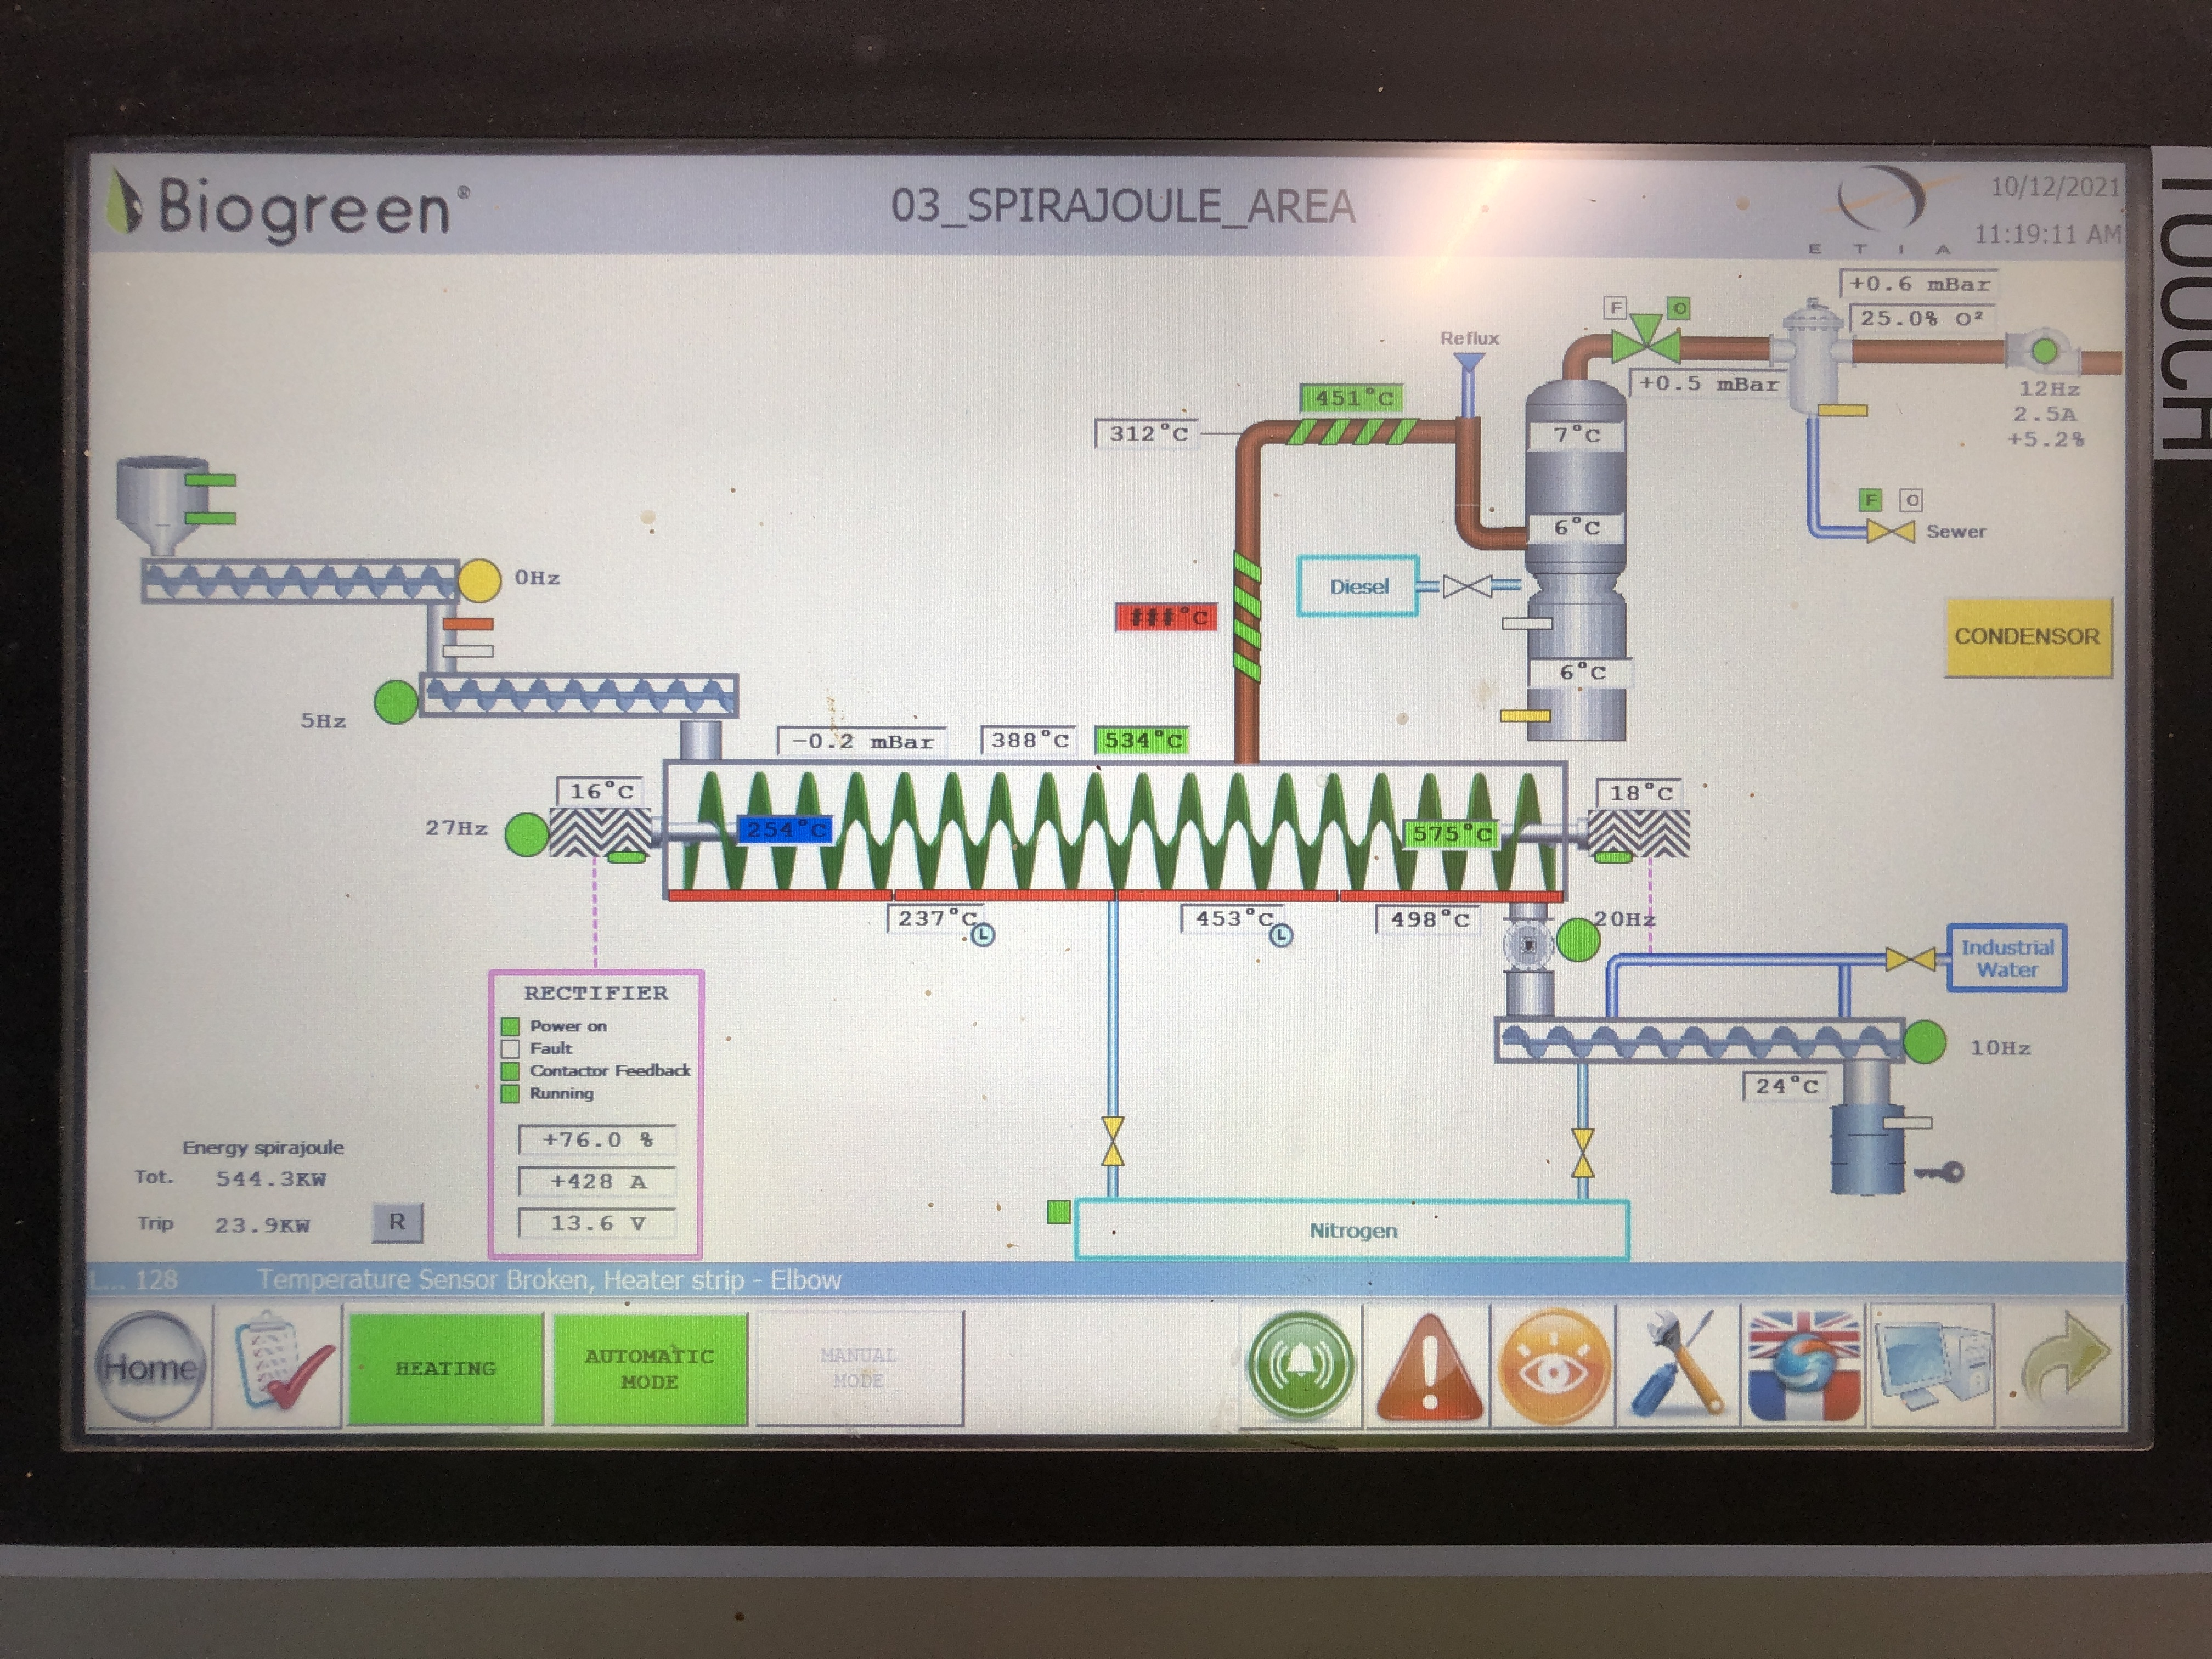
\includegraphics[width=0.7\linewidth,scale=0.7]{Bilder/Pyrolysis/Screen.png}
    \caption{Screen that displays monitoring of temperatures along the pyrolysis system developed by Biogreen\textsuperscript{\textregistered}.}
    \label{appFig:screen}
\end{figure}
\chapter{Sorption isotherm setup}\label{appSec:IsothermSetup}
In the following section, raw data for PFCA standard concentration calculations, mass of biochar weighed for each batch test, and pipetting volume are presented.

\begin{table}[h]
\centering
\caption{Concentration of first PFCA standard solution in 10 mL volumetric flasks accounted for purity of the PFCAs produced by Merck.}
\label{appTab:purityMass}
\begin{tabular}{lllll}
\toprule
Compound & Mass PFCA (g) & Purity (\%) & Mass PFCA (g) & {[}PFCA{]} (g/L) \\ 
& weighed & & accounted for purity & in   10 mL MeOH \\ \midrule
PFPeA & 0.0666 & 97 & 0.0646 & 6.46 \\
PFHxA & 0.0244 & 97 & 0.0237 & 2.37 \\
PFHpA & 0.0560 & 99 & 0.0554 & 5.54 \\
PFOA & 0.0116 & 95 & 0.0110 & 1.10 \\
PFNA & 0.0153 & 97 & 0.0148 & 1.48 \\
PFDA & 0.0114 & 98 & 0.0112 & 1.12 \\ \bottomrule
\end{tabular}
\end{table}

\begin{table}
\centering
\caption{Expected concentration of PFCA standards based on weight of native PFCA and dilution calculations versus analytical concentration by LC-MS/MS.}
\label{appTab:expConc}
\adjustbox{max width=\textwidth}{%
\begin{tabular}{lrrrrr} \toprule
 & \multicolumn{1}{l}{Me-OH standard (g L\textsuperscript{-1})} & \multicolumn{1}{l}{C11 (\textmu g L\textsuperscript{-1})} & \multicolumn{1}{l}{C12 (\textmu g L\textsuperscript{-1})} & \multicolumn{1}{l}{C13 (\textmu g L\textsuperscript{-1})} & \multicolumn{1}{l}{Analytical conc. (\textmu g L\textsuperscript{-1}}\\ \midrule
PFPeA & 6.46 & 5 168 & 103 & 15.5 & \\
PFHxA & 2.37 & 14 201 & 284 & 20.7 & \\
PFHpA & 5.60 & 3 360 & 27 & 10.2 & \\
PFOA & 1.16 & 13 920 & 557 & 13.4 & \\
PFNA & 1.53 & 18 360 & 367 & 10.0 & \\
PFDA & 1.14 & 17 100 & 684 & 10.3 & \\ \bottomrule
\end{tabular}}
\end{table}

\begin{table}
\centering
\caption{Mass biochar from Clean Wood Chips (CWC) weighed for each sample (n=60) (0.1000 $\pm$ 0.0004 g, \textmu = 0.1006 g, CV = 0.4 $\%$) C1-10 refers to the ten spike-concentrations for each PFCA batch test.}
\label{appTab:CWCmass}
\adjustbox{max width=\textwidth}{%
\begin{tabular}{lllllllllll}
\toprule
 & \multicolumn{10}{c}{Mass (g)} \\ \cline{2-11}
Compound & C1 & C2 & C3 & C4 & C5 & C6 & C7 & C8 & C9 & C10 \\ \midrule
PFPeA & 0.1008 & 0.1007 & 0.1007 & 0.1009 & 0.1014 & 0.1013 & 0.1011 & 0.1004 & 0.1009 & 0.1004 \\
PFHxA & 0.1014 & 0.1007 & 0.1014 & 0.1006 & 0.1002 & 0.1004 & 0.1014 & 0.1007 & 0.1004 & 0.1000 \\
PFHpA & 0.1005 & 0.1010 & 0.1005 & 0.1004 & 0.1009 & 0.1005 & 0.1002 & 0.1006 & 0.1007 & 0.1006 \\
PFOA & 0.1007 & 0.1008 & 0.1005 & 0.1009 & 0.1009 & 0.1002 & 0.1005 & 0.1006 & 0.1006 & 0.1009 \\
PFNA & 0.1002 & 0.1005 & 0.1004 & 0.1008 & 0.1008 & 0.1003 & 0.1002 & 0.1006 & 0.1006 & 0.1002 \\
PFDA & 0.1003 & 0.1001 & 0.1001 & 0.1001 & 0.1001 & 0.1003 & 0.1000 & 0.1005 & 0.1007 & 0.1007 \\ \bottomrule
\end{tabular}}
\end{table}


\begin{table}
\centering
\caption{Mass biochar from Ullensaker Sludge (ULS) weighed for each sample (n=60) (0.1000 $\pm$ 0.0003 g, \textmu = 0.1004 g, CV = 0.3 $\%$) C1-10 refers to the ten spike-concentrations for each PFCA batch test.}
\label{appTab:ULSmass}
\adjustbox{max width=\textwidth}{%
\begin{tabular}{lllllllllll}
\toprule
 & \multicolumn{10}{c}{Mass (g)} \\ \cline{2-11}
Compound & C1 & C2 & C3 & C4 & C5 & C6 & C7 & C8 & C9 & C10 \\ \midrule
PFPeA & 0.1007 & 0.1003 & 0.1004 & 0.1009 & 0.1009 & 0.1004 & 0.1009 & 0.1003 & 0.1000 & 0.1002 \\
PFHxA & 0.1009 & 0.1009 & 0.1003 & 0.1010 & 0.1002 & 0.1001 & 0.1006 & 0.1001 & 0.1000 & 0.1005 \\
PFHpA & 0.1001 & 0.1005 & 0.1004 & 0.1000 & 0.1004 & 0.1003 & 0.1005 & 0.1009 & 0.1005 & 0.1004 \\
PFOA & 0.1007 & 0.1000 & 0.1001 & 0.1009 & 0.1000 & 0.1001 & 0.1005 & 0.1001 & 0.1000 & 0.1002 \\
PFNA & 0.1001 & 0.1000 & 0.1000 & 0.1006 & 0.1000 & 0.1006 & 0.1005 & 0.1007 & 0.1007 & 0.1006 \\
PFDA & 0.1005 & 0.1005 & 0.1001 & 0.1008 & 0.1005 & 0.1001 & 0.1004 & 0.1002 & 0.1000 & 0.1003 \\ \bottomrule
\end{tabular}}
\end{table}

\begin{table}
\centering
\caption{Mass biochar from Biorest Lindum (BRL) weighed for each sample (n=60) (0.1000 $\pm$ 0.0003 g, \textmu = 0.1005 g, CV = 0.3 $\%$) C1-10 refers to the ten spike-concentrations for each PFCA batch test.}
\label{appTab:BRLmass}
\adjustbox{max width=\textwidth}{%
\begin{tabular}{lllllllllll}
\toprule
 & \multicolumn{10}{c}{Mass (g)} \\ \cline{2-11}
Compound & C1 & C2 & C3 & C4 & C5 & C6 & C7 & C8 & C9 & C10 \\ \midrule
PFPeA & 0.1003 & 0.1006 & 0.1000 & 0.1005 & 0.1007 & 0.1009 & 0.1005 & 0.1006 & 0.1007 & 0.1007 \\
PFHxA & 0.1003 & 0.1008 & 0.1004 & 0.0999 & 0.1004 & 0.1001 & 0.1002 & 0.1002 & 0.1007 & 0.1004 \\
PFHpA & 0.1005 & 0.1009 & 0.1010 & 0.1000 & 0.1006 & 0.1007 & 0.1007 & 0.1003 & 0.1005 & 0.1004 \\
PFOA & 0.1006 & 0.1008 & 0.1009 & 0.1002 & 0.1004 & 0.1002 & 0.1006 & 0.1001 & 0.1001 & 0.1000 \\
PFNA & 0.1010 & 0.1009 & 0.1010 & 0.1003 & 0.1002 & 0.0999 & 0.1005 & 0.1010 & 0.1005 & 0.1008 \\
PFDA & 0.1001 & 0.1007 & 0.1003 & 0.1010 & 0.1006 & 0.1008 & 0.1008 & 0.1001 & 0.1010 & 0.1004 \\ \bottomrule
\end{tabular}}
\end{table}

\begin{table}
\centering
\caption{Volume pipetted from working standards using different combinations of micro- (5-50 {\textmu}l and 200-1000 {\textmu}l) and milli pipettes (2-10 mL).}
\label{appTab:pipetting}
\adjustbox{max width=\textwidth}{%
\begin{tabular}{lrrrrrrrrrr} \toprule
\multicolumn{1}{c}{\textbf{}} & \multicolumn{10}{c}{Pipetting   volume (mL) from C11 (white) and C12 (grey)} \\ \cline{2-11} 
Compound & V1 & V2 & V3 & V4 & V5 & V6 & V7 & V8 & V9 & V10 \\ \midrule
PFPeA & \cellcolor[HTML]{C0C0C0}0.0145 & 0.314 & 0.653 & 0.967 & 1.305 & 1.620 & 1.935 & 2.274 & 2.900 & 2.902 \\
PFHxA & \cellcolor[HTML]{C0C0C0}0.0105 & 0.238 & 0.467 & 0.705 & 0.933 & 1.180 & 1.408 & 1.637 & 1.866 & 2.113 \\
PFHpA & \cellcolor[HTML]{C0C0C0}0.0240 & \cellcolor[HTML]{C0C0C0}23.250 & 0.410 & 0.632 & 0.855 & 1.079 & 1.302 & 1.525 & 1.749 & 1.935 \\
PFOA & \cellcolor[HTML]{C0C0C0}0.0110 & 0.475 & 0.960 & 1.437 & 1.922 & 2.398 & 2.874 & 3.360 & 3.843 & 4.310 \\
PFNA & \cellcolor[HTML]{C0C0C0}0.0220 & 0.483 & 0.967 & 1.457 & 1.935 & 2.425 & 2.915 & 3.390 & 3.880 & 4.357 \\
PFDA & \cellcolor[HTML]{C0C0C0}0.0365 & 1.623 & 3.245 & 4.868 & 6.490 & 8.115 & 9.737 & 11.360 & 12.982 & 14.620 \\ \bottomrule
\end{tabular}}
\end{table}

\begin{table}
\centering
\caption{Mass for each PFCA batch test prepared in 50 mL PP Falcon tubes, assuming a density of water of 1 g/mL (50.0000 $\pm$ 0.02 mL, \textmu = 50.0075 mL, CV=0.04$\%$).}
\label{appTab:milliQ}
\adjustbox{max width=\textwidth}{%
\begin{tabular}{lllllllllll} \toprule
 & \multicolumn{10}{c}{Mass (g) water weighed} \\ \cline{2-11}
Compound & V1 & V2 & V3 & V4 & V5 & V6 & V7 & V8 & V9 & V10 \\ \midrule
PFPeA & 50.0129 & 50.0108 & 50.0016 & 50.0020 & 49.9934 & 50.0001 & 50.0072 & 49.9916 & 49.9902 & 49.9943 \\
PFHxA & 50.0059 & 50.0262 & 49.9934 & 50.0107 & 50.0093 & 49.9938 & 49.9971 & 50.0015 & 50.0062 & 50.0001 \\
PFHpA & 50.0123 & 50.0084 & 50.0005 & 50.1474 & 49.9976 & 50.0055 & 49.9948 & 50.0037 & 50.0165 & 49.9950 \\
PFOA & 50.0095 & 50.0092 & 50.0128 & 49.9976 & 50.0055 & 50.0053 & 50.0036 & 50.0143 & 50.0090 & 49.9940 \\
PFNA & 50.0149 & 50.0030 & 49.9966 & 50.0463 & 50.0070 & 49.9856 & 50.0024 & 50.0062 & 50.0161 & 50.0445 \\
PFDA & 50.0120 & 50.0021 & 50.0035 & 50.0068 & 49.9963 & 50.0120 & 49.9984 & 49.9892 & 50.0101 & 50.0081 \\ \bottomrule
\end{tabular}}
\end{table}

Soil composition
\chapter{LC-MS/MS}\label{appSec:LCMS}

\begin{table}
\centering
\caption{Gradient between the two mobile phases used during UPLC-MS/MS. Water phase (A): Milli-Q water with 2 mM ammonium acetate, organic phase (B): pure MeOH. Run time = 6 min.}
\label{apptab:gradient}
\begin{tabular}{ccccc} \toprule
\multicolumn{1}{l}{\textbf{Time (min)}} & \multicolumn{1}{l}{\textbf{Flow}} & \multicolumn{1}{l}{\textbf{\% A}} & \multicolumn{1}{l}{\textbf{\% B}} & \multicolumn{1}{l}{\textbf{Step}} \\ \midrule
0 & 0.25 & 80 & 20 & Init \\
0.1 & 0.25 & 80 & 20 & 6 \\
0.2 & 0.25 & 50 & 50 & 6 \\
0.8 & 0.25 & 30 & 70 & 6 \\
1.5 & 0.25 & 20 & 80 & 6 \\
2.8 & 0.25 & 15 & 85 & 5 \\
4.5 & 0.25 & 0 & 100 & 6 \\
5.5 & 0.25 & 0 & 100 & 6 \\
5.6 & 0.25 & 80 & 20 & 6 \\
6 & 0.25 & 80 & 20 & 6 \\ \bottomrule
\end{tabular}
\end{table}

\begin{table}
\centering
\caption{Tune parameters for UPLC-Xevo TQS instrument.}
\label{apptab:tune}
\begin{tabular}{ll} \toprule
\multicolumn{1}{c}{\textbf{ESI (-)}} &  \\ \midrule
Capillary (kV) & 2 \\
Cone (V) & 25 \\
Source Offset (V) & 40 \\
Desolvation temperature   (\textdegree C) & 450 \\
Desolvation Gas flow   (L/h) & 650 \\
Cone (L/h) & 150 \\
Nebuliszer (Bar) & 6 \\
Source Temperature (\textdegree C) & 150 \\ \bottomrule
\end{tabular}
\end{table}

\begin{figure}
    \centering
    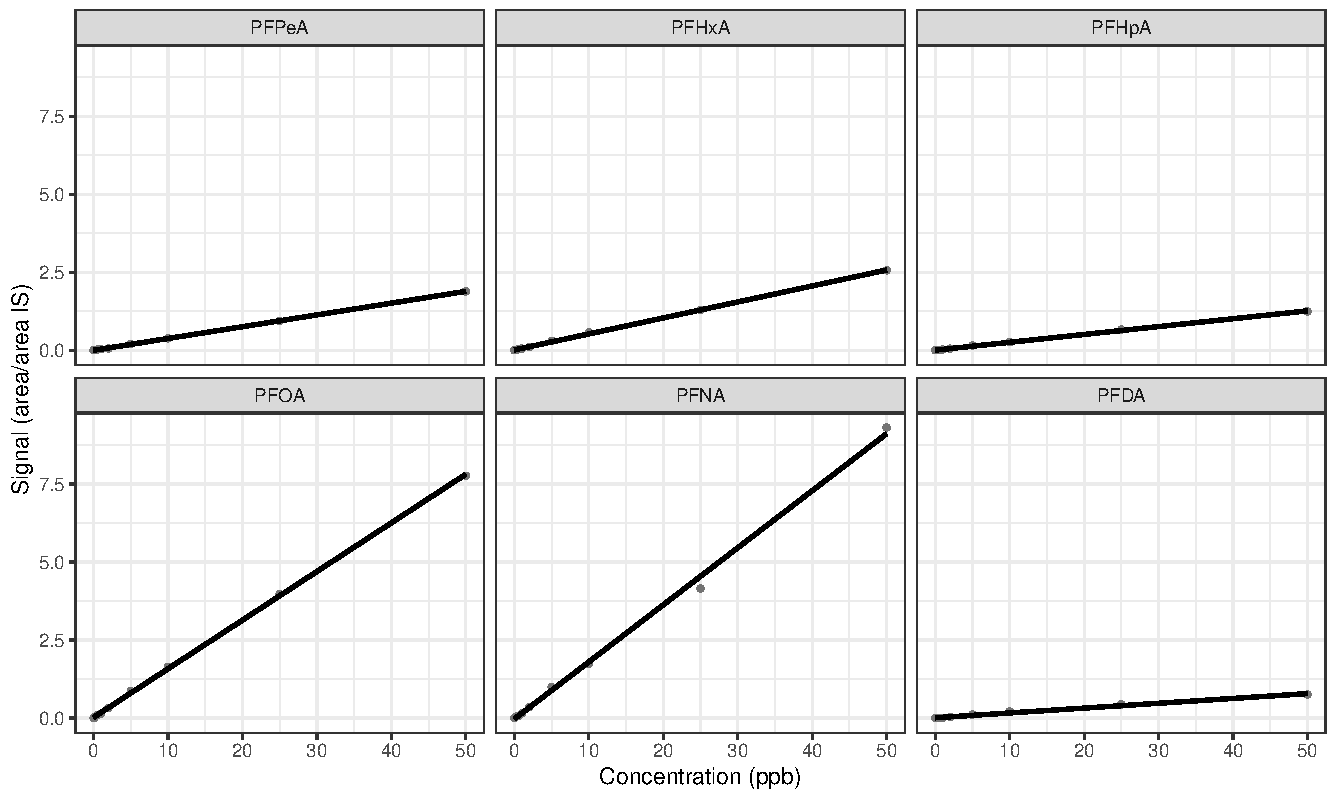
\includegraphics[width=\textwidth]{R/figs/CC_all.pdf}
    \caption{Calibration curve solvent blank}
    \label{appfig:CC}
\end{figure}

Matrix effect

\begin{figure}
    \centering
    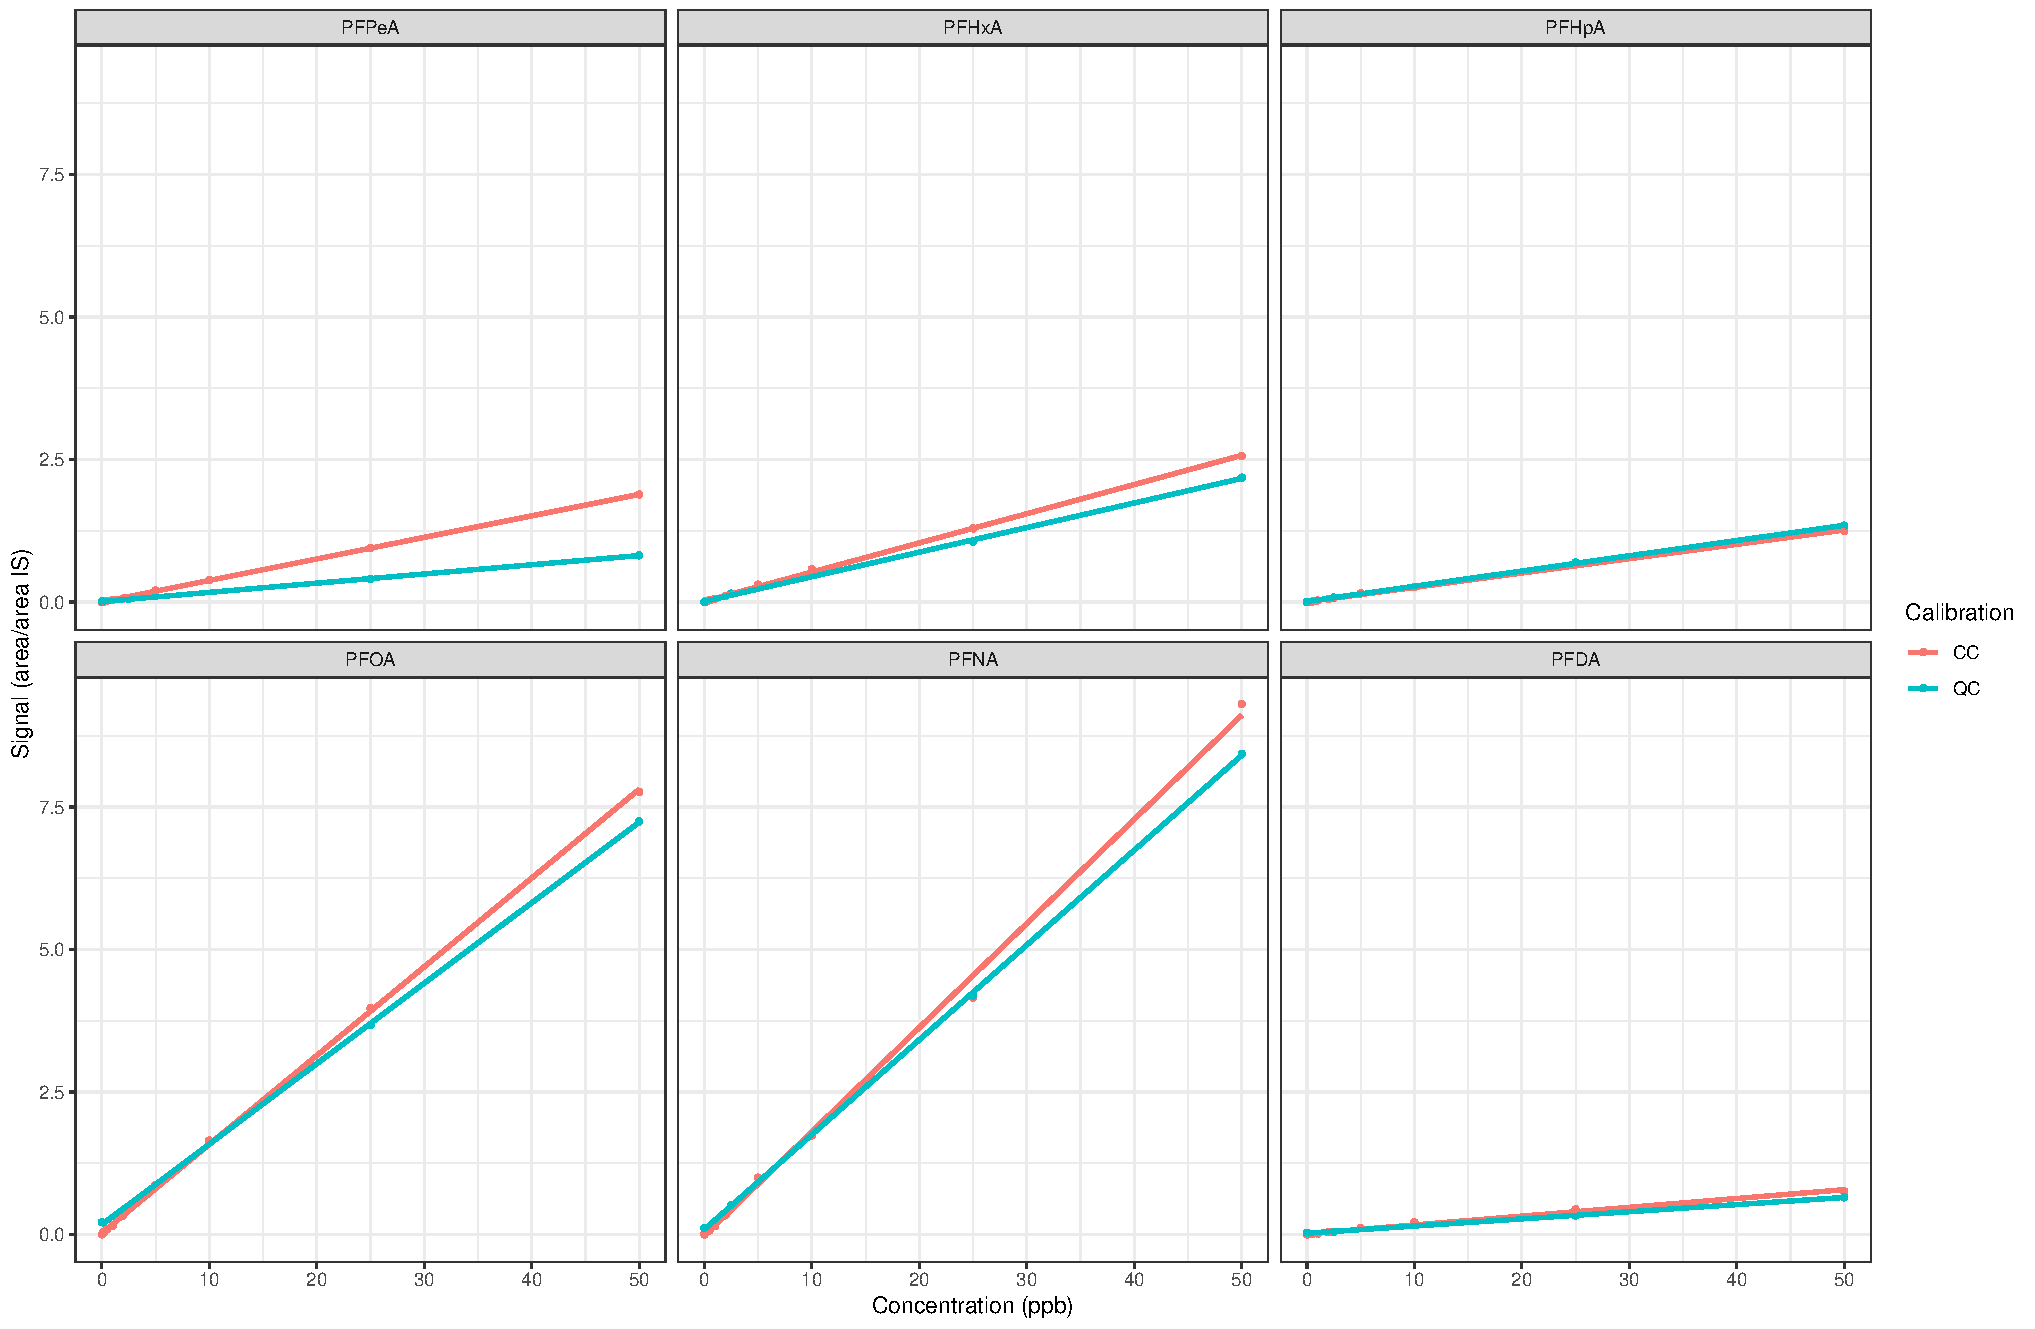
\includegraphics[width=\textwidth]{R/figs/CCQC_matrixeffect.pdf}
    \caption{Matrix effect (ME) for the PFCAs where CC = calibration curve in solvent blank, QC = matrix matched calibration curve. QC in line with CC indicates no ME, QC \textgreater CC = ion enhancement, CC \textless QC = ion suppression.}
    \label{appfig:ME}
\end{figure}
\chapter{Miscellaneous laboratory tests}\label{appSec:misclab}

In the following section, miscellaneous laboratory performed to strengthen the experimental certainty of the batch sorption isotherm tests are presented. 

\subsection{pH and conductivity}

\begin{figure} 
\centering
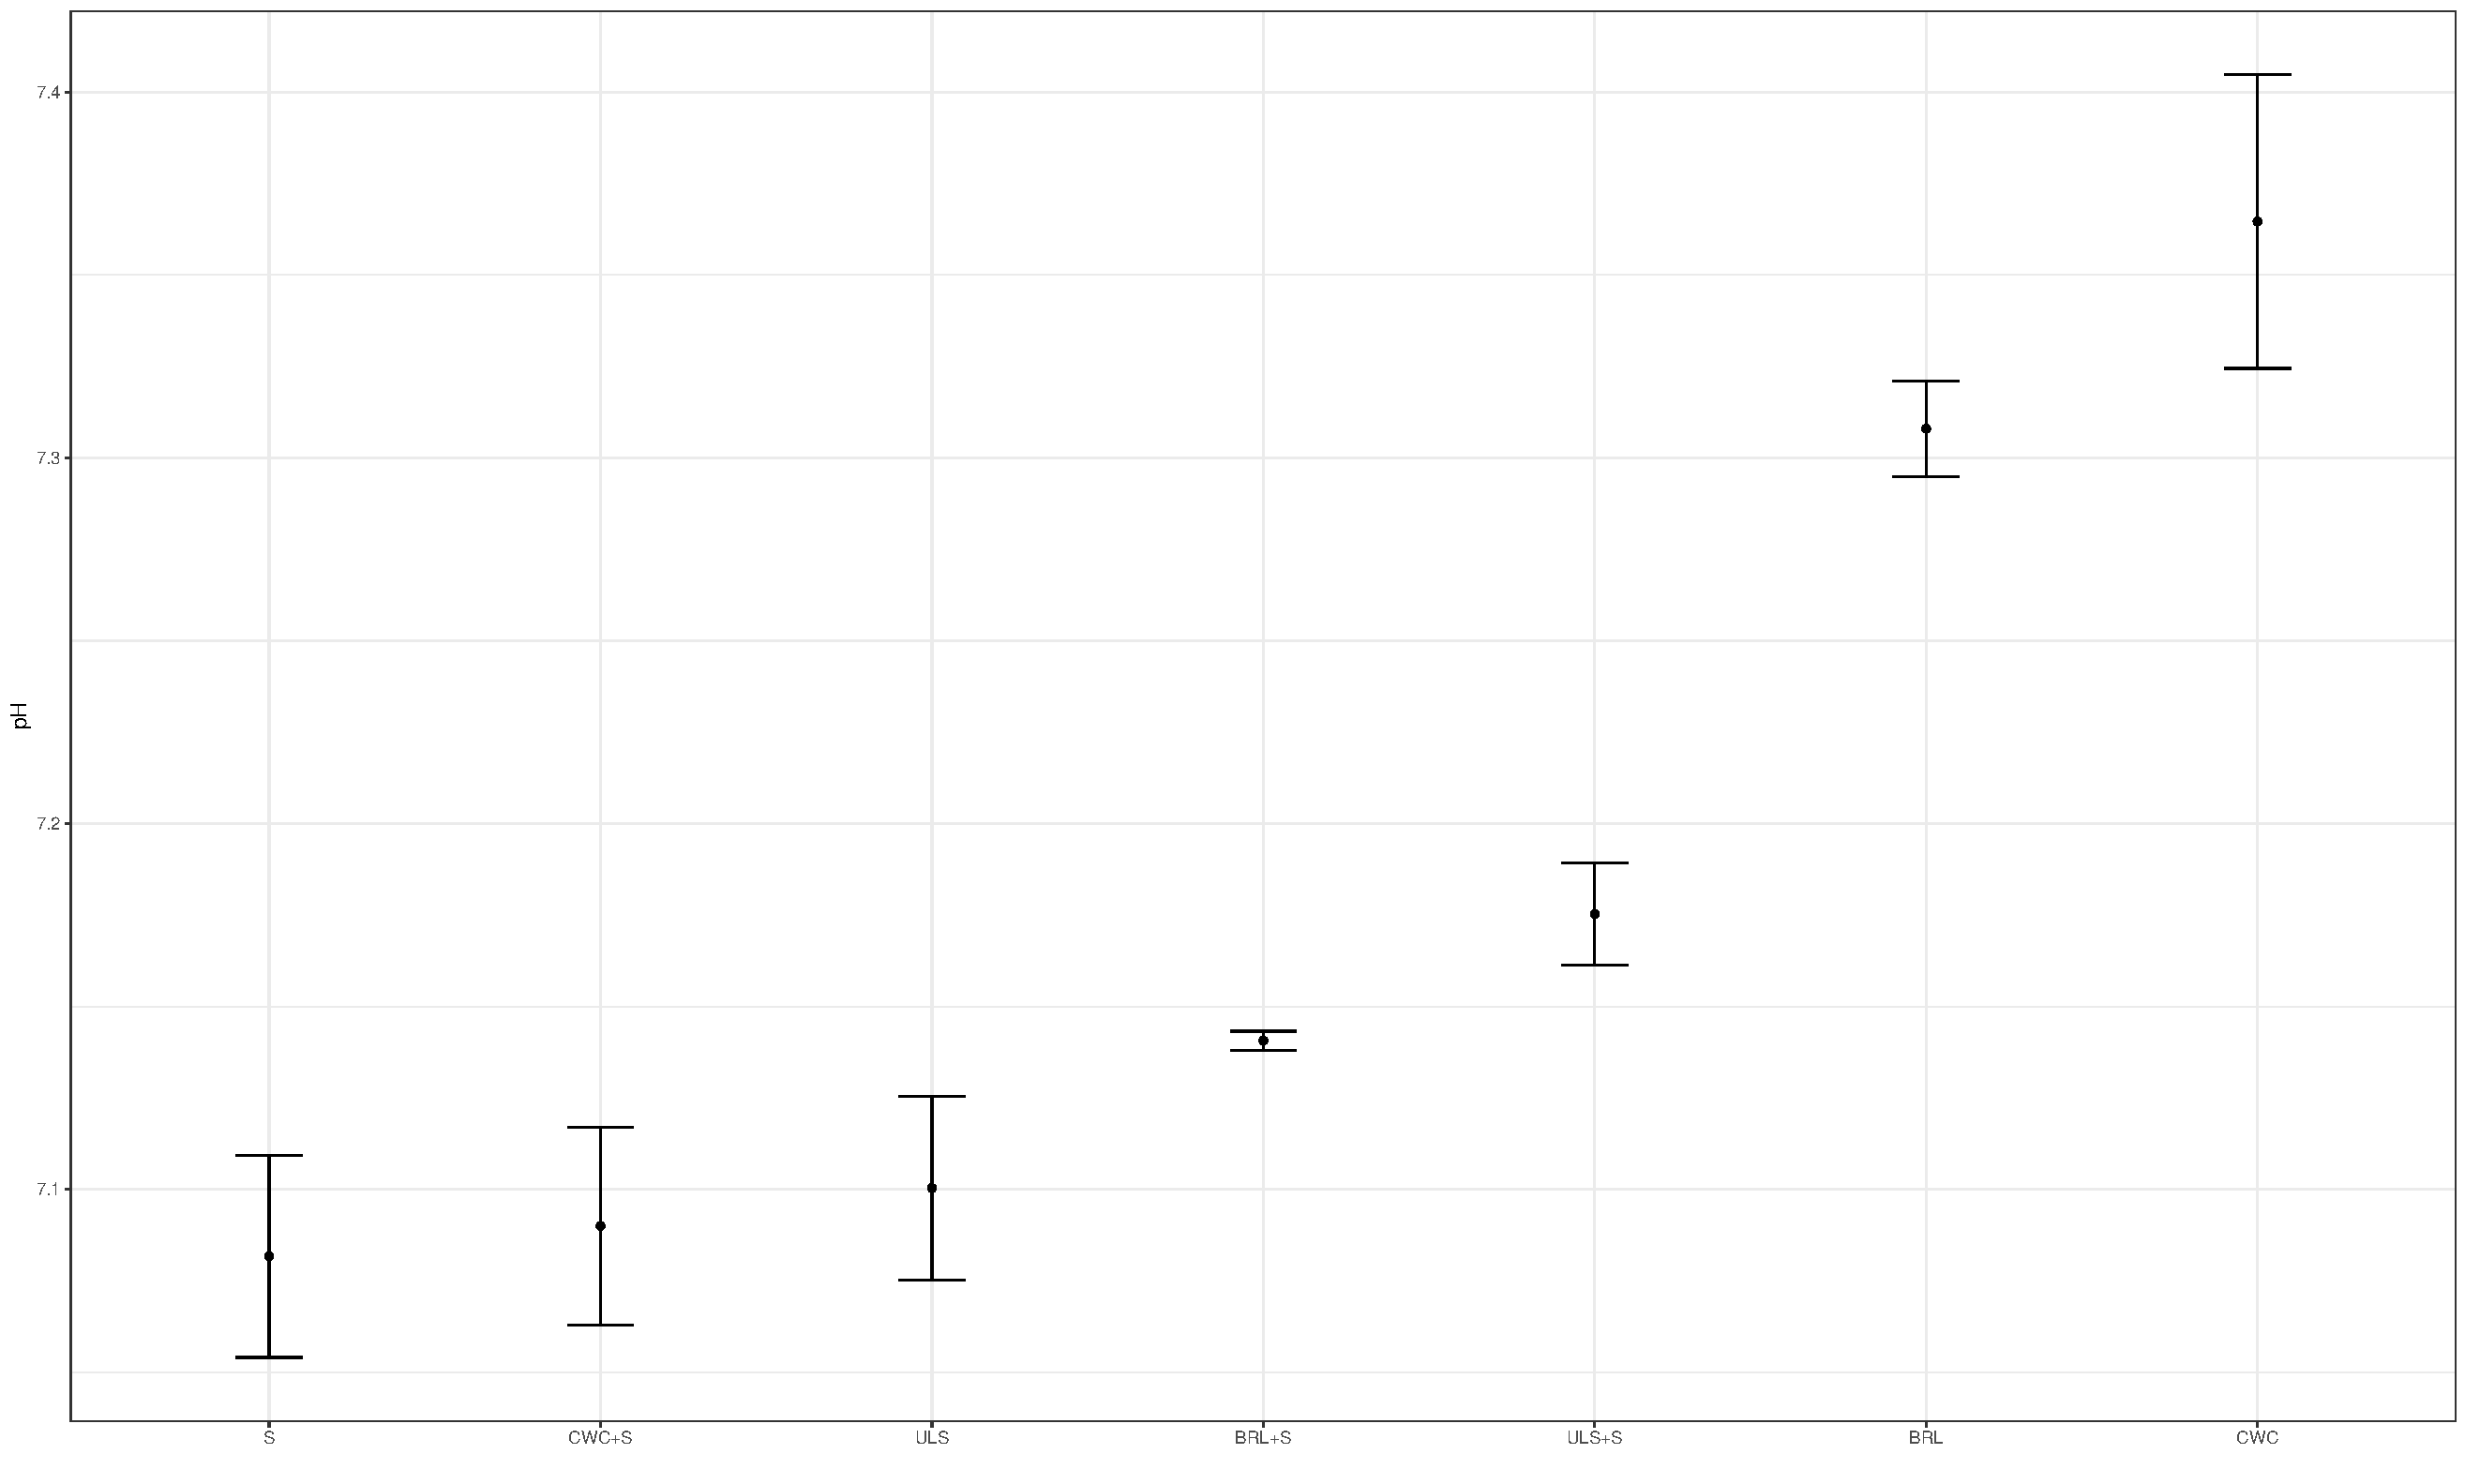
\includegraphics[width=\textwidth]{R/figs/pH.pdf}
\caption{Plot of pH measurements for 50 mL milli-Q water batch tests with 0.1 g biochars (CWC, ULS, BRL) and 5 g soil (S) (n=3).}
\label{appfig:pH}
\end{figure}

\begin{figure} 
\centering
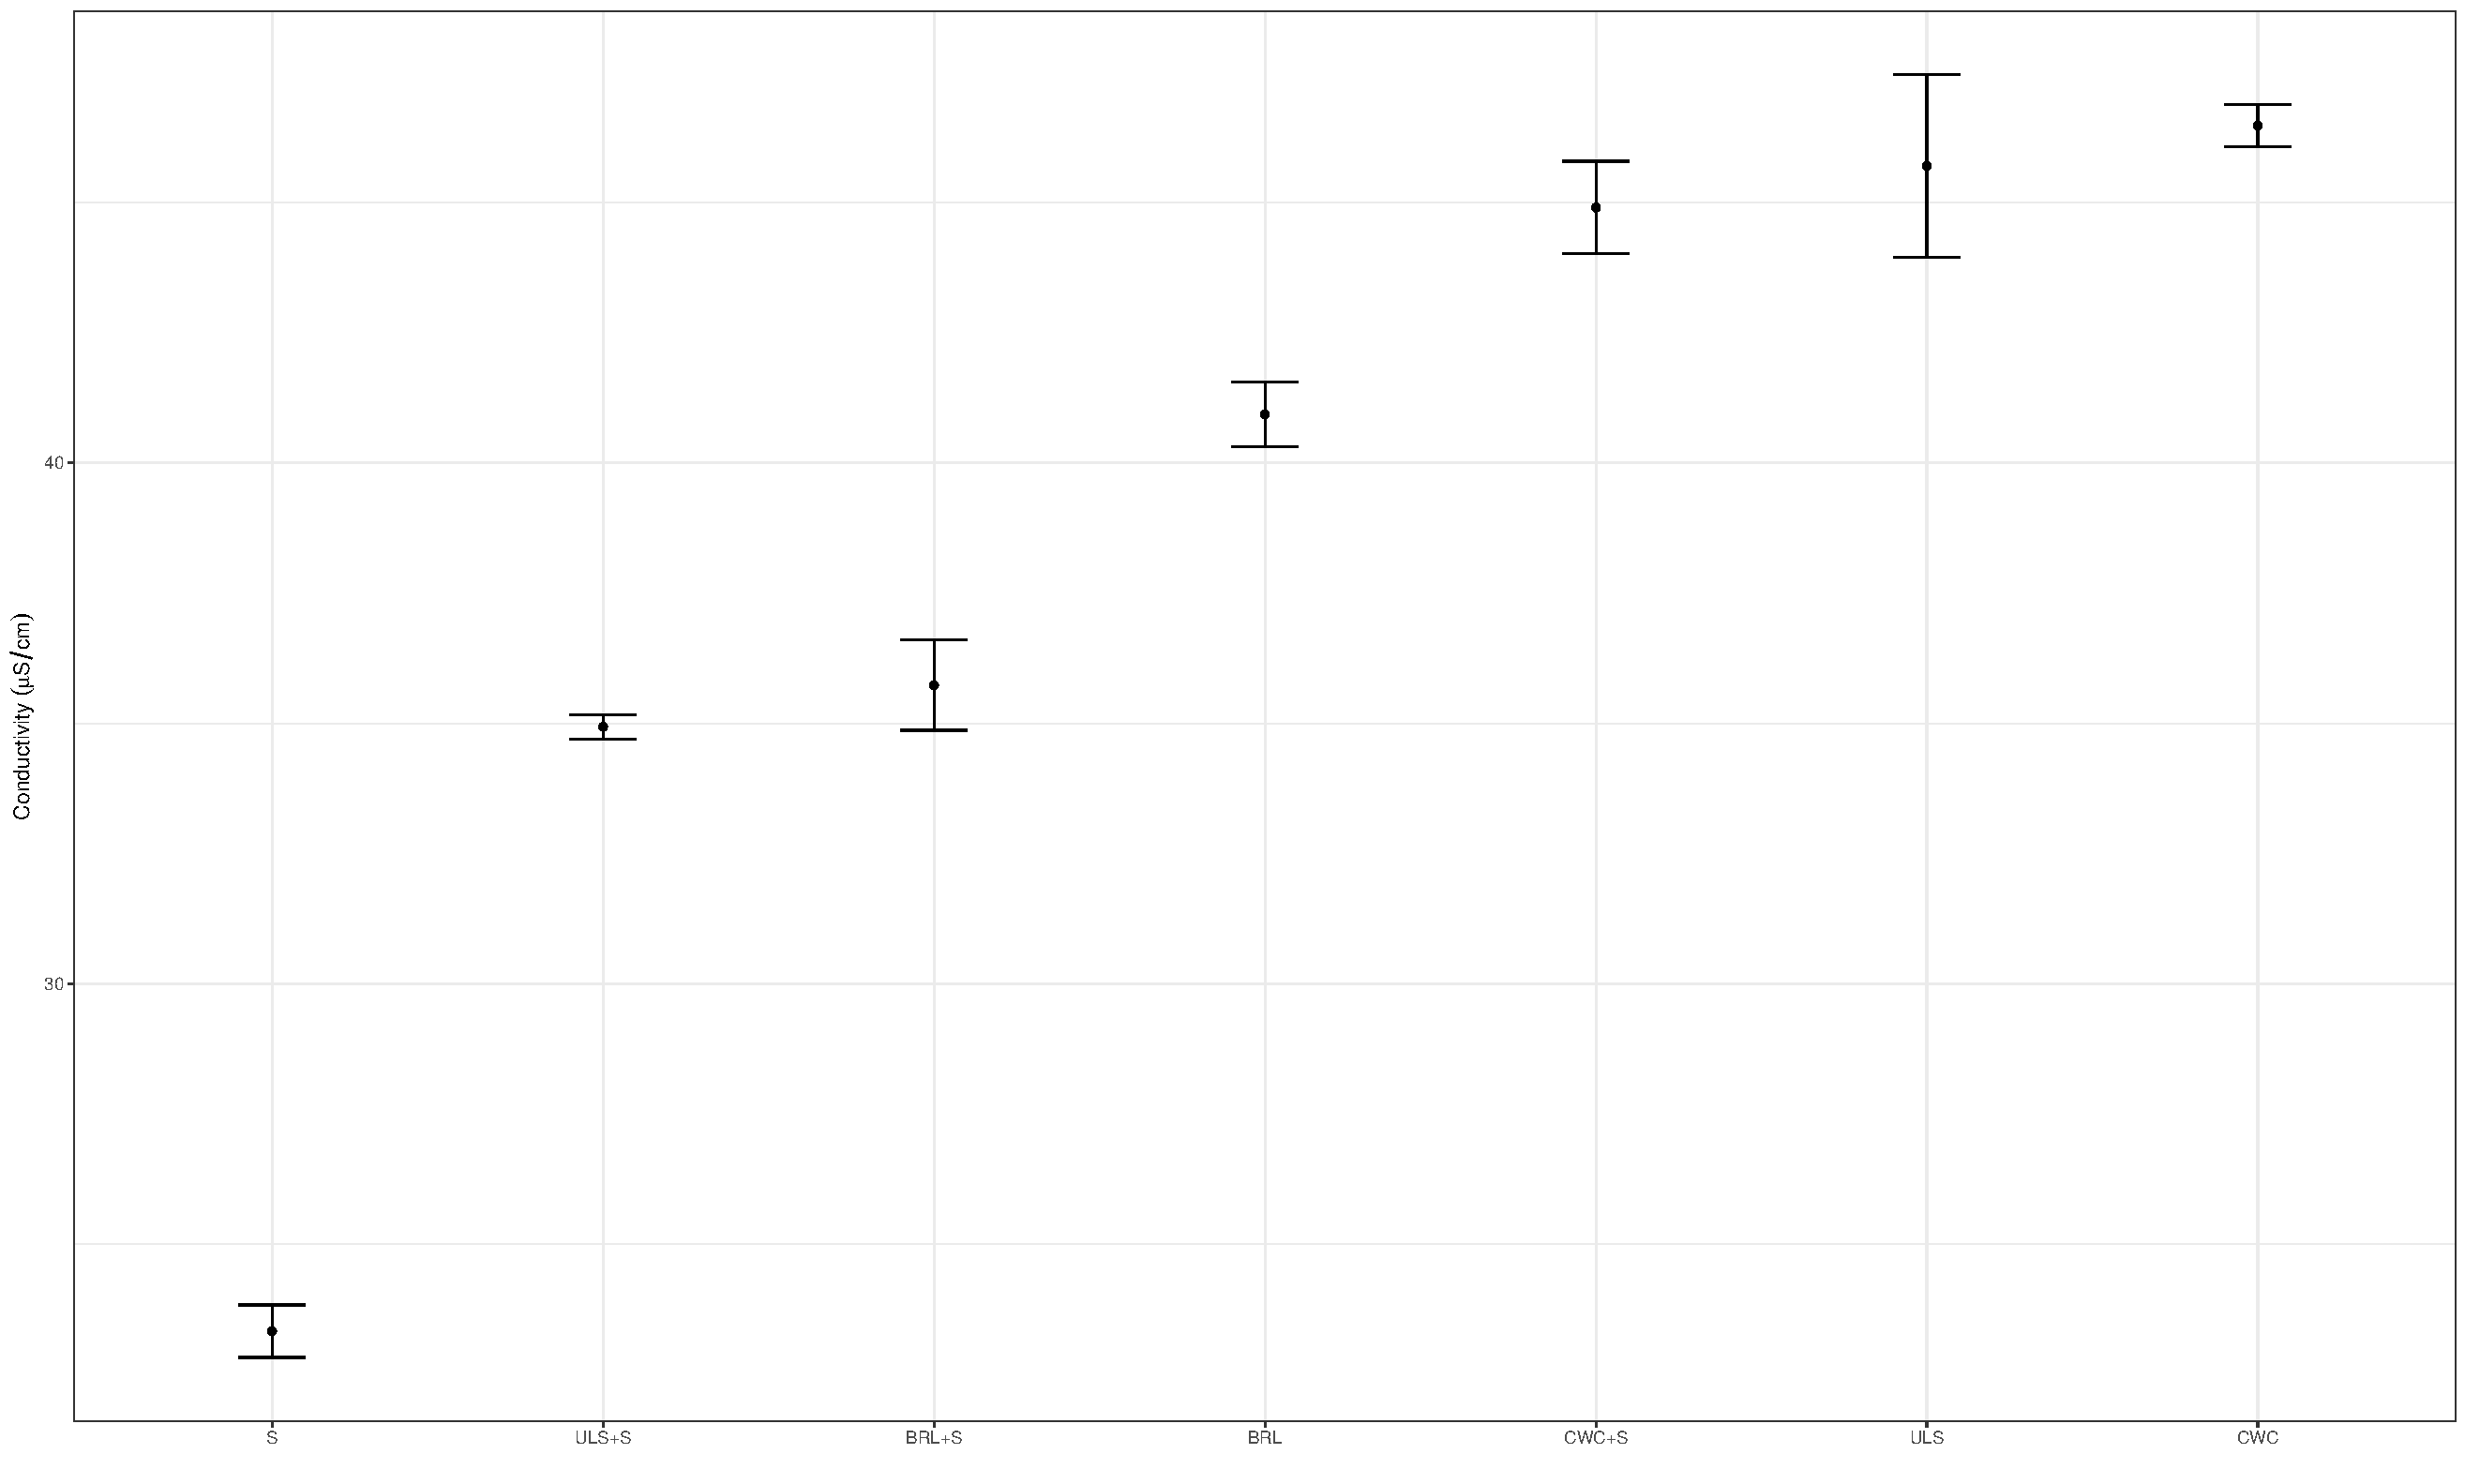
\includegraphics[width=\textwidth]{R/figs/conductivity.pdf}
\caption{Plot of conductivity measurements for 50 mL milli-Q water batch tests with 0.1 g biochars (CWC, ULS, BRL) and 5 g soil (S) (n=3).}
\label{appfig:cond}
\end{figure}

\begin{table}[h]
\centering
\caption{Pipette calibration for 2-10 mL pipette. PASS is given if CV $\leq$ 1.0 \% and the average volume dispensed is within 1.8400 - 2.1600 mL. }
\label{appTab:pip2-10}
\adjustbox{max width=\textwidth}{%
\begin{tabular}{lrrrrrrr} \toprule
 & \multicolumn{1}{l}{} &  &  &  & \multicolumn{3}{r}{Operator: Thermo Fishcer Scientific} \\
 & \multicolumn{1}{l}{} &  &  &  & \multicolumn{3}{r}{Serial number: EJ08813} \\
 & \multicolumn{1}{l}{} &  &  &  & \multicolumn{3}{r}{Date: 04.10.2021} \\ \midrule
\multicolumn{1}{c}{\textbf{\begin{tabular}[c]{@{}c@{}}Test volume\\ (mL)\end{tabular}}} & \multicolumn{1}{c}{\textbf{}} & \multicolumn{1}{c}{\textbf{\begin{tabular}[c]{@{}c@{}}Weight of\\ dispensed\\ volume (g)\end{tabular}}} & \multicolumn{1}{c}{\textbf{\begin{tabular}[c]{@{}c@{}}Corrected\\ volume (g)\end{tabular}}} & \multicolumn{1}{c}{\textbf{\begin{tabular}[c]{@{}c@{}}Average\\ volume (mL)\end{tabular}}} & \multicolumn{1}{c}{\textbf{SDEV}} & \multicolumn{1}{c}{\textbf{CV}} & \multicolumn{1}{c}{\textbf{PASS/FAIL}} \\ \midrule
\multicolumn{1}{c}{\textbf{2}} & \multicolumn{1}{c}{\textbf{}} &  &  & 2.0868 & 0.006 & 0.3 \% &  \\
\multicolumn{1}{c}{\textbf{}} & 1 & 2.0804 & 2.0842 &  &  &  &  \\
 & 2 & 2.0923 & 2.0961 &  &  &  &  \\
 & 3 & 2.0902 & 2.0940 &  &  &  &  \\
 & 4 & 2.0861 & 2.0899 &  &  &  &  \\
 & 5 & 2.0817 & 2.0855 &  &  &  &  \\
 & 6 & 2.0852 & 2.0890 &  &  &  &  \\
 & 7 & 2.0807 & 2.0845 &  &  &  &  \\
 & 8 & 2.0829 & 2.0867 &  &  &  &  \\
 & 9 & 2.0778 & 2.0815 &  &  &  & \textbf{} \\
 & 10 & 2.0727 & 2.0764 &  &  &  &  \\
 & \multicolumn{1}{l}{} &  &  & \textbf{} & \textbf{} &  & \cellcolor[HTML]{C0C0C0}\textbf{PASS} \\ \bottomrule
\end{tabular}}
\end{table}



\begin{table}
\centering
\caption{Pipette calibration for 200-1000 μL pipette. PASS is given if CV $\leq$ 1.0 \% and the average volume dispensed is within 992 - 1008 μL. }
\label{appTab:pip200-1000}
\adjustbox{max width=\textwidth}{%
\begin{tabular}{lrrrrrrr} \toprule
 & \multicolumn{1}{l}{} & \multicolumn{1}{l}{} & \multicolumn{1}{l}{} & \multicolumn{1}{l}{} & \multicolumn{3}{r}{Operator: Thermo Fischer Scientific} \\
 & \multicolumn{1}{l}{} & \multicolumn{1}{l}{} & \multicolumn{1}{l}{} & \multicolumn{1}{l}{} & \multicolumn{3}{r}{Serial Number: EH23798 4500} \\
 & \multicolumn{1}{l}{} & \multicolumn{1}{l}{} & \multicolumn{1}{l}{} & \multicolumn{1}{l}{} & \multicolumn{3}{r}{Date: 04.10.2021} \\ \midrule
\multicolumn{1}{c}{\textbf{\begin{tabular}[c]{@{}c@{}}Test volume \\ (μL)\end{tabular}}} & \textbf{} & \multicolumn{1}{c}{\textbf{\begin{tabular}[c]{@{}c@{}}Weight of\\ dispensed\\ volume (g)\end{tabular}}} & \multicolumn{1}{c}{\textbf{\begin{tabular}[c]{@{}c@{}}Corrected\\ volume (μL)\end{tabular}}} & \multicolumn{1}{c}{\textbf{\begin{tabular}[c]{@{}c@{}}Average\\ volume (μL)\end{tabular}}} & \multicolumn{1}{c}{\textbf{SDEV}} & \multicolumn{1}{c}{\textbf{CV}} & \multicolumn{1}{c}{\textbf{PASS/FAIL}} \\ \midrule
\multicolumn{1}{c}{\textbf{1000}} & \textbf{} & \multicolumn{1}{l}{} & \multicolumn{1}{l}{} & 994.2 & 5 & 0.5 \% & \multicolumn{1}{l}{} \\
\multicolumn{1}{c}{} & 1 & 997.0 & 998.8 &  &  &  &  \\
 & 2 & 999.4 & 1001.2 &  &  &  &  \\
 & 3 & 990.4 & 992.2 &  &  &  &  \\
 & 4 & 992.3 & 994.1 &  &  &  &  \\
 & 5 & 990.5 & 992.3 &  &  &  &  \\
 & 6 & 990.9 & 992.7 &  &  &  &  \\
 & 7 & 983.8 & 985.6 &  &  &  &  \\
 & 8 & 990.9 & 992.7 &  &  &  &  \\
 & 9 & 990.5 & 992.3 &  &  &  &  \\
 & 10 & 998.4 & 1000.2 &  &  &  &  \\
 & \multicolumn{1}{l}{} & \multicolumn{1}{l}{} & \multicolumn{1}{l}{} & \multicolumn{1}{l}{\textbf{}} & \multicolumn{1}{l}{\textbf{}} & \multicolumn{1}{l}{} & \multicolumn{1}{l}{\cellcolor[HTML]{C0C0C0}\textbf{PASS}} \\ \bottomrule
\end{tabular}}
\end{table}


\begin{table}
\centering
\caption{Pipette calibration for 5 - 50 μL pipette. PASS is given if CV $\leq$ 2.5 \% and the average volume dispensed is within 19.8 - 20.2 μL. }
\label{appTab:pip5-50}
\adjustbox{max width=\textwidth}{%
\begin{tabular}{lrrrrrrr} \toprule
 & \multicolumn{1}{l}{} & \multicolumn{1}{l}{} & \multicolumn{1}{l}{} & \multicolumn{1}{l}{} & \multicolumn{3}{r}{Operator: Thermo Fischer Scientific} \\
 & \multicolumn{1}{l}{} & \multicolumn{1}{l}{} & \multicolumn{1}{l}{} & \multicolumn{1}{l}{} & \multicolumn{3}{r}{Serial Number: EH94947 4500} \\
 & \multicolumn{1}{l}{} & \multicolumn{1}{l}{} & \multicolumn{1}{l}{} & \multicolumn{1}{l}{} & \multicolumn{3}{r}{Date: 04.10.2021} \\ \midrule
\multicolumn{1}{c}{\textbf{\begin{tabular}[c]{@{}c@{}}Test volume\\ (μL)\end{tabular}}} & \multicolumn{1}{c}{\textbf{}} & \multicolumn{1}{c}{\textbf{\begin{tabular}[c]{@{}c@{}}Weight of\\ dispensed\\ volume (g)\end{tabular}}} & \multicolumn{1}{c}{\textbf{\begin{tabular}[c]{@{}c@{}}Corrected\\ volume (mL)\end{tabular}}} & \multicolumn{1}{c}{\textbf{\begin{tabular}[c]{@{}c@{}}Average\\ volume (mL)\end{tabular}}} & \multicolumn{1}{c}{\textbf{SDEV}} & \multicolumn{1}{c}{\textbf{CV}} & \multicolumn{1}{c}{\textbf{PASS/FAIL}} \\ \midrule
\multicolumn{1}{c}{\textbf{20}} & &  &  & 19.8 & 0.4 & 2 $\%$ & \multicolumn{1}{l}{} \\
 & 1 & 19.8 & 19.8 &  &  &  &  \\
 & 2 & 19.5 & 19.5 &  &  &  &  \\
 & 3 & 19.8 & 19.8 &  &  &  &  \\
 & 4 & 20.8 & 20.8 &  &  &  &  \\
 & 5 & 19.9 & 19.9 &  &  &  &  \\
 & 6 & 19.6 & 19.6 &  &  &  &  \\
 & 7 & 19.7 & 19.7 &  &  &  &  \\
 & 8 & 19.5 & 19.5 &  &  &  &  \\
 & 9 & 19.2 & 19.2 &  &  &  &  \\
 & 10 & 19.9 & 19.9 &  &  &  & \cellcolor[HTML]{FFFFFF}\textbf{} \\
 & \multicolumn{1}{l}{} & \multicolumn{1}{l}{} & \multicolumn{1}{l}{} &  &  &  & \multicolumn{1}{l}{\cellcolor[HTML]{C0C0C0}\textbf{PASS}} \\ \bottomrule
\end{tabular}}
\end{table}

\begin{table}
\centering
\caption{Volume calibration for 50 mL Falcon high-clarity polypropylene (PP) conical centrifuge tube. PASS is given if CV $\leq$ and the average volume filled is within 49.0 - 51.0 mL.}
\label{appTab:PPcentrifuge}
\adjustbox{max width=\textwidth}{%
\begin{tabular}{crrrrrrrr} \toprule
 &  &  &  &  & \multicolumn{4}{r}{Date: 26.10.2021} \\ \midrule
\multicolumn{1}{c}{\textbf{\begin{tabular}[c]{@{}c@{}}Test\\volume (mL)\end{tabular}}} & \multicolumn{1}{c}{\textbf{}} & \multicolumn{1}{c}{\textbf{\begin{tabular}[c]{@{}c@{}}Initial \\ weight  (g)\end{tabular}}} & \multicolumn{1}{c}{\textbf{\begin{tabular}[c]{@{}c@{}}Final\\weight (g)\end{tabular}}} & \multicolumn{1}{c}{\textbf{\begin{tabular}[c]{@{}c@{}}Net \\weight (g)\end{tabular}}} & \multicolumn{1}{c}{\textbf{\begin{tabular}[c]{@{}c@{}}Average \\ volume (mL)\end{tabular}}} & \multicolumn{1}{c}{\textbf{SDEV}} & \multicolumn{1}{c}{\textbf{CV}} & \multicolumn{1}{c}{\textbf{PASS/FAIL}} \\ \midrule
\textbf{50} &  &  &  &  & 48.4756 & 0.2 & 0.4 \% &  \\
 & 1 & 13.0354 & 61.3521 & 48.3167 &  &  &  &  \\
 & 2 & 13.0572 & 61.3498 & 48.2926 &  &  &  &  \\
 & 3 & 13.0154 & 61.1161 & 48.1007 &  &  &  &  \\
 & 4 & 13.0857 & 61.8386 & 48.7529 &  &  &  &  \\
 & 5 & 13.0658 & 61.6241 & 48.5583 &  &  &  &  \\
 & 6 & 12.9908 & 61.6972 & 48.7064 &  &  &  &  \\
 & 7 & 13.0073 & 61.4474 & 48.4401 &  &  &  &  \\
 & 8 & 13.0699 & 61.7248 & 48.6549 &  &  &  &  \\
 & 9 & 12.7855 & 61.3788 & 48.5933 &  &  &  &  \\
 & 10 & 12.9962 & 61.3365 & 48.3403 &  &  &  &  \\
 &  &  &  &  &  &  &  & \multicolumn{1}{l}{\cellcolor[HTML]{C0C0C0}\textbf{FAIL}} \\ \bottomrule
\end{tabular}}
\end{table}

\begin{table}
\centering
\caption{Mass CWC left in syringe after filtering of biochar-PFCA solution. Total mass CWC is 0.1000 $\pm$ 0.004 g.}
\label{appTab:CWCloss}
\begin{tabular}{rrrrr} \toprule
 & Mass (g) & \multicolumn{1}{c}{$\bar{x}$} & \multicolumn{1}{c}{SDEV} & \multicolumn{1}{c}{CV}  \\ \midrule
 & & 0.0488 & 0.003 & 8 $\%$ \\
1 & 0.0429 \\
2 & 0.0413 \\
3 & 0.0484 \\
4 & 0.0428 \\
5 & 0.0485 \\ \bottomrule
\end{tabular}
\end{table}

Here can include soil precipitation test?


\chapter{Element analysis soil and biochar}\label{appSec:elements}

\begin{table}
\centering
\caption{Total element composition of the biochars used in this thesis.}
\adjustbox{max width=\textwidth}{
\label{apptab:totelem}
\begin{threeparttable}
\begin{tabular}{lccccccc} 
\toprule
\textbf{}                   & \textbf{} & \multicolumn{2}{c}{\textbf{CWC}} & \multicolumn{2}{c}{\textbf{ULS}} & \multicolumn{2}{c}{\textbf{DSL}} \\ \cline{3-8} 
                                       &           & Mean              & Std.dev          & Mean             & Std.dev           & Mean            & Std.dev            \\ \hline \addlinespace
\textbf{Main elements} &&&&&&& \\ \hline \addlinespace
C                                       & \%        & 91.4              & 2.5              & 29.63            & 0.47              & 13.5            & 0.2                \\
N                                       & \%        & 0.69              & 0.02             & 1.131            & 0.039             & 0.82            & 0.02               \\
H                                       & \%        & 1.01              & 0.14             & 1.243            & 0.045             & 1.05            & 0.16               \\
O\textsuperscript{*}                            & \%        &     5.5              &                  &       57.1           &                   &        61.4         &                    \\
Ca                        & g/kg      & 8.0               & 0.2              & 21               &                   & 26.0            & 0.0                \\
Fe                        & g/kg      & 0.13              & 0.04             & 23               &                   & 180             & 0                  \\
K                         & g/kg      & 4.03              & 0.06             & 6.8              &                   & 3.7             & 0.1                \\
Mg                        & g/kg      & 0.91              & 0.02             & 5.3              &                   & 4.70            & 0.17               \\
Na                         & g/kg      & 0.05              & 0.00             & 2.4              &                   & 1.83            & 0.06               \\
P                          & g/kg      & 0.41              & 0.01             & 45               &                   & 8.0             & 0.5                \\
S                         & g/kg      & 0.09              & 0.00             & 2.9              &                   & 7.23            & 0.68               \\
Si                         & g/kg      & 0.17              & 0.02             & 1.7              &                   & 0.62            & 0.08               \\ \addlinespace \hline \addlinespace
\textbf{Trace elements} &&&&&&&    \\ \hline \addlinespace
As                         & mg/kg     & 0.01              & 0.00             & 3.0              &                   & 3.13            & 0.21               \\
Ba                        & mg/kg     & 216.67            & 5.77             & 310              &                   & 177             & 6                  \\
Cd                        & mg/kg     & 0.00044           & -                & 0.0081           &                   & 0.03            & 0.00               \\
Co                        & mg/kg     & 0.30              & 0.03             & 7.1              &                   & 9.97            & 0.06               \\
Cr                        & mg/kg     & 1.69              & 1.22             & 56               &                   & 53.3            & 1.5                \\
Cu                        & mg/kg     & 5.17              & 0.60             & 220              &                   & 277             & 6                  \\
Mo                       & mg/kg     & 0.06              & 0.02             & 7.1              &                   & 19.0            & 0.0                \\
Ni                        & mg/kg     & 1.77              & 0.64             & 41               &                   & 34.7            & 0.6                \\
Pb                       & mg/kg     & 0.08              & 0.02             & 13               &                   & 25.3            & 4.0                \\
Sr                        & mg/kg     & 36                & 2                & 87               &                   & 120             & 0                  \\
V                         & mg/kg     & 0.10              & 0.02             & 34               &                   & 54.0            & 1.0                \\
Zn                        & mg/kg     & 3.2               & 0.6              & 480              &                   & 0.80            & 0.01      \\ \bottomrule   
\end{tabular}
\begin{tablenotes}
\item \textsuperscript{*} Calculated as remaining fraction after subtraction of all other elements listed.
\end{tablenotes}
\end{threeparttable}}
\end{table}

\begin{table}
\centering
\caption{Total concentration, exchangeable ions and summary parameters for the soil used in the batch leaching tests. Total concentrations are in mg/kg d.w.}
\label{apptab:soil}
\begin{tabular}{lccc}
\toprule
\multicolumn{1}{l}{\textbf{Main parameters}}          &                               & \textbf{Mean}                          & \textbf{Std. Dev}                      \\ \hline \addlinespace
pH (H\textsubscript{2}O)                      &                               & 5.38                          & 0.02                          \\
pH (0.01 M CaCl\textsubscript{2})             &                               & 4.36                          & 0.01                          \\
C-org                         & \%                            & 1.32                          & 0.03                          \\
N-tot                         & \%                            & 0.11                          & 0.003                         \\ \hline
\textbf{Exchangeable ions}    & \multicolumn{1}{l}{\textbf{}} & \multicolumn{1}{l}{\textbf{}} & \multicolumn{1}{l}{\textbf{}} \\ \hline \addlinespace
Al\textsuperscript{3+}                          & meqv/100g                     & 0.87                          & 0.01                          \\
H\textsuperscript{+}                            & meqv/100g                     & 0.09                          & 0.03                          \\
Mg\textsuperscript{2+}                          & meqv/100g                     & 0.07                          & 0.001                         \\
Ca\textsuperscript{2+}                          & meqv/100g                     & 1.54                          & 0.03                          \\
Na\textsuperscript{+}                           & meqv/100g                     & 0.01                          & 0.0004                        \\
K\textsuperscript{+}                            & meqv/100g                     & 0.05                          & 0.0002                        \\
CEC                           & meqv/100g                     & 2.63                          & 0.06                          \\ \hline
\textbf{Total concentrations} & \multicolumn{1}{l}{\textbf{}} & \multicolumn{1}{l}{\textbf{}} & \multicolumn{1}{l}{\textbf{}} \\ \hline \addlinespace
Ba                            & mg/kg                         & 11.03                         & 0.3                           \\
Be                            & mg/kg                         & 0.27                          & 0.004                         \\
Cd                            & mg/kg                         & 0.20                          & 0.06                          \\
Co                            & mg/kg                         & 2.07                          & 0.09                          \\
Cr                            & mg/kg                         & 6.13                          & 0.4                           \\
Cu                            & mg/kg                         & 9.10                          & 1.1                           \\
Fe                            & mg/kg                         & 6740.00                       & 445.4                         \\
Hg                            & mg/kg                      & \textless{}1                  &                               \\
Mn                            & mg/kg                      & 123.67                        & 6.8                           \\
Ni                            & mg/kg                      & 3.09                          & 0.2                           \\
P                             & mg/kg                      & 525.33                        & 29.3                          \\
Pb                            & mg/kg                      & 8.45                          & 0.5       \\ \bottomrule          
\end{tabular}
\end{table}
\chapter{Pollution control ETIA}\label{appSec:pollution}

In this chapter, additional work on gas emission environmental pollutant characterization is presented. The work was conducted during pyrolysis of digested sludge Lindum (DSL) and measured

Gas measurements have been performed of the gases that are emitted through the chimney. Measurements were performed by the author together with Erlend S\o rmo as an additional learning activity for this master thesis. Measurements included Hg using what instrument, PM10 and syn-gases using FTIR.

The ETIA measurement campaign started September 16, 2021 and aimed to measure emission of environmental pollutants from pyrolysis of the various feedstock types produced at Lindum AS. Included in the campaign are Hg, PM$_{10}$, qualitative analysis of syn-gas using FTIR, quantitative analysis of syn-gas using Low Volume / Medium Volume Sampler LVS / MVS for organic and inorganic pollutants. 


\begin{figure}
    \centering
    \begin{subfigure}[t]{\textwidth}
         \centering
         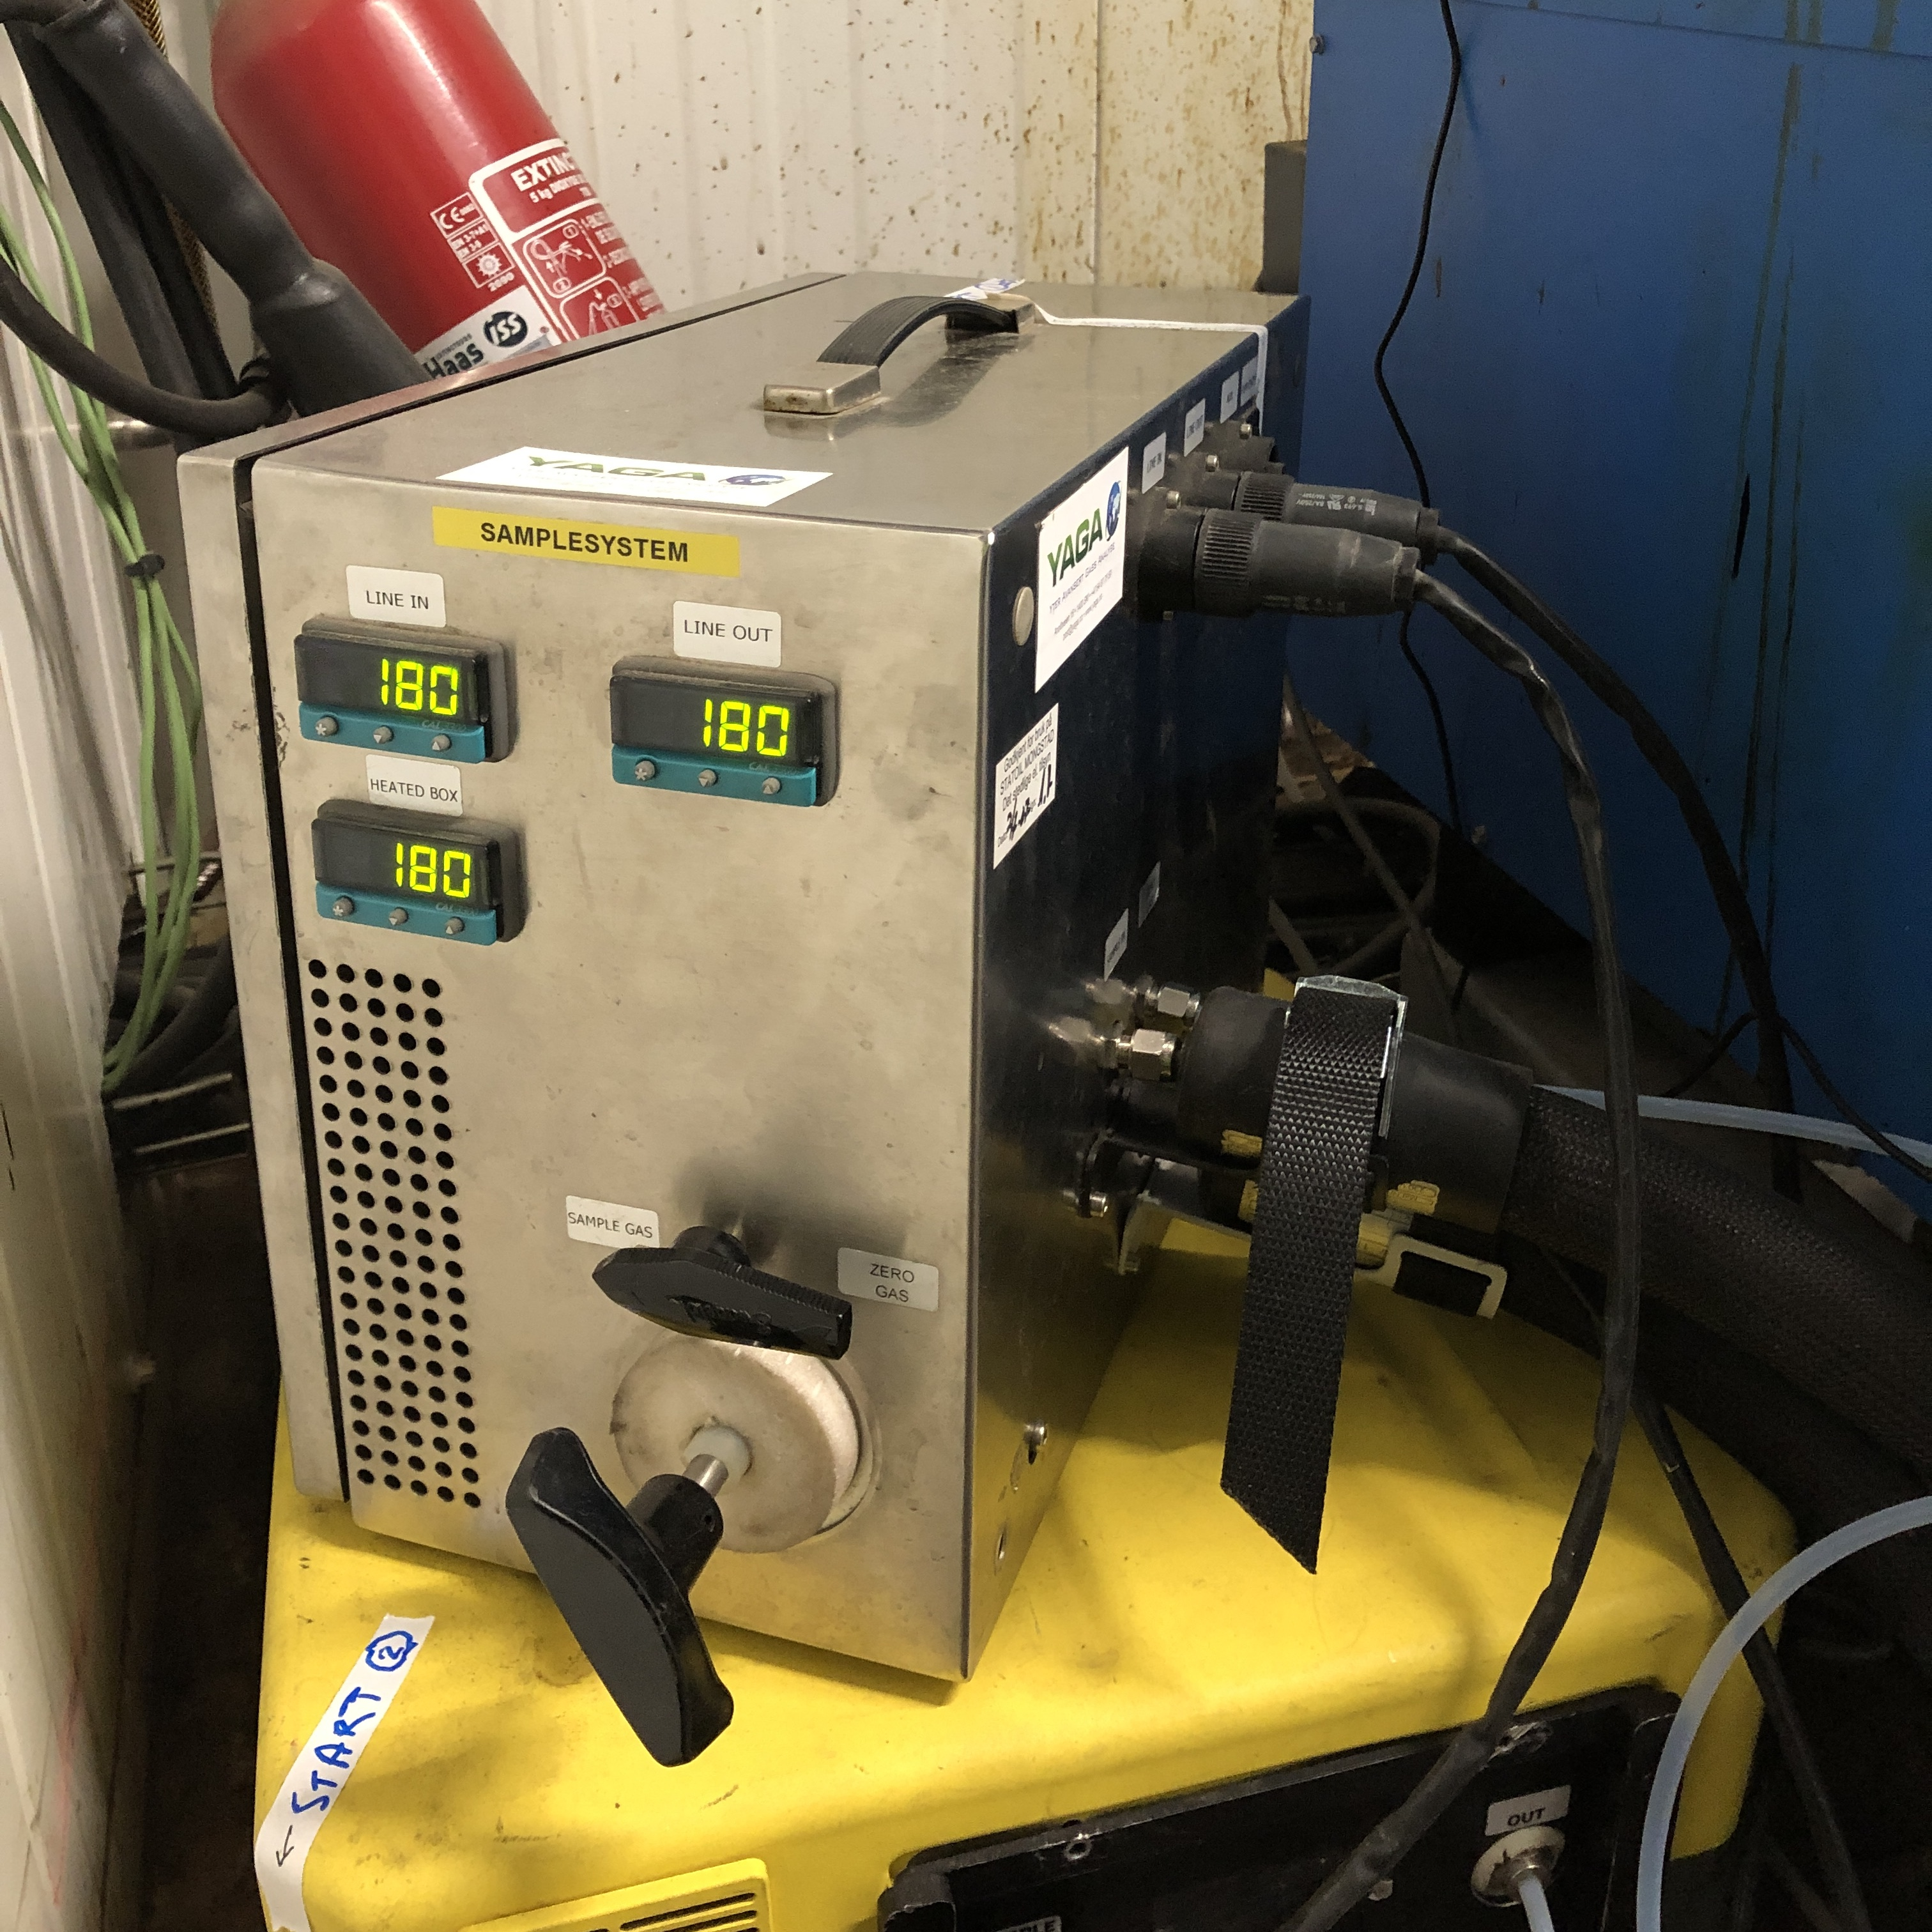
\includegraphics[width=0.6\textwidth]{Bilder/Pyrolysis/FTIR.jpg}
         \caption{}
         \label{appFig:FTIRbox}
     \end{subfigure}
     \hfill
     \begin{subfigure}[t]{\textwidth}
         \centering
         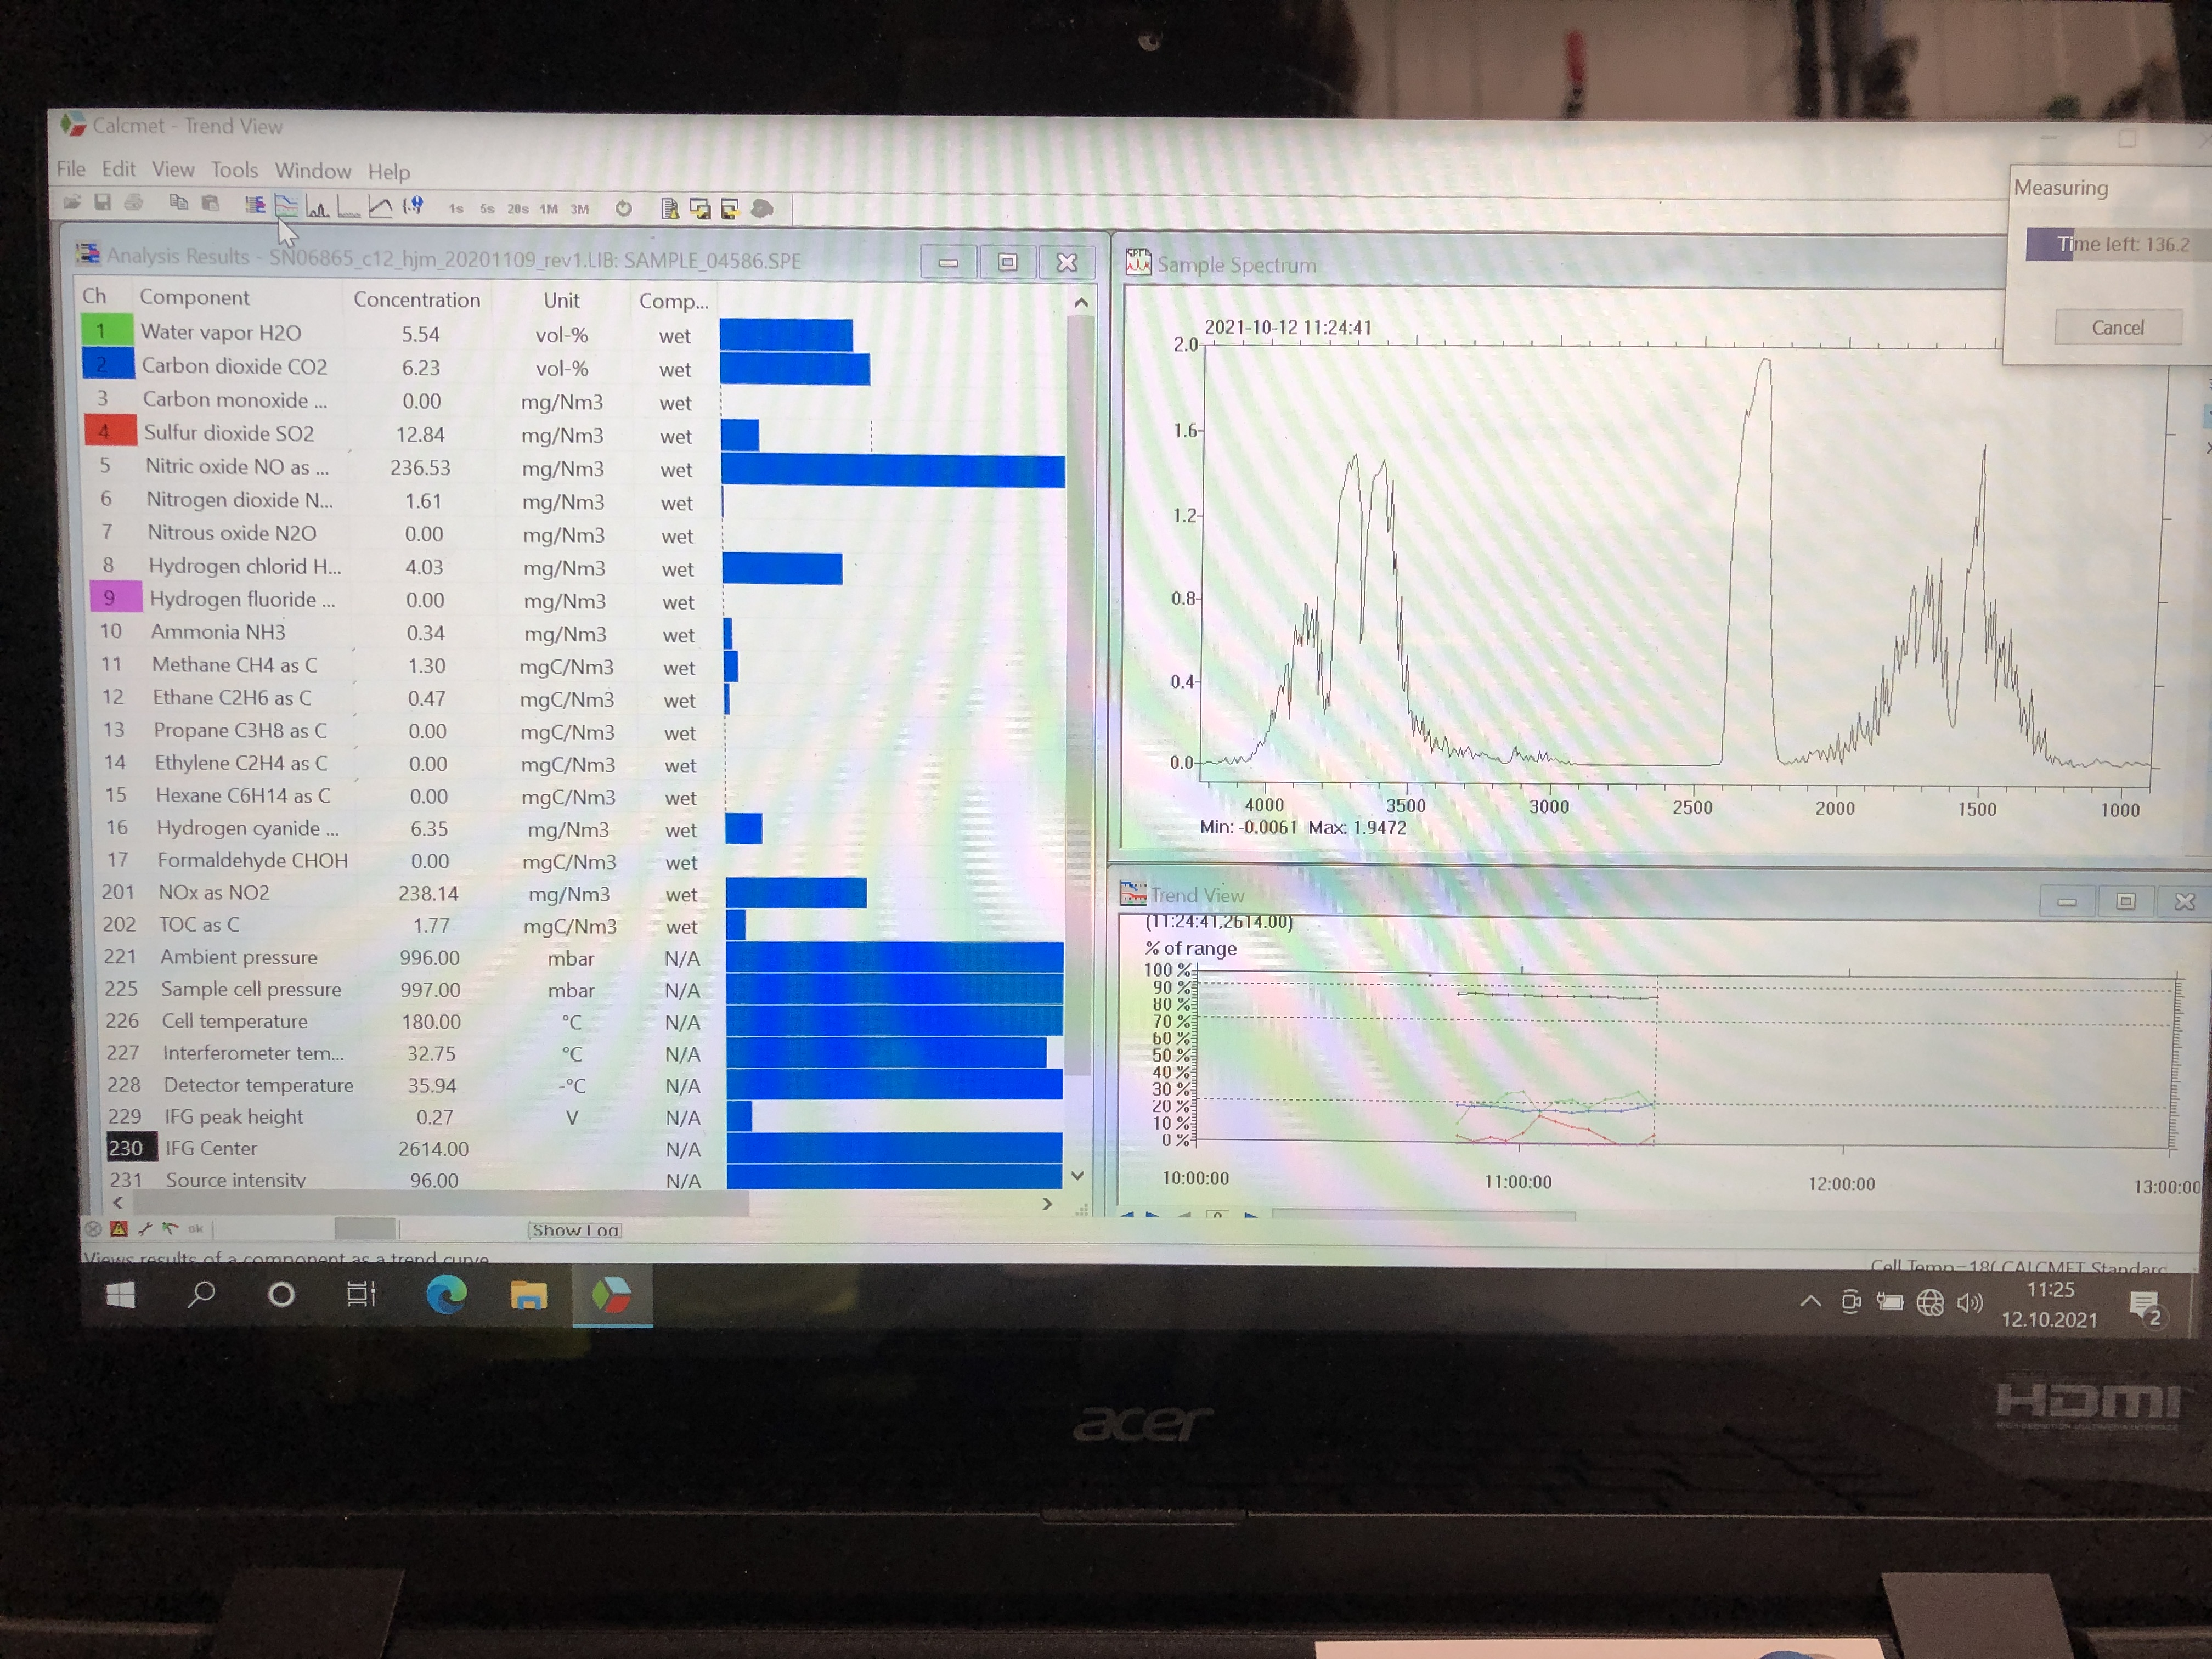
\includegraphics[width=0.6\textwidth]{Bilder/Pyrolysis/FTIRresults.png}
         \caption{}
         \label{appFig:FTIRresults}
     \end{subfigure}
     \hfill
     \caption{(a) FTIR. The tube leading to the FTIR is heated to 180 \textdegree C to prevent condensation of syn-gas. (b) FTIR output results. The results are a screenshot of the FTIR spectra from pyrolysis of Biorest Lindum (BRL).}
    \label{appFig:FTIR}
\end{figure}


\begin{figure}
    \centering
    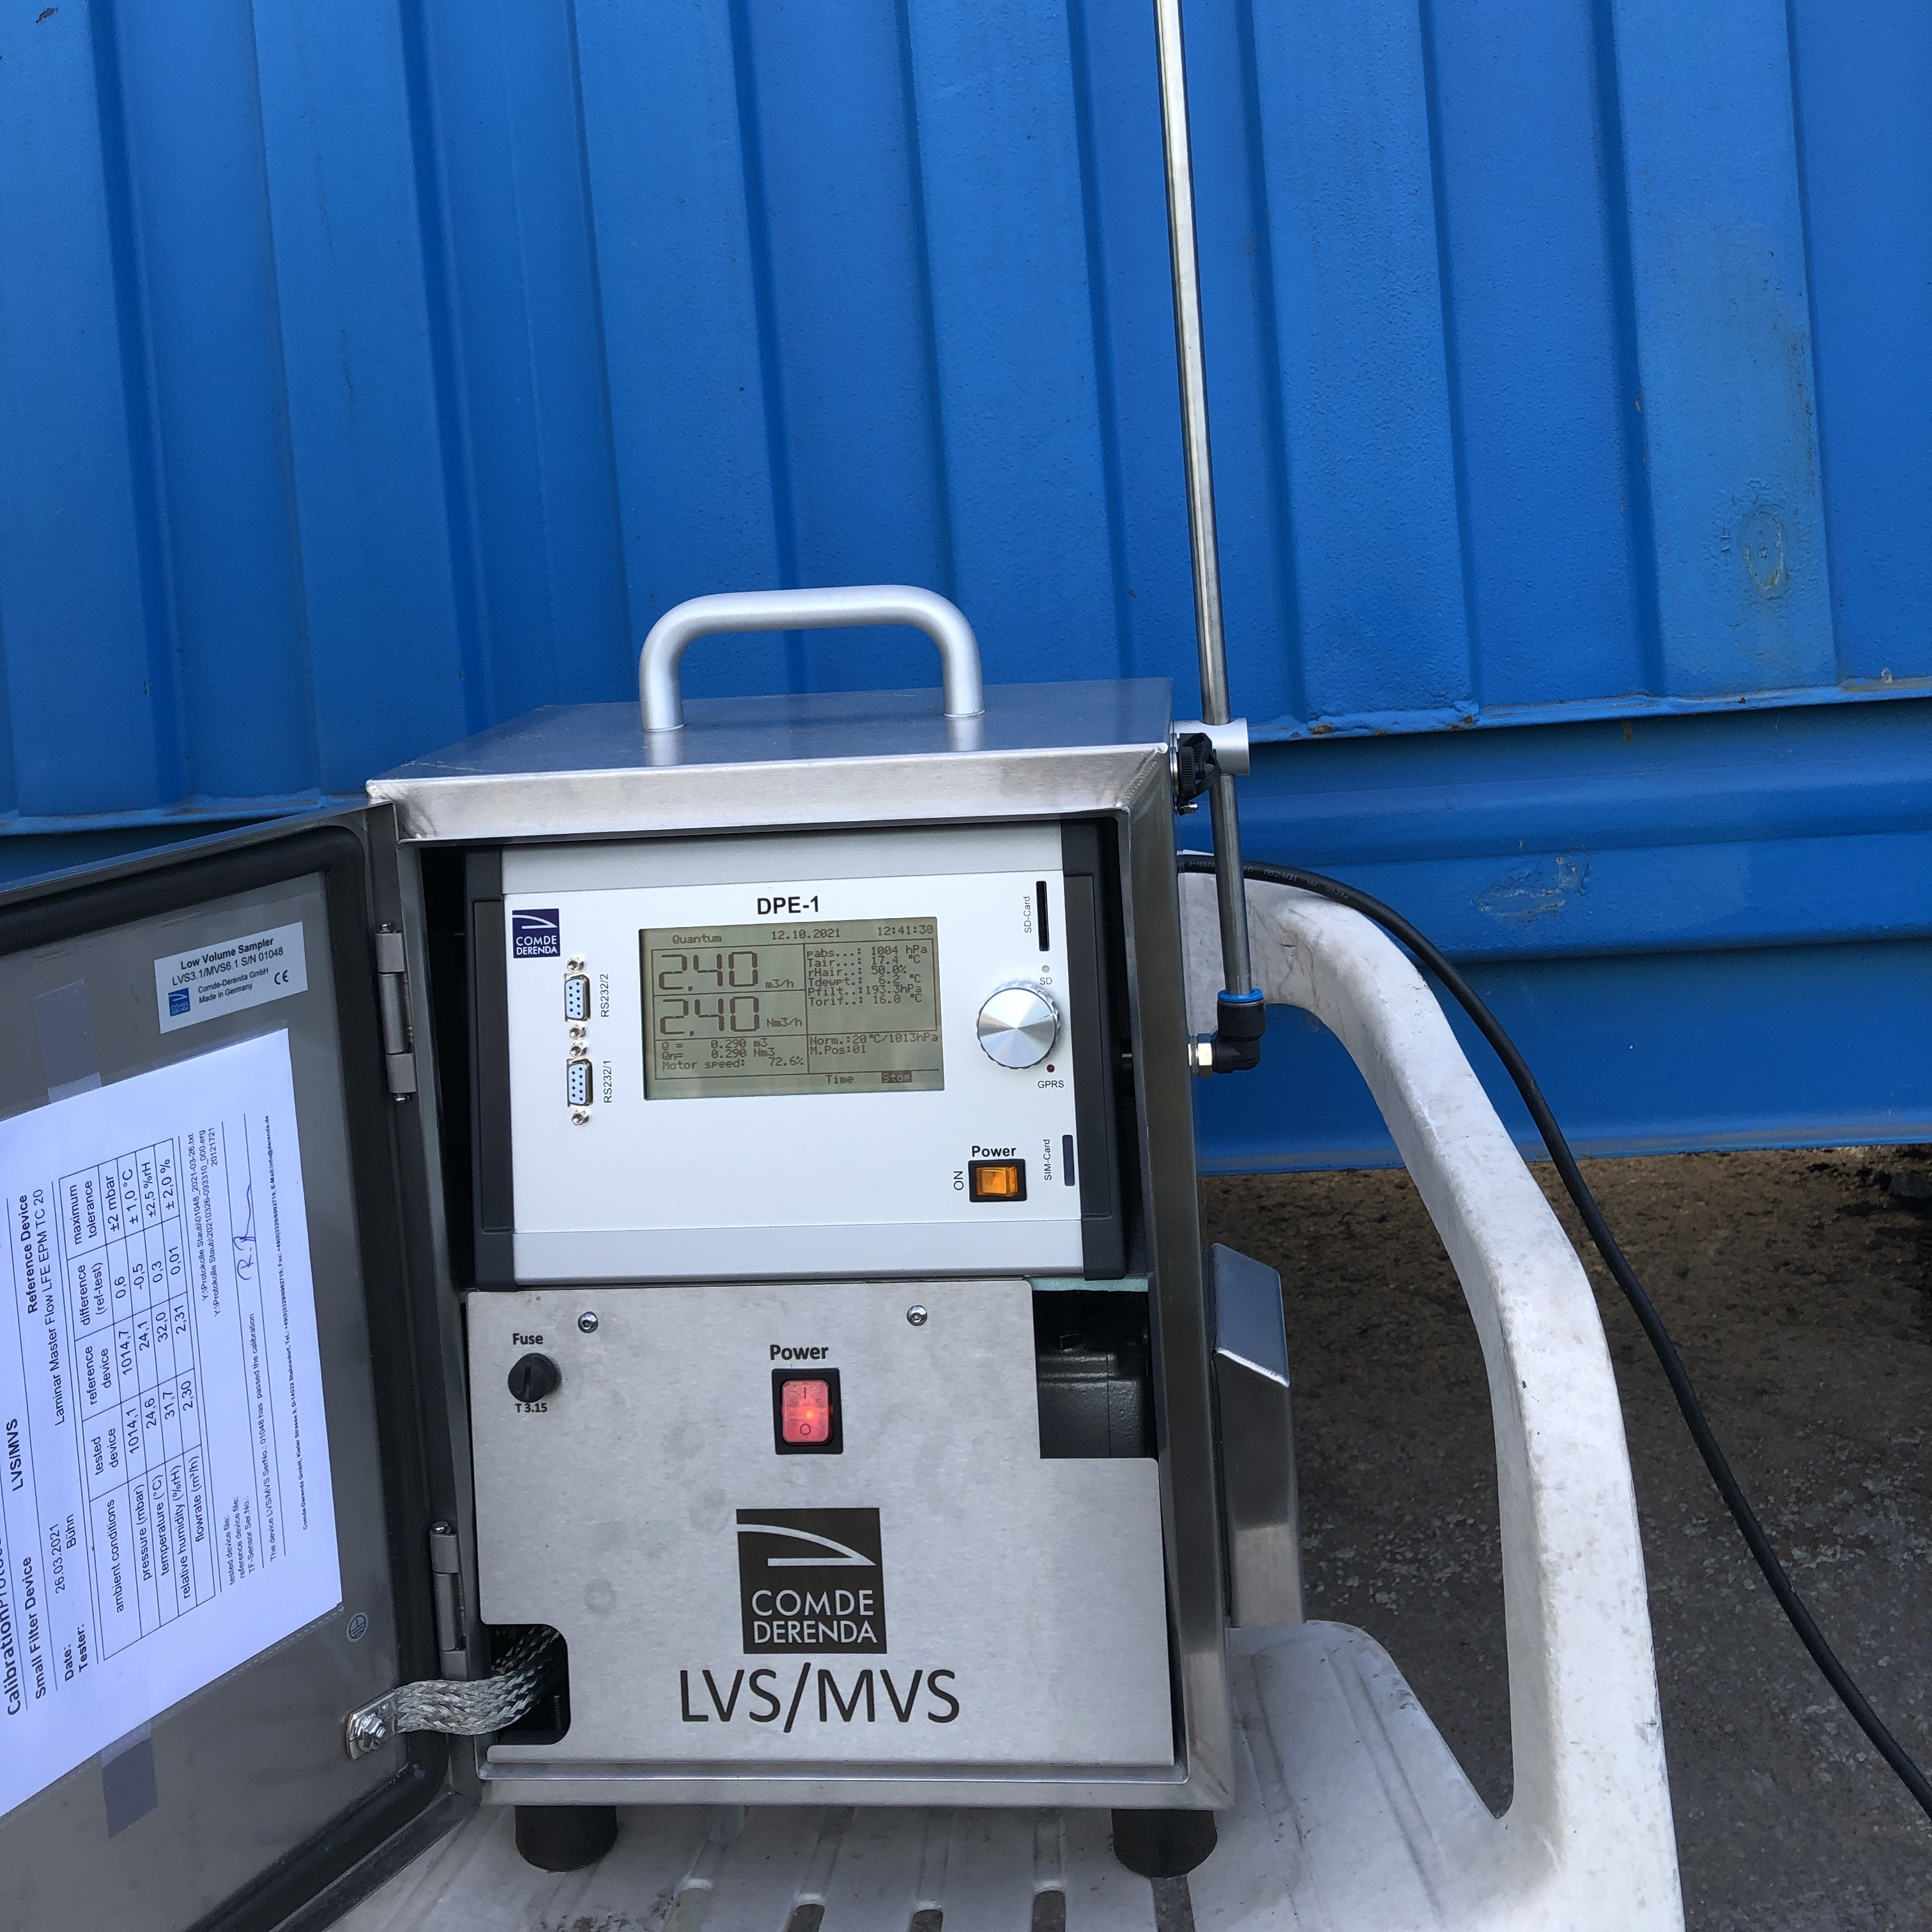
\includegraphics[width=0.85\textwidth]{Bilder/Pyrolysis/ParticlePump.jpg}
    \caption{LVS/MVS vacuum pump draws in air emitted from the ETIA chimney, and the sampler fractionates the airborne fine particles in a sampling inlet. The air containing the desired fine particulate fraction then passes through the filter, where the particles are collected and made available for subsequent gravimetric assessment or analysis. The volumetric flow rate is measured with an orifice plate and electronically adjusted with an accuracy of $\leq$ 2 $\%$. (Copied from comde-derenda.com, bust be rephrased)}
    \label{appFig:ParticlePump}
\end{figure}


\end{document}